% ===========================================================================
%  The body of the complete script -- the chapter order in one place.
%
%  Included by numprog_skript.tex, which builds both the screen and the
%  print version from it, so a chapter added here shows up in both.
%
%  The chapter files sit next to this one in kapitel/, so the paths below
%  are relative to the document -- no \npbase needed.
% ===========================================================================

	\normalsize
	\tableofcontents \label{chap:toc}
	\addtocontents{toc}{\protect\hypertarget{toc}{}}

	\onecolumn
	\normalsize

% ---------------------------------------------------------------------------
% Front matter
% ---------------------------------------------------------------------------
	
	\newpage
	
% =========================================================	
\section{Vorwort}
% =========================================================
	\large
	\vfill
	Dieses Dokument wurde von einem Tutor erstellt. Des Weiteren ist dies kein offizielles Dokument unterstützt oder in Relation mit irgendwelchen Lehrstühlen oder deren Mitarbeitern.
	\\
	Insofern besteht keine Garantie auf \fat{Vollständigkeit oder Korrektheit} der Inhalte.
	\vfill
	
	\noindent Ich habe dieses Skript im Sommersemester 2017 angefangen zu schreiben und seitdem erweitert. Hier könnt ihr Erklärungen, Beispiele sowie Methodiken zu dem gesamten Lernstoff finden. Es soll der \fat{Lernunterstützung und Vorbereitung} auf die Klausur dienen.
	\vfill
	
	\noindent Wie sollte man es nutzen? Ich persönlich empfehle folgendes:
	\begin{enumerate}
		\item Skript durchlesen, Notizen rausschreiben und anhand davon Stoff verstehen.
		\item Übungsaufgaben (wie z.B. in meinem Trainer) durchgehen und erlangtes Wissen überprüfen/vertiefen.
		\item Fragen stellen, falls man etwas nicht verstanden hat.
		\item Die Probeklausuren als finale Vorbereitung durchrechnen.
		\item Richtige Klausur schreiben.
		\item Profit. \Cooley
	\end{enumerate}
	\vfill
	
	\noindent Die aktuellen Dokumente findest du immer auf meiner Webseite:
	\begin{center}
		\href{\npauthorurl}{\npauthorurltext}.
	\end{center} 
	\vfill
	
	\noindent Nun wünsche ich frohes Lernen und viel Erfolg! \Smiley
	\vfill
	
	\noindent Liebe Grüße \\
	Hendrik
	
	\vfill
	\vfill
	\normalsize                    % Vorwort
	
	
	\newpage
% =========================================================	
\section{Legende}
% =========================================================
	
	\vfill
	\bsp{
		\n 
		Beispiele aus Erklärungen und Methoden findet man in diesen Abschnitten.
		\bsp{
			\n
			Diese Box enthält ein Beispiel einer Beispielbox.
		}
	}
	\vfill
	\defi{
		\n 
		Diese Boxen enthalten Texte, die euch ein Thema näher bringen sollen. Verständnis ist das Ziel, weswegen diese Boxen mitunter die wichtigsten sind.
%			Diese Seite erklärt wofür die Boxen alle stehen.
%		}
	}
	\vfill
	\wichtig{
		\n 
		Diese Anmerkungen sollte man nicht überlesen da sie meist wichtige \fat{ABER} und/oder Ausnahmen von Regeln enthalten.
	}
	\vfill
	\methode{
		\n 
		Hier stehen die Schritte einer Methode kurz und knapp beschrieben, um ein gewisses Problem zu lösen. Diese entsprechen in den meisten Fällen dem Schema X, um einen gewissen Aufgabentyp zu lösen.
		\wichtig{
			\n 
			Die Methoden sollten gut gekonnt werden, aber ihr müsst die nicht unbedingt auswendig wissen. Verständnis ist wichtiger als Schema X!
		}
	}
	\vfill
	\vertief{
		\n 
		Vertiefungen, Beweise, Verweise und nennenswerte Fakten stehen in solchen Boxen drin. Der Inhalt könnte nicht prüfungsrelevant sein, aber immer interessant und wissenswert!
	}
	\vfill
	                    % Legende der Infoboxen
		
	\newpage
% =========================================================	
\section{Liste der Notationen}
% =========================================================

	\sbreak
	\begin{center}
		\begin{tabular}{cp{12cm}}
			\toprule
			Notation						&	Beschreibung\\
			\midrule
			$\reals$						&	Die reellen Zahlen. \\%The real numbers including the zero.\\
			$\naturals$						&	Die natürlichen Zahlen, Null enthaltend. \\
			$\complexes$					&	Menge der komplexen Zahlen. \\
			%$\vec{u}$						&	The vector $u$. \\
			$u_i$							&	$i$. Eintrag des Vektors $u$. \\
			$\bigO$							&	Big O Notation für Laufzeitklassen.\\
%			$|x|_n$							&	Die $l_n$ Norm von $x$. \\
			%$f(x)$							&	Eine Funktion, die von $x$ abhängig ist. \\
			$\abs{x}$						&	Absoluter Wert von $x$. \\
			$\norm{x}_2$					&	Normiertes $x$ ($\ell-2$ Norm). \\
			$f'(x)$							&	Die Funktion $f(x)$, einmal abgeleitet. \\
			$f^{(d)}(x)$					&	Die $d$. Ableitung von $f(x)$. \\
			% Matrix Stuff
			$A\trans$						&	Transponierte der Matrix $A$. \\
			$A\inv$							&	Das Inverse der Matrix $A$. \\
			$\diag(A)$						&	Vektor mit den Diagonaleinträgen der Matrix $A$. \\
			$\det(A)$						&	Die Determinante der Matrix $A$. \\
			% operationen
			$\rd(x)$						&	$x$, gerundet. \\
			$y \shouldEq x$					&	$y$ soll gleich $x$ sein. \\
			$y := x$						& 	$y$ ist definiert als $x$. \\
			$y \gg x$						&	$y$ viel größer als $x$. \\
			$y \ll x$						&	$y$ deutlich kleiner als $x$. \\
			$\exp(x)$						&	Andere Schreibweise für $e^x$. \\
			% komplexes zeug
			$\realPart(z)$					&	Realteil einer komplexen Zahl. \\
			$\imaginaryPart(z)$				&	Imaginärteil einer komplexen Zahl. \\
			$\compl{z}$						&	Das komplex konjugierte einer komplexen Zahl $z$. \\
			$\tilde{a}$						&	Eine durch Numerik verfälschte Variable $a$. \\
			\bottomrule
		\end{tabular}
	\end{center}
			
	\newpage
	\begin{center}
		\begin{tabular}{cp{12cm}}
			\toprule
			Notation						&	Beschreibung\\
			\midrule
			% Zahlendarstellungen
			%$\beta$							&	Zahlenbasis \\
			$n$								&	Anzahl Stückstellen oder Anzahl Bits (je nach Kapitel). \\
			% Kondition & Stabilität
			$\fabs$							&	Absoluter Fehler. \\
			$\frel$							&	Relativer Fehler. \\
			$\cond()$						&	Die relative Konditionszahl. \\
			$\maxError$						&	Maschinengenauigkeit (der maximal bei einer Rundung auftretende Fehler). \\
			op								&	Beliebige, exakte Operation. \\
			op$_\text{M}$					&	Eine beliebige, fehlerbehaftete Operation. \\
			% Orthogonal + QR
			$\unitM$						&	Die Einheitsmatrix. \\
			$G_\varphi$						&	Rotationsmatrix bezüglich des Winkels $\varphi$. \\
			% Interpolation
			$c_i$							&	Koeffizient mit Index $i$. \\
			$p(x)$							&	Interpolation (polynoms-) funktion. \\
			$L_j$							&	Lagrange Basis. \\
			$H_i$							&	Kubische Basispolynome. \\
			% Quadratur
			$H$								& 	Insgesamte Größe des zu interpolierenden / integrierenden Bereiches. \\
			$h$								&	Länge eines (oder aller) Bereiche zwischen zwei Stützstellen. \\
			$\QT$							&	Die Trapezregel oder Keplersche Fassregel. \\
			$\QTS$							&	Die Trapezsumme. \\
			$\QS$							&	Simpsonregel. \\
			$\QSS$							&	Simpsonsumme. \\
			% Fourier Transformation
			$\DFT$							&	Diskrete Fourier Transformation. \\
			$\IDFT$							&	Inverse diskrete Fourier Transformation. \\
			$\FFT$							&	Fast Fourier Transformation. \\
			$\BFO$							&	Butterfly Operator. \\
			% Fixpunkte
			$x*$							&	Fixpunkt. \\
			$\Phi(x)$						&	Iterationsvorschrift einer iterativen Methode. \\
			$\delta t$						&	Schrittweite eines Iterationsverfahrens. \\
			% Eigenwerte
			$\lambda(A)$					&	Eigenwerte der Matrix $A$. \\
			$\lambda_{\max}(A)$				&	Der größte Eigenwert der Matrix $A$. \\
			$\mu$							&	Shift einer Power Iteration. \\
			\bottomrule
		\end{tabular}
	\end{center}                   % Notationsverzeichnis

% ---------------------------------------------------------------------------
% Zahlendarstellung
% ---------------------------------------------------------------------------
	
	\newpage
	
% =========================================================	
	\section{Zahlendarstellung} \label{chap:zahlendarstellung}
% =========================================================
	
	\defi{
		\n 
		Zahlendarstellungen sind eine wichtige Grundlage der Numerik. Zunächst betrachten wir die Zahlenbasen, welche für uns relevant sind und wie wir sie übersetzen.
	%}
	%
	%
		\n
		Die wichtigsten Zahlenbasen sind für uns:
		\begin{itemize}
			\item Basis 2, binäre Zahlen genannt,
			\item Basis 10, die Dezimalzahlen und
			\item Basis 16 oder auch Hex-Zahlen.
		\end{itemize}
		Falls eine Darstellung nicht hinreichend gekennzeichnet ist, schreibe ich eine 2 in den Index bei binären Zahlen, bei Hex-Zahlen eine 0x vor die Zahl oder eine 16 in den Index. Falls die Darstellung durch einen Hex-Buchstaben trivialerweise einer Hex-Zahl entspricht, lasse ich eine Kennzeichnung weg.
%	}
%	
		\n 
		In der nächsten Tabelle lasse ich z.B. die Kennzeichnungen weg, da die erste Spalte die Basis der Zahlen angibt.
%	}
% =========================================================
%Zahlenbasen Beispiele (Tabelle)
	\begin{table}[H]
		\centering
			\begin{tabular}{lcccc}
				\toprule
				Basis   & \multicolumn{4}{c}{Beispiele} \\ \midrule
				Binär   & 01100  & 10001 & 11101 & 00011 \\
				Dezimal & 12     & 17    & 29    & 03    \\
				Hex     & 0C     & 11    & 1D    & 03    \\
				\bottomrule
			\end{tabular}%
		\caption{Beispiele für alle Basen.}
		\label{table:basen}
	\end{table}
% =========================================================
	\begin{table}[H]
		\centering
		\begin{tabular}{lccccccccccc}
			\toprule
			Ganzzahl & 1                   & 2                   & 4                   & 8                   & 16                  & 32                  & 64                  & 128                 & 256                 & 512                 & 1024                 \\ \midrule
			Potenzschreibweise & 2$^0$ & 2$^1$ & 2$^2$ & 2$^3$ & 2$^4$ & 2$^5$ & 2$^6$ & 2$^7$ & 2$^8$ & 2$^9$ & $2^{10}$ \\ 
			\bottomrule
		\end{tabular}
		\caption{Die wichtigsten Zweierpotenzen.}
		\label{table:2potenz}	
	\end{table}
% =========================================================
	\begin{table}[H]
		\centering
		\begin{tabular}{lcccccc}
			\toprule
			Hex-Buchstabe & A                   & B                   & C                   & D                   & E                  & F\\ \midrule
			Dezimalwert & 10 & 11 & 12 & 13 & 14 & 15\\ 
			\bottomrule
		\end{tabular}
		\caption{Wdh. Hex Buchstaben.}
		\label{table:hex}
	\end{table}
}

	\newpage
% =========================================================
	\subsection{Dezimal zu Binär}

		Du hast beispielweise die Zahl 12 und möchtest diese binär darstellen.\\
		
		\methode{
			\begin{itemize}
				\item Überlege dir, welche größte Zweierpotenz noch in deine Zahl reinpasst\\
				(Bei $12$ wäre das $8$, also $2^3$)
				\item Subtrahiere deine Zahl durch diese Potenz und schreibe eine \qu{$1$}.
				\item Geh jetzt jeweils durch alle kleineren Zweierpotenzen (bis $2^0$) und subtrahiere deine Zahl durch diese, wenn möglich \\
				(Solang die Subtraktion nicht kleiner null wird)
				\item Immer wenn man die Zahl nicht subtrahieren kann ($< 0$), schreibe eine \qu{$0$}, ansonsten eine \qu{$1$}.
			\end{itemize}
		}
		
		\sbreak	
		\bsp{(von oben)
			\begin{align*}
				12 - 2^{3} &= 4 \imp 1\\
				4 - 2^{2} &= 0 \imp 1\\
				0 - 2^{1} &< 0 \imp 0\\
				0 - 2^{0} &< 0 \imp 0
			\end{align*}
			Somit ergibt sich (von oben nach unten) \qu{$1100_2$}.
		}
				
		\sbreak
		\bsp{ Umwandlung von $37$:
			\begin{align*}
				37 - 2^{5} &= 5 \imp 1\\
				5 - 2^{4} &< 0 \imp 0\\
				5 - 2^{3} &< 0 \imp 0\\
				5 - 2^{2} &= 1 \imp 1\\
				1 - 2^{1} &< 0 \imp 0\\
				1 - 2^{0} &= 0 \imp 1
			\end{align*}
			Das Ergebnis ist \qu{$100101_2$}.
		}

\newpage
% =========================================================	
	\subsection{Binär zu Hex}
		\sbreak
	
		\methode{\n
			Wenn wir eine binäre Zahl in eine hexadezimale Zahl umwandeln wollen, ergeben vier binäre Ziffern jeweils eine Hex-Ziffer der Hex-Zahl.
			Also geht man durch die binäre Zahl von rechts nach links, trennt sie in Viererpakete auf und wandelt dann jedes Paket einzeln um.
		}
		
		\sbreak
		\bsp{ 
			\n
			$101010_2$ zu Hex umwandeln (Das wäre 42 als Dezimalzahl):
			\n
			Auftrennen in Viererpakete: \fat{0010|1010}
			\n 
			Die letzten (rechtesten) vier Ziffern ergeben im Dezimalsystem 10. Dies entspricht in Hex einem \qu{A} (siehe \refTable{table:hex}).
			Das andere Päkchen entspricht einer 2 und in Hex damit einer 2.
			\n 
			Die Hex Zahl ist somit \qu{2A}.
		}
		
		\sbreak
		\bsp{\n 
			Umwandlung von $110110011_2$: 
			\n
			Viererpakete: \fat{0001|1011|0011}
			\n
			Einzelne Umwandlungen: 
			\begin{align*}
				0001_2 &\imp 1& 1011_2 &\imp 11 (= \text{B})& 0011_2 \imp 3
			\end{align*}
			Die Hex Zahl ist somit "1B3"
		}
	
	\newpage
% =========================================================	
	\subsection{Dezimalbrüche zu Binär}
		
		\sbreak
		\methode{\n
			Führe schriftliches Dividieren der Brüche im binären System aus (das geht analog zum dezimalen).
			Das Ergebnis der Division ist auch das Ergebnis der Konvertierung.}
	
		\sbreak
		\bsp{\n
			$\frac{3}{4} = 011_2 : 100_2$
			\begin{table}[H]
				\label{table:dec>binary1}
				\begin{tabular}{llllll}
					0 	& 1 & 1 &   & \multicolumn{2}{l}{: $100_2$ = $0.11_2$} \\ \cline{1-4}
						& 1 & 1 & 0 & &  	\\ 
					- 	& 1 & 0 & 0 & &		\\ \cline{2-5}
						&   & 1 & 0 & 0 &   \\
						& - & 1 & 0 & 0 &   \\ \cline{3-5}
						& & & & 0 &
				\end{tabular}
			\end{table}
			\noindent Das Ergebnis ist also "$0.11_2$".
		}
		
		\sbreak
		\bsp{\n
			$\frac{2}{3} = 010_2 : 011_2$
			\begin{table}[H]
				\label{table:dec>binary2}
				\begin{tabular}{llllll}
					0 & 1 & 0 &   & \multicolumn{2}{l}{: $011_2$ = $0.101_2$} \\ \cline{1-4}
					& 1 & 0 & 0 & \\
					- & 0 & 1 & 1 & \\ \cline{2-4}
					& 0 & 0 & 1 & 0 & (Periodisch)
				\end{tabular}
			\end{table}
			\noindent Hier haben wir den Fall, dass sich die Rechnung ständig wiederholt,
			als nächstes würden wieder eine Null und eine Eins kommen usw.
			\n 
			Das Ergebnis ist also: 
			\begin{align*}
				0.1\overline{01}_2
			\end{align*}
		}
                % Zahlenbasen + Umrechnung
	
% =========================================================	
% =========================================================	
	\newpage
	\subsection{Maschinenzahlen} \label{chap:maschinenzahlen}

		\defi{
			\n 
			Der Computer speichert Zahlen in binärer Form und hat dafür nur begrenzt viel Speicher. Diese Zahlen nennt man \fat{Maschinenzahlen} (kurz M.Zahl).
			\n
			Es stehen allgemein gesprochen $n$ \fat{Bits} für eine Zahl zur Verfügung.
		}
	
	\lbreak
	\subsubsection{2-Komplement-Darstellung}
	
		\defi{\n
			Die 2-Komplement-Darstellung ist eine Möglichkeit, mit Bits (also binär) positive sowie negative Ganzzahlen darzustellen (Ganzzahlen sind solche, die ohne ein Komma auskommen).
			\n
			In dieser Darstellung sind alle Bits normal binär kodiert mit einer Ausnahme. Das vorderste (erste/linkeste) Bit repräsentiert $-2^{n-1}$. 
			\\
			Das bedeutet: Wenn nur das erste Bit eine $1$ ist, stellt die Zahl die kleinst-möglichste Zahl dar. Bei $5$ Bits wäre das z.B. $-2^{5-1} = -2^{4} = -16$ \sbreak \\
			Daraus folgt, dass man mit \textit{n} Bits die Zahlen von $(-2^{n-1})$ bis $(2^{n-1}-1)$ darstellen kann. 
		}
		
		\sbreak
		\bsp{\n
			Mit 5 Bits kann man die Zahlen von -16 [$10000_2$] bis 15 [$01111_2$] darstellen.
		}
		
		\sbreak
		\methode{
			\n
			Wenn man nun umrechnen will, geht man am besten von links nach rechts und addiert alle umgewandelten Ziffern aufeinander (eigentlich analog zu einer binären Zahl).
			\n
			Die Bitstelle im Folgenden wurde von links nach rechts nummeriert.
			Das $n$-te Bit ist also das Bit ganz rechts.
			%
			\begin{table}[H]
				\label{table:komplement-darstellung}
				\centering
				\begin{tabular}{lccccc}
					Stelle des Bits & 1        & 2       & 3       & \dots & $n$   \\ \midrule
					Wert des Bits   & $-2^{n-1}$ & $2^{n-2}$ & $2^{n-3}$ & \dots & $2^0$
				\end{tabular}
				\caption{Darstellung}
			\end{table}
			%
			\noindent \fat{Anmerkung:}
			\\
			Im Grunde sind das normale binäre Zahlen mit Ausnahme des ersten Bits!
		}
			
		\newpage
		\bsp{\n
			Im Folgenden seien 4 Bits verfügbar: \\
			(Zur besseren Übersicht wurde das erste Bit sichtbar getrennt)
			\begin{table}[H]
				\label{table:komplement}
				\centering
				\begin{tabular}{ccc}
					M.Zahl &$\imp$ & Dezimalzahl \\
					0\sep 001 &$\imp$& $1$ \\
					0\sep 101 &$\imp$& $5$ \\
					1\sep 000 &$\imp$& $-8$ \\
					1\sep 001 &$\imp$& $-7$ \\
					1\sep 011 &$\imp$& $-5$
				\end{tabular}
			\end{table}
		}
	
		\sbreak
		\methode{ Eine Zahl zu invertieren (z.B. 5 in -5)
			\n 
			Erst einmal die Zahl in die 2-Komplement Darstellung bringen.
			\begin{itemize}
				\item Bitweise Negation (also nullen zu einsen und andersherum)
				\item Addiere 1 auf die Zahl
			\end{itemize}
			Von Minus nach Plus dann alles rückwärts (statt addieren ist es dann subtrahieren)
		}
	
		\sbreak
		\bsp{\n
			5 in -5 umwandeln:
			\begin{align*}
				5 &\imp 0101 && \text{(Binär schreiben)} \\
				0101 &\imp 1010 && \text{(Bitweise Negation)} \\
				1010 &\imp 1011 && \text{(Addition)}
			\end{align*}
			-7 in 7 umwandeln:
			\begin{align*}
			-7 &\imp 1001 && \text{(Binär schreiben)} \\
			1001 &\imp 1000 && \text{(Subtraktion)} \\
			1000 &\imp 0111 && \text{(Bitweise Negation)}
			\end{align*}
		}

% =========================================================	
% =========================================================	
	\newpage
	\subsubsection{Gleitkommazahlen} \label{chap:gleitkommazahlen}
	
		\defi{
			\n 
			Nun möchten wir aber auch reelle Zahlen, oder Approximationen solcher, darstellen können. Das nennen wir die Gleitkommazahlen (im englischen "floating point numbers"). 
			\n 
			Für diese benötigen wir das Verständnis von binären Kommazahlen, also hier eine kurze Wiederholung:
			\begin{table}[H]
				\label{table:binary_kommazahlen}
				\centering
				\begin{tabular}{lccccccc}
					\toprule
					Binär & $1.0_2$ & $0.1_2$ & $0.01_2$ & $0.001_2$ & $0.0001_2$ & $0.00001_2$ &\dots \\
					Dezimalwert & 1 & \nicefrac{1}{2}     & \nicefrac{1}{4}  & \nicefrac{1}{8}   & \nicefrac{1}{16}  & \nicefrac{1}{32} & \dots \\ \bottomrule
				\end{tabular}
				\caption{Wdh. Binäre Kommazahlen}
			\end{table}
		}
		
		\sbreak
		\bsp{
			\begin{table}[H]
				\centering
				\begin{tabular}{ccc}
					\toprule
					Binäre Zahl &$\imp$& Dezimalzahl \\ \midrule
					$1.11_2$ &$\imp$& $1.75$ \\
					$111.001_2$ &$\imp$& $7.125$ \\
					$0.01_2 + 0.01_2 = 0.1_2$ &$\imp$& $\nicefrac{1}{4} + \nicefrac{1}{4} = \nicefrac{1}{2}$ \\
					\bottomrule
				\end{tabular}%
				\caption{Binäre Kommazahlen und deren dezimales Äquivalent.}
				\label{table:bsp_binary_kommazahlen}
			\end{table}
		}

% =========================================================	
	
		\newpage
		\defi{ \n 
			Gleitkommazahlen bestehen (in den meisten Darstellungen) aus \fat{Vorzeichen, Exponent und Mantisse.}
			\begin{align}
				\text{Wert der Gleitkommazahl = } (-1)^{\text{Vorzeichen}} \cdot 2^{\text{Exponent}} \cdot \text{Mantisse}_2
			\end{align}
			Abgekürzt schreibt man das häufig auch:
			\begin{align*}
				\text{G} = (-1)^{\text{V}} \cdot 2^{\text{E}} \cdot \text{M}
			\end{align*}
			Man kann sich die Zahl so vorstellen, dass der Exponent lediglich eine Kommaverschiebung ist. Zum Beispiel gilt 
			\begin{align*} 
				(1.0)_2 \cdot 2^0 = (0.01)_2 \cdot 2^2 = (1000)_2 \cdot 2^{-3} 
			\end{align*}
			In dezimal wäre das:
			\begin{align*} 
				1 \cdot 1 = \frac{1}{4} \cdot 4 = 8 \cdot \frac{1}{8} 
			\end{align*}
		}
		
		\sbreak
		\wichtig{
			\n
			Ohne eine Normierung ist die Darstellung nicht eindeutig, was bedeutet, dass es zur einer (dezimal) Zahl mehrere Möglichkeiten gibt, diese korrekt darzustellen (siehe oben). Also wenn zwei Zahlen (ohne Normierung) verglichen werden, muss nicht zwangsläufig diejenige Gleitkommazahl größer sein, die den größeren Exponenten hat!
		}
		
		%Eine Mantisse ist genau dann normiert, wenn diese eine
		%führende Eins hat und sofort ein Komma folgt.
		
		\sbreak
		\defi{ Normierung 
			\n
			Bei einer normierten Mantisse wird der Exponent genau so gewählt, dass die Mantisse eine von Null verschiedene Stelle vor dem Komma hat (also dass die Mantisse die Form 1, \dots hat). So löst sich auch der letzte \red{Wichtig}-Block. Das machen wir aus dem Grund, da nun jede Zahl eine eindeutige Darstellung hat. Also ist die Mantisse genau dann normiert, wenn diese eine führende Eins hat und sofort ein Komma folgt.
			\n
			Damit bezeichnet die normierte Mantisse unsere Nachkommastellen (plus die Eins vor dem Komma).
		}
		
		\sbreak
		\bsp{
			\n
			Eine dezimale $16$ würde man von $(0.1)_2 \cdot 2^5$ zu $(1.0)_2 \cdot 2^4$ normieren.
		}
	
% =========================================================	
	%\lbreak
	\newpage
	\subsubsection{IEEE-Standard} \label{chap:ieee}
	
		\defi{
			\n 
			Der sogenannte IEEE Standard ist eine Darstellungsmöglichkeit, die in vielen Bereichen verwendet wird. Ihr stehen 32 Bits zur Verfügung, die folgende Verteilungen besitzen:
			\begin{itemize}
				\item 1 Bit für das Vorzeichen: \\
				Null für positiv, Eins für negativ
				\item 8 Bits für den Exponenten: \\
				Der Exponent soll aber auch negative Werte annehmen können, eine Erklärung wie das gemacht wird folgt noch.
				\item 23 Bits für die Mantisse (Nachkommastellen): \\
				Von einer Normalisierung mit führender Eins wird ausgegangen.\\
				Diese Eins muss \fat{nicht} abgespeichert werden, wodurch man sich ein Bit spart.
				\item Genügen 23 Bits nicht für die Darstellung, muss gerundet werden.
			\end{itemize}
			Der Exponent entspricht einer normalen binären Zahl, aber da man negative Werte darstellen möchte, zieht man eine Konstante ab. So shiftet man den darstellbaren Bereich für den Exponenten von 0 bis $(2^n-1)$ auf $(-2^{n-1} +1)$ bis $(2^{n-1})$. Die Konstante entspricht also $(2^{n-1} - 1)$. Im Beispiel der 8 Bits des Exponenten würde also die binäre Zahl um 127 verringert werden, damit man den eigentlichen Exponenten hat.
			%Die Binärzahl entspricht dem (Dezimal-)Exponenten + 127. Andersherum: Der (Dezimalwert minus 127) entspricht dem Exponenten in der IEEE Darstellung.
			%Warum +127 beim Exponenten? \\
			%Damit wir (ähnlich der 2-Komplement Darstellung) Exponenten von -127 bis 128 darstellen können anstelle von 0 bis 256.
		}
	
		\sbreak
		\bsp{ 
			\begin{table}[H]
				\centering
				\begin{tabular}{ccc}
					\toprule
					Abgespeicherten Bits   & & Wert \\ \midrule
					01111101 & $\imp$ & $-2$ \\
					00000001 & $\imp$ & $-126$ \\
					11111110 & $\imp$ & $127$ \\
					10000000 & $\imp$ & $1$ \\
					\bottomrule
				\end{tabular}%
				\caption{Beispiele der IEEE Exponenten und ihre tatsächlichen Werte (wegen dem konstanten Abzug von 127).}
				\label{table:ieeeExponent}
			\end{table}
%				(Da der Dezimal wert 125 ist, minus 127 ist gleich -2)
%				(0, Infinity, NaN, \dots)
		}
	
		\wichtig{ \n
			$00000000_2$ und $11111111_2$ des Exponenten sind allerdings speziell reserviert (0, Infinity, NaN, \dots).
		}
	
		\sbreak
		\methode{ Dezimalzahl in IEEE umwandeln:
			\begin{itemize}
				\item Dezimalzahl in binäre Zahl umwandeln,
				\item Exponent so bestimmen, dass die restliche Zahl (Mantisse) normiert ist,
				\item Vorzeichen direkt umwandeln (Eins für negative, Null für positive Zahl),
				\item Exponent $+127$ nehmen und dann in binär umwandeln,
				\item Mantisse einfach hinschreiben (die Eins vor dem Komma weglassen!) und wenn nötig runden.
			\end{itemize}
		}
	
		\sbreak
		\bsp{
			\begin{table}[H]
				\centering
				\begin{tabular}{cccc}
					\toprule
					Dezimal & Binär 		& Gleitkommadarstellung 	& IEEE (V | E | M)\\ \midrule
					$32.00$ & $100000_2$ 	& $2^5 \cdot 1.0_2$ 		& $0|10000100|00000000000000000000000$ \\ \greyMidRule
					$13.75$ & $1101.11_2$ 	& $2^3 \cdot 1.10111_2$ 	& $0|10000010|10111000000000000000000$\\ \greyMidRule
					$-0.125$ & $-0.001_2$ 		& $-1 \cdot 2^{-3} \cdot 1.0_2$ & $1|01111100|00000000000000000000000$\\
					\bottomrule
				\end{tabular}%
				\caption{Beispiele von Dezimalzahlen und ihre dazugehörige normierte Gleitkommadarstellung und wie die 32 Bits in IEEE aussehen würden.}
				\label{table:bsp_gleitkommazahlen}
			\end{table}
		}
	
%			Gute Umformungsregeln für das IEEE-Format kann man hier finden:
%			Einen Umrechnungsrechner kann man hier finden:
%			Eine bildliche Veranschaulichung inklusive Erklärungstext für Umwandlung in das IEEE-Format ist unter:
%		}

	\newpage
% =========================================================	
	\subsubsection{Rundung} \label{chap:rundung}
	
	\defi{
		\n
		$\rd(x)$ ist die Zahl, die herauskommt, wenn man $x$ rundet.
		\n
		Aber \fat{wie} rundet man denn überhaupt bei Gleitkommazahlen? \\
		Im Folgenden sei eine Zahl bis zu dem Zeichen "|" korrekt darstellbar (sprich alle Zahlen dahinter müssen gerundet werden).
	}
	
%	}
	
	\sbreak
	\methode{ \n 
		Es gibt vier Fälle für das Runden. Sei $y$ jeweils beliebig:
		\begin{align*}
			&y \sep 0x \quad \text{ mit $x$ "beliebig"} &&\imp \text{Abrunden} \\%\label{eq:round} \\
			&y \sep 1x \quad \text{ mit $x$ "nicht nur Nullen"} &&\imp \text{Aufrunden}\\
			&y1 \sep 1x \quad \text{ mit $x$ "nur Nullen"} &&\imp \text{Aufrunden}\\
			&y0 \sep 1x \quad \text{ mit $x$ "nur Nullen"} &&\imp \text{Abrunden}
		\end{align*}
	}

	\sbreak
	\wichtig{
		\n 
		Die letzten beiden Regeln des vorangegangenen Blocks werden häufig auch die "uneindeutigen Fälle" genannt, je nach Notation und Darstellung können die Rundungsregeln dafür anders definiert sein (oben sind sie so definiert, dass sie immer zur geraden Mantisse gerundet wird). Schaut also hierbei, was in der Klausur angegeben ist!
	}
	
	\sbreak
	\bsp{
		\begin{table}[H]
			\centering
			\begin{tabular}{ccc}
				\toprule
				Originalzahl & Gerundet & Aktion\\ \midrule
				$1.0\sep 1010_2$ & $1.1_2$ & Aufgerundet \\
				$1.0\sep 0111_2$ & $1.0_2$ & Abgerundet \\
				$1.1\sep 1000_2$ & $10_2$ & Aufgerundet \\
				$1.0\sep 1000_2$ & $1.0_2$ & Abgerundet \\
				\bottomrule
			\end{tabular}%
			\label{table:bsp_rundung}
		\end{table}
%			&1.0\sep 101_2 &&\imp 1.1_2 &&\text{(Aufgerundet)} \\
%			&1.0\sep 0111_2 &&\imp 1.0_2 &&\text{(Abgerundet)} \\
%			&1.1\sep 1000_2 &&\imp 10_2 &&\text{(Aufgerundet)} \\
%			&1.0\sep 1000_2 &&\imp 1.0_2 &&\text{(Abgerundet)}
	}
		
	\newpage
	\defi{
		\n 
		Durch Rundungen entstehen jedes Mal Fehler. Wir unterscheiden zwischen folgenden Fehlertermen.
		\n 
		Absoluter Fehler: 
		\begin{align} 
			 \fabs := \abs{x - \rd(x)} 
		\end{align}
		Relativer Fehler:
		\begin{align} 
			\frel := \abs{\frac{\fabs}{x}} 
		\end{align}
	}

	\sbreak
	\bsp{
		\n 
		Sei eine Zahl $x$ bis zu dem Zeichen "|" exakt darstellbar. Mit $x = 10.0|11_2$ wird aufgerundet (siehe oben). Also ist $\rd(x) = 10.1_2$.
		\n 
		Der absolute Fehler dieser Rundung beträgt:
		\begin{align*} 
			\fabs(x) &= \abs{x - \rd(x)} \\
				&= \abs{10.011_2 - 10.1_2} \\
				&= 0.001_2 \\
				&= \frac{1}{8}
		\end{align*}
		Den relative Fehler können wir dann wie folgt bestimmen:
		\begin{align*} 
			\frel(x) &= \abs{\frac{\fabs}{x}} \\
				&= \abs{\frac{\nicefrac{1}{8}}{10.011_2}} \\
				&= \abs{\frac{\nicefrac{1}{8}}{2.375}} \\
				&= \abs{\frac{1}{8} \cdot \frac{8}{19}} \\
				&= \frac{1}{19}
		\end{align*}
	}
	
% =========================================================	
	\newpage
	\subsubsection{Maschinengenauigkeit} \label{chap:maschinengenauigkeit}
	
	\defi{ \n 
		Die Maschinengenauigkeit beschreibt die größte positive Zahl $x$, sodass $\rd(x+1) = 1$ gilt. \n
		Wird berechnet durch: 
		\begin{align} 
			\epsilon = \frac{1}{2} \cdot \beta^{1-t} 
		\end{align}
		\begin{itemize}
			\item $\epsilon$ = Maschinengenauigkeit
			\item $\beta$ = Zahlenbasis (bei uns immer 2)
			\item $t$ = Mantissenlänge \\
			(bei IEEE ist dies 24, weil 23 Bits plus die nicht abgespeicherte Eins)
		\end{itemize}
		Damit beschreibt die Maschinengenauigkeit das Maß der Rundungsfehler, sie gibt also den maximalen relativen Rundungsfehler (bei der Darstellung von Zahlen) an. Mit anderen Worten: Egal wie präzise und genau ein Algorithmus ist, in aller Regel kann er nicht genauer als die Maschinengenauigkeit sein (deswegen der Name \Winkey).
	}

	\sbreak
	\bsp{
		\n 
		Mit IEEE (siehe \refChapter{chap:ieee}) wäre die Maschinengenauigkeit also:
		\begin{align*}
			\epsilon_{\text{IEEE}} &= \frac{1}{2} \cdot \beta^{1-t} \\
				&= \frac{1}{2} \cdot 2^{1-24} \\
				%&= \frac{1}{2} \cdot 2^{-23} \\
				&= 2^{-24}
		\end{align*}
		$1 + 2^{-24}$ im IEEE-Format ergibt gerundet noch genau Eins.
	}
	
%==========================================================	
	\newpage
	\subsubsection{Absorption} \label{chap:absorption}
	
	\defi{ \n
		Ein Problem der Gleitkommaarithmetik ist die sogenannte \fat{Absorption}.
		\n
		Diese findet statt, wenn bei der Addition zwei sehr unterschiedlich großer Zahlen Information verloren geht aka gerundet werden muss.
	}
	
	\sbreak
	\bsp{ \n
		Man möchte $0.75$ auf $7$ aufaddieren, hat aber nur 3 Bits für die Mantisse zur Verfügung.\\
		Zu rechnen: 
		\begin{align*}
			111_2 + 0.11_2 = 111.11_2
		\end{align*}
		$111.11_2$ ist nicht mit 3 Bits darstellbar und führt damit zu einem Rundungsfehler!
		\n 
		In diesem Beispiel würde das Ergebnis aufgerundet werden und damit $1000_2$ ergeben. Das wäre in dezimal eine $8$. Mit exakter Arithmetik wäre es aber $7.75$, wir haben einen absoluten Fehler von $0.25$. Die $7$ hat die $0.75$ absorbiert, nennt man dann so.
	}
	
	\sbreak
	\wichtig{ \n 
		Aus Absorption können wir folgendes herleiten: Bei Gleitkommazahlen geht die Eigenschaft des Assoziativgesetzes verloren!
	}
	
	\newpage
	\subsubsection{Auslöschung} \label{chap:auslöschung}
	
	\defi{\n	
		Unter \fat{Auslöschung} versteht man den Verlust an Genauigkeit, wenn man zwei fast gleich große Gleitkommazahlen subtrahiert. Denn wenn man dies rechnet, rundet sich das Ergebnis zu einer Null, was verheerende Folgen haben kann. In aller Regel ist Auslöschung schlimmer als Absorption.}
	
	\sbreak
	\bsp{ \n
		Sei
		\begin{align*}
			a = 2.3546; \quad b = 2.3510
		\end{align*}
		Seien Zahlen im dezimalen nur auf 3 Ziffern genau darstellbar und der Rest jeweils normal nach der nächsten Ziffer gerundet.
		\n
		Wenn wir jetzt auf die korrekten Ziffern kürzen:
		\begin{align*}
			2.35 - 2.35 = 0
		\end{align*}
		Dabei wäre es analytisch: 
		\begin{align*}
			2.3546 - 2.3510 = 0.0036 \quad \Longrightarrow \text{Keine einzige korrekte Ziffer!}
		\end{align*}
		}
	
	\sbreak
	\vertief{
		\n 
		Warum das so verheerend ist, kann man sich gut aus dem Beispiel erschließen. Denn gehen wir mal davon aus, dass wir nach der Operation aus dem Beispiel nur noch Multiplikationen ausführen müssen. Dann würde im verfälschten Fall immer Null das Ergebnis sein, exakt aber etwas völlig anderes!
		\n 
		Beispielsweise nach obiger Rechnung wird das Ergebnis (aus welchen Grund auch immer) mit $1000$ multipliziert. Dann würde als verfälschte Lösung $0$ rauskommen, exakt wäre aber eigentlich $3.6$.
	}
            % Zweierkomplement + Gleitkommazahlen

% ---------------------------------------------------------------------------
% Fehleranalyse
% ---------------------------------------------------------------------------
	
	\newpage
% =========================================================	
	\section{Kondition} \label{chap:kondition}
% =========================================================
	
	\defi{
		\n
		Die Kondition beschreibt das Fehlerverhältnis zwischen Eingabe und Ausgabe. Man spricht von "guter" oder "schlechter" Kondition, es ist also ein qualitativer Begriff.
		\n 
		Die berechenbare Zahl, die Konditionszahl, entspricht dem ungünstigsten Faktor der Störung. Eine hohe Kondition bedeutet, dass ein Fehler in der Eingabe zu einem noch viel höherem Fehler in der Ausgabe führt.
		Die relative Konditionszahl $\cond(f, x)$ wird folgendermaßen in Abhängigkeit von einer Funktion $f(x)$ berechnet:
		\begin{align} 
	 		\cond(f,x) = \abs{\frac{x \cdot f'(x)}{f(x)}}
	 	\end{align}
		Man unterscheidet generell folgende Fälle:
		\begin{itemize}
			\item $\cond(f, x) \le 1$\\
				Da die Kondition den Fehlerfaktor beschreibt, bedeutet eine Eins, dass es maximal zu keiner Zunahme des relativen Fehlers kommt. Es ist "gut konditioniert".
			\item $\cond(f, x) \gg 1$\\
				Der Fehlerfaktor ist deutlich größer eins und nimmt somit zu. Die Funktion ist "schlecht konditioniert".
				%In diesem speziellen Fall ist die Funktion sehr gut konditioniert, da der Fehler sogar abnimmt.
		\end{itemize}
		%
		\begin{figure}[H]
			\centering
			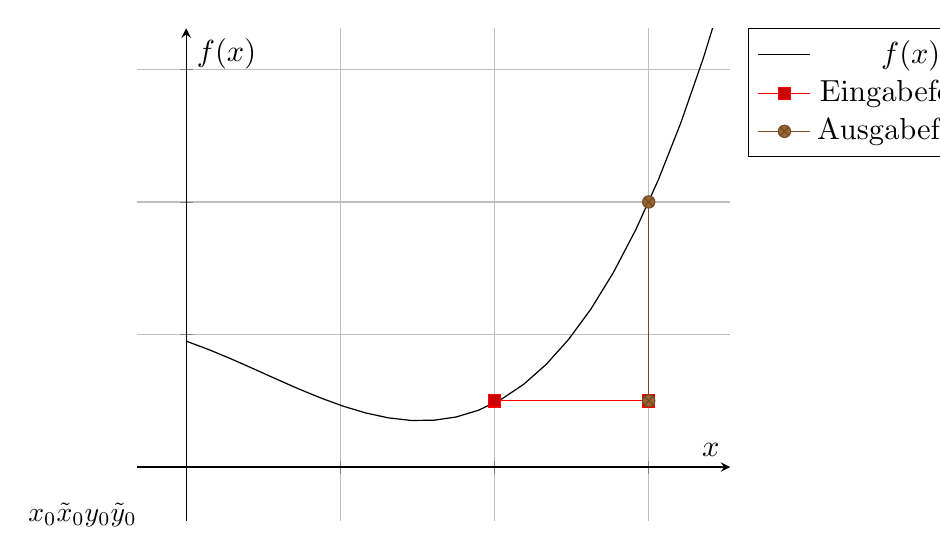
\begin{tikzpicture}[scale=1.1]
				\begin{axis}[
					axis lines=middle,
					xlabel=$x$,
					ylabel=$f(x)$,
					enlargelimits,
					legend pos=outer north east,
					%cycle list name=black white,
					grid=major,
					ymax=6,
					ymin=-0.2,
					xticklabels={,,},
				 	yticklabels={,,},
					]
					\addplot[domain=0:3.5] {1.9 - 0.8*x - 0.5*x^2 + (1/3)*x^3} node[left]{};
					\addplot coordinates {
						( 2, 1 )
						( 3, 1 )
					};
					\addplot coordinates {
						( 3.0, 1 )
						( 3.0, 4 )
					};
					\tikzPointDL{$x_0$}{2,0}
					\tikzPointDL{$\tilde{x}_0$}{3,0}
					\tikzPointUL{$y_0$}{0,1}
					\tikzPointUL{$\tilde{y}_0$}{0,4}
					\legend{$f(x)$, Eingabefehler, Ausgabefehler}
				\end{axis}
			\end{tikzpicture}
			\caption{Plot einer Funktion $f(x)$ und ein Beispiel, wie die Kondition funktioniert. Die exakte Eingabe sei $x_0 = 2$ und wurde durch vorherige Operationen verfälscht ($\tilde{x}_0$). Die Differenz $\abs{\tilde{x}_0 - x_0}$ nennt man den \fat{Eingabefehler}. Dieser führt zu einer Veränderung der Ausgabe, also des $y$-Wertes. Der sogenannte \fat{Ausgabefehler} beschreibt dann die Differenz zwischen der verfälschten Ausgabe $\tilde{y}_0$ und der exakten $y_0$.}
		\end{figure}
	}

	\sbreak
	\bsp{
		\begin{itemize}
			\item $f(x) = x$
				\begin{align*} 
					\cond(f, x) = \abs{\frac{x \cdot 1}{x}} = 1  &&\Longrightarrow \text{gut konditioniert}
				\end{align*}
				Logisch, weil wir die Eingabe ja gerade wieder ausgeben. Wie soll sich da der Fehler der Eingabe überhaupt verändern?
				\sbreak
			\item $g(x) = x^2$
				\begin{align*} 
	 				\cond(g, x) = \abs{\frac{x \cdot 2x}{x^2}} = \frac{2x^2}{x^2} = 2 && \Longrightarrow \text{immer noch gut konditioniert}
	 			\end{align*} 
	 			\sbreak
			\item $h(x) = e^x$
				\begin{align*} 
	 				\cond(h, x) = \abs{\frac{x \cdot e^x}{e^x}} = \abs{x}
	 			\end{align*}
				Fallunterscheidung:
				\begin{align*}
					&\abs{x} \le 1 && \Longrightarrow \text{gut konditioniert} \\
					&\abs{x} \gg 1 && \Longrightarrow \text{schlecht konditioniert}
				\end{align*}
				\sbreak
			\item $i(x) = 1$
				\begin{align*} 
	 				\cond(i, x) = \abs{\frac{x \cdot 0}{1}} = 0 && \Longrightarrow \text{Fehler sind irrelevant}
	 			\end{align*}
				Es ist "perfekt konditioniert". Logisch, da die Ausgabe nicht abhängig von der Eingabe ist. Wie soll die Ausgabe also von einem Eingabefehler überhaupt beeinflusst werden?
		\end{itemize}
	}
                  % Kondition
	
% =========================================================
	\newpage
	\section{Stabilität}	
	
	
	\defi{
		\n
		Ein Verfahren heißt "stabil", wenn Rundungen von Zwischenergebnissen keine große Abweichung der Endergebnisse zur Folge hat; ansonsten spricht man von einem "instabilen" Algorithmus. \n	
		Bei der Stabilitäts Untersuchung geht es darum, die Fehlerverstärkung innerhalb eines Berechnungsverfahrens zu analysieren. Instabil kann nur eine Verkettung von Operationen sein, einzelne sind immer stabil!
		\n	
		Weil viele damit Schwierigkeiten haben sind hier nochmal knapp die Erläuterung von Stabilität \& Kondition:
		\begin{itemize}
			\item \fat{Kondition}
			\begin{itemize}
				\item Ist eine Eigenschaft eines Problems.
				\item Sagt aus, wie groß sich ein Eingabefehler auf die Ausgabe auswirkt.
				\item Quasi $f(\rd(x)) - f(x)$.
			\end{itemize} 
			\item \fat{Stabilität}
			\begin{itemize}
				\item Ist eine Eigenschaft eines Algorithmus.
				\item Sagt aus, ob sich der relative Fehler durch Rundungen stark verschlechtert oder nicht.
				\item Quasi $\rd(f(x)) - f(x)$.
			\end{itemize}			
		\end{itemize}
		Um die Stabilität zu untersuchen verwenden wir Epsilontik.
	}

% =========================================================	
	\sbreak
	
	\defi{ \fat{Epsilontik}
		\n	
		Wir haben ja schon gelernt, dass das Ergebnis einer (auch sehr einfachen) Operation, die ich jetzt allgemein "op" nenne, nicht mehr als Maschinenzahl exakt darstellbar sein kann und dadurch gerundet werden muss (siehe \refChapters{chap:absorption}{chap:auslöschung}). \n	
		Außerdem haben wir gelernt, dass bei Rundungen immer ein relativer Fehler entsteht. Für diesen Fehler $\epsilon$ gilt immer $\abs{\epsilon} \le \maxError$. Dieses $\maxError$ ist hierbei die maximale Fehlergrenze und entspricht der Maschinengenauigkeit der Darstellung (siehe \refChapter{chap:maschinengenauigkeit}).
		\begin{align} 
 			\frel = \abs{\frac{\rd(x) - x}{x}} \le \maxError. 
 		\end{align}
		 Das heißt aber auch, dass es immer ein $\epsilon \in \reals$ geben muss, damit: $\rd(x) = (1 + \epsilon) \cdot x;$ mit $-\maxError \le \epsilon \le \maxError$ \n	
		Diese Eigenschaft verwenden wir bei der Epsilontik. Wir untersuchen den relativen Endergebnisfehler:
		\begin{align} 
 			\abs{\frac{\rd(f)(x) - f(x)}{f(x)}} 
 		\end{align}
		Dabei gelten noch folgende Regeln: \\
		Mit "op" als exakte Operation erzeugt jede Operation "op$_\text{M}$" einen Fehler $\epsilon_i \le \maxError$:
		\begin{align}
			(a \text{ op}_\text{M } b) = \rdM(a \text{ op } b) = (a \text{ op } b) \cdot (1 + \epsilon_i) &&\text{ mit } \abs{\epsilon_i} \le \maxError
		\end{align}
	 	Außerdem lassen wir Fehler höherer Ordnung weg, da wir davon ausgehen, dass unsere Fehler $\epsilon_i$ sehr klein sind und somit $\epsilon_i \cdot \epsilon_j =0 \quad \forall i,j$. Die Werte werden einfach zu klein werden, um Relevanz zu haben. Eine sehr kleine Zahl multipliziert mit einer sehr kleinen Zahl wird nur noch kleiner.
	}

	\lbreak
	\bsp{
		\begin{itemize}
			\item $f(x) = x$
				\begin{align*} 
 					\rd(f)(x) = x 
				 \end{align*}
				Wir haben keine Operationen, also findet auch keine Erzeugung eines relativen Fehlers statt.
				Das ist logischerweise stabil. 
				\sbreak
			\item $g(x) = x^2$
				\n
				Wir haben eine Operation, nämlich die Potenz und dadurch wird ein Fehler $\epsilon$ erzeugt:
				\begin{align*} 
				 	\rd(g)(x) = x^2 \cdot (1 + \epsilon) = g(x) + g(x) \cdot \epsilon 
				 \end{align*}
				Endergebnisfehler:
				\begin{align*} 
	 				\abs{\frac{\rd(g)(x) - g(x)}{g(x)}} = \abs{\frac{g(x) + g(x) \cdot \epsilon -  g(x)}{g(x)}} = \abs{\epsilon} 
				 \end{align*}
				Als Endergebnisfehler kommt nur der Operationsfehler heraus, die Funktion ist offensichtlich stabil.
				\sbreak
			\item $h(x) = e^x$
				\n 
				e$^x$ soll hierbei auch nur einen relativen Fehler $\le \maxError$ erzeugen (kann in Klausuren anders definiert sein!).
				\begin{align*} 
 					\rd(h)(x) = e^x \cdot (1 + \epsilon) = h(x) + h(x) \cdot \epsilon 
 				\end{align*}
				Danach ist die Rechnung wie bei Beispiel 2. Es ist stabil.
				\newpage
			\item $i(x) = \frac{x + 2}{a}$ \quad (mit $a \in \reals$)
				\begin{align*} 
					 \rd(i)(x) = \frac{(x + 2) \cdot (1 + \epsilon_1)}{a} \cdot (1 + \epsilon_2) &= \frac{(x + 2)}{a} \cdot (1 + \epsilon_1 + \epsilon_2) \\
					 &= i(x) + i(x) \cdot (\epsilon_1 + \epsilon_2) 
				 \end{align*}
				Endergebnisfehler: 
				\begin{align*} 
	 				\abs{\frac{\rd(i)(x) - i(x)}{i(x)}} = \abs{\frac{i(x) + i(x) \cdot (\epsilon_1 + \epsilon_2) - i(x)}{i(x)}} = \abs{\epsilon_1 + \epsilon_2} 
	 			\end{align*}
				Diese Funktion ist offensichtlich auch stabil.
%					&= \l(\sqrt{x+1} + \sqrt{\epsilon_1 \cdot (x+1)}\r) + \epsilon_2 \cdot \l(\sqrt{x+1} + \sqrt{\epsilon_1 \cdot (x+1)}\r) \\
%					&= \l(j(x) + \sqrt{\epsilon_1} \cdot j(x)\r) + \epsilon_2 \cdot \l(j(x) + \sqrt{\epsilon_1} \cdot j(x) \r) \\
%					&= j(x) + \sqrt{\epsilon_1} \cdot j(x) + \epsilon_2 \cdot j(x) + \sqrt{\epsilon_1} \cdot \epsilon_2 \cdot j(x)
%				Fehler höherer Ordnung dürfen wir weglassen, also
%					&= j(x) \cdot \l(1 + \sqrt{\epsilon_1} + \epsilon_2 \r)
%				Endergebnisfehler: 
%				Diese Funktion ist offensichtlich auch stabil.
				\sbreak
			\item $j(x) = x^{(x + 1)}$
				\begin{align*} 
					\rd(j)(x) &= x^{(x + 1) \cdot (1 + \epsilon_1)} \cdot (1 + \epsilon_2) \\
							&= x^{(x + 1)} \cdot x^{(x + 1) \cdot \epsilon_1} \cdot (1 + \epsilon_2) \\
							&= \l(x^{(x+1)} + \epsilon_2 x^{(x+1)} \r) \cdot x^{(x + 1) \cdot \epsilon_1} \\
							&= \l(j(x) + \epsilon_2 j(x) \r) \cdot j(x)^{\epsilon_1} \\
							&= j(x)^{(\epsilon_1 + 1)} + \epsilon_2 j(x)^{(\epsilon_1 + 1)}
							%&= \l(j(x) \cdot (1 + \epsilon_2) \cdot j(x)^{\epsilon_1} \r)
				\end{align*}
				Endergebnisfehler: 
				\begin{align*} 
					\abs{\frac{\rd(j)(x) - j(x)}{j(x)}} = \abs{\frac{j(x)^{(\epsilon_1 + 1)} + \epsilon_2 j(x)^{(\epsilon_1 + 1)} - j(x)}{j(x)}} = \abs{j(x)^{\epsilon_1} + \epsilon_2 j(x)^{\epsilon_1} - 1}.
				\end{align*}
				Nicht triviales Beispiel. Wir untersuchen (für dieses Beispiel) $x \rightarrow \infty$: 
				\begin{align*} 
					\lim_{x \rightarrow \infty}\abs{j(x)^{\epsilon_1} + \epsilon_2 j(x)^{\epsilon_1} - 1} &= \\
					\text{Da gilt: } \lim_{x \rightarrow \infty}\abs{j(x)} &= \lim_{x \rightarrow \infty}\abs{x^{(x + 1)}} = \infty \\
					\lim_{x \rightarrow \infty}\abs{j(x)^{\epsilon_1} + \epsilon_2 j(x)^{\epsilon_1} - 1} &= \infty
				\end{align*}
				Scheinbar ist diese Funktion sehr deutlich instabil für $x \rightarrow \infty$.
		\end{itemize}
	}

	\newpage
	\wichtig{
		\n
		Ein Algorithmus kann z.B. \fat{instabil sein trotz guter Kondition} und auch andersherum, also stabil trotz schlechter Kondition!
		\n
		In letzterem Falle ist die Eigenschaft der Stabilität in Anbetracht der schlechten Kondition wertlos!
		Was hilft uns eine kleine Abweichung der Endergebnisse (Stabilität), wenn wir schon "vorher" einen hohen Störungsfaktor zwischen Eingabe und Ausgabedaten haben (Kondition)?
		\n
		Auch andersherum (gute Kondition, schlechte Stabilität) klingt sinnlos. Hier ist aber wichtig zu wissen, dass man Stabilität durch Umstellen des Algorithmus oder Operationen eventuell retten kann. Bei schlechter Kondition geht das nicht (außer vielleicht Vorkonditionierung).
	}
% =========================================================
                % Stabilität

% ---------------------------------------------------------------------------
% Lineare Gleichungssysteme
% ---------------------------------------------------------------------------
	
	\newpage
	\section{Lineare Gleichungssysteme} \label{chap:LGS}


	\defi{ \n
		Mit linearen Gleichungssystemen muss man sich des Öfteren auseinandersetzen, da sie alleine schon als Teilproblem häufig auftreten.
		Wann immer wir ein lineares Gleichungssystem (kurz LGS) haben, berechneten wir dessen Lösung bisher mithilfe des \fat{Gauß-Elminationsverfahrens}.
		\n
		Was war doch gleich ein LGS?
		\n
		Ein LGS haben wir immer dann, wenn wir mehrere Gleichungen mit Unbekannten haben und wissen möchten, welche Werte die einzelnen Unbekannten haben müssen/können, damit alle Gleichungen erfüllt sind
		\n 
		Allgemein beschreiben wir sie in der Form $Ax=b$, wobei $A$ eine Matrix und $x$ und $b$ Vektoren sind ($b$ wird auch manchmal "Ergebnisvektor" genannt).
	}
	
	\sbreak
	\bsp{
		\begin{align*}
			1x + 2y + 2z &= 3 &&(1)\\
			2x + 1y - 2z &= 2 &&(2)\\
			3x + 0y + 2z &= 6 &&(3)
		\end{align*}
		Zu lösen: \\Welche Werte müssen $x$, $y$ und $z$ haben, damit alle Gleichungen $(1)$ -- $(3)$ erfüllt sind?
	}
	
	\lbreak
	% =========================================================	
	\subsection{Gauß-Elimination} \label{chap:gausselim}
	% =========================================================
	
	\methode{
		\n
		Wir führen alle Gleichungen in eine Matrix-Schreibweise um und führen eine \fat{Vorwärtssubstitution} aus (das nennt man den Vorgang, die Matrix in eine rechts-obere Dreiecksmatrix zu bringen).
		\n
		In dieser Vorwärtssubstitution verwenden wir die typischen drei elementaren Zeilenoperationen:
		\begin{enumerate}
			\item Reihe + Reihe
			\item Reihe multipliziert mit Skalar
			\item Vertauschen von 2 Reihen
		\end{enumerate}
	}
	
	\newpage
	\bsp { (die Zahlen aus vorherigem Beispiel)
		\begin{align*}
			\begin{bmatrix}
				1 & 2 & 2 & |&3 \\
				2 & 1 & -2 & |&2 \\
				3 & 0 & 2 & |&6
			\end{bmatrix} = 
			\begin{bmatrix}
				1 & 2 & 2 & |&3\\
				0 & -3 & -6 & |&-4\\
				0 & -6 & -4 & |&-3
			\end{bmatrix} = 
			\begin{bmatrix}
				1 & 2 & 2 & |&3\\
				0 & -3 & -6 & |&-4\\
				0 & 0 & 8 & |&5
			\end{bmatrix}
		\end{align*}
		Ab diesem Zeitpunkt verwenden wir jetzt nur noch die \fat{Rückwärtssubstitution} um auf alle Variablenwerte zu schließen, indem wir uns von unten nach oben vorarbeiten.
		\begin{align*}
			8 \cdot z &= 5 \\
			z &= \frac{5}{8} \\
			&\\
			-3 y - 6 z &= -4 \\
			-3 y - 6 \cdot \frac{5}{8} &= -4 \\
			-3 y &= -4 + \frac{30}{8} \\
			-3 y &= \frac{-1}{4} \\
			y &= \frac{1}{12} \\
			& \\
			1 x + 2 y + 2 z &= 3 \\
			1 x + 2 \frac{1}{12} + 2 \frac{5}{8} &= 3 \\
			x &= 3 - \frac{1}{6} - \frac{10}{8} \\
			x &= \frac{19}{12}
		\end{align*}
		%$z = \nicefrac{5}{8}$, dann in zweite Zeile einsetzen, $y$ ausrechnen, etc\dots
		Wir konnten die (in diesem Fall drei) Unbekannten $x$, $y$ und $z$ so bestimmen, dass sie alle Gleichungen erfüllen.
	}
	
	\newpage
	\subsection{Pivotisierung}
	
	\defi{ %\fat{Pivotisierung}
		\n
		Jetzt möchten wir dieses Verfahren einem Computer beibringen. Als \fat{Laufzeit} erhalten wir für Gauß (= Vorwärtssubst.) und Rückwärtssubst. zusammen $\bigO(n^3)$. %$\bigO(n^2)$ und für die Rückwärtssubst. $\bigO(n)$.
		\n
		Wir wissen schon aus vergangenen Tutorübungen, dass Zahlen von einem PC häufig nicht korrekt dargestellt werden (können) und deswegen gerundet werden müssen (siehe \refChapter{chap:rundung}).
		\n
		\noindent Was dagegen tun?
		\n
		Als Pivotelement wird das Element \fat{ganz links oben} in dem noch übrig gebliebenen Teil der Matrix genannt.
		Ein betragsmäßig kleines Pivot führt zu einem instabileren Algorithmus, da die Faktoren beim Verrechnen von zwei Zeilen dann größer werden.
		\n
		Somit ist es immer besser, die Zeilen der Matrix so zu vertauschen, dass das betragsmäßig größte Element zum Pivot wird.
		Wenn wir dies bei jeder Iteration (Spalte) machen, erhalten wir die maximale Stabilität.
	}

	\sbreak
	\wichtig{ Kurze Überlegung: \n
		 Wenn das Pivot 0 ist, keine Pivotisierung angewendet wurde und mindestens ein anderer Wert in der ersten Spalte ungleich 0 ist, kann der Algorithmus gar nicht weiterarbeiten! \n
	 	Wer mir nicht glaubt, probiere mal, die zweite Zeile mit der ersten so zu verrechnen, dass eine neue 0 entsteht \Laughey.
 	}
                        % Gauß-Elimination
		 
	 \newpage
 % =========================================================
	 \subsection{LR-Zerlegung} \label{chap:lr_zerlegung}
 % =========================================================
	
	\defi{ \n	
		Der LR-Zerlegungs Algorithmus soll eine bessere Variante sein, ein System der Form $Ax = b$ auszurechnen. Dazu trennt es die Matrix in zwei andere Matrizen $L$ und $R$ auf, die weitere Berechnungen einfacher gestalten lassen sollen.
		\n
		Was ist $L$, was ist $R$?
		\n
		Man schaue sich die Gauß Zeilenoperationen an einem allgemeinen Beispiel genauer an:
		\begin{align*}
			\begin{bmatrix}
				a & d & g\\
				b & e & h\\
				c & f & i
			\end{bmatrix} \Longrightarrow
			\begin{bmatrix}
				a & d & g\\
				0 & e - \frac{d \cdot b}{a} & h - \frac{g \cdot  b}{a}\\
				c & f & i
			\end{bmatrix} \Longrightarrow \dots
		\end{align*}
		Nun ist die Idee, die Umformung jedes Schrittes nicht als Zeilenoperation umzusetzen, sondern eine Matrix zu finden, die multipliziert mit $A$ dasselbe Ergebnis liefert.
%	}
%	
		\n	
		Obigen Umformungsschritt kann man auch folgendermaßen schreiben:
		\begin{align*}
			\begin{bmatrix}
				1 & 0 & 0\\
				-\frac{b}{a} & 1 & 0\\
				0 & 0 & 1
			\end{bmatrix} \cdot
			\begin{bmatrix}
				a & d & g\\
				b & e & h\\
				c & f & i
			\end{bmatrix} = 
			\begin{bmatrix}
			a & d & g\\
			0 & e - \frac{d \cdot b}{a} & h - \frac{g \cdot  b}{a}\\
			c & f & i
			\end{bmatrix}
		\end{align*}
		Wenn man mehrere Beispiele aufschreiben würde, kann man sehen, dass alle konstruierten Matrizen ähnlich der obigen ist. Wichtige Werte wie bei dem Beispiel das $-\frac{b}{a}$ stehen immer im links unteren Bereich der Matrix und die Diagonaleinträge sind immer Einsen.
%	}
%	
		\n 
		Die Idee der LR-Zerlegung ist es jetzt, alle diese konstruierten Matrizen aufeinander zu multiplizieren; wir nennen sie die inverse $L$ Matrix, also $L\inv$. Nun beschreibt $R$ die Matrix, die man bekommt, wenn man eine reguläre Vorwärtssubstitution ausführen würde, also eine rechts obere Dreiecksmatrix (wie wenn man Gauß Elimination anwenden würde).
		Nochmal in kurz: 
		\begin{align} 
			L\inv \cdot A = R \sepArrow A = L \cdot R
		\end{align}
		Zusammengefasst ist $L$ eine links untere Dreiecksmatrix mit Einsen auf der Diagonalen und $R$ eine rechts obere Dreiecksmatrix.
		\n
		Nochmal zur Klarstellung: $A = L \cdot R$. Daher auch der Name LR-Zerlegung. Im Englischen spricht man von der LU-Zerlegung, da dort nicht links und rechts namensgebend war, sondern die untere (lower) $L$ und die obere (upper) $U$ Dreiecksmatrix. Es ist aber genau dasselbe!
	}
	
	\sbreak
	\methode{ Zerlegung der Matrix in $L$ und $R$: \n
		Herleitungen sind toll, bringen uns aber auch nicht viel weiter, wenn wir nicht wissen, wie man $L$ und $R$ überhaupt ausrechnet.
		\n
		Es gibt mehrere Methoden, die Matrix zu zerlegen und $L$ und $R$ zu finden. Ich stelle euch jetzt meinen persönlichen Favoriten vor (das bedeutet nicht, dass es für euch unbedingt die beste Methode ist!).
		\n
		Schreiben wir auf, was wir über die Matrizen wissen:
		\begin{align}
			\begin{bmatrix}
			& & \\
			& A& \\
			& & 
			\end{bmatrix} = 
			\begin{bmatrix}
			1 & 0 & 0\\
			& 1 & 0\\
			&   & 1
			\end{bmatrix} \cdot
			\begin{bmatrix}
			&&&\\
			0&&\\
			0&0&
			\end{bmatrix}
		\end{align}
		Diese Gleichung lässt sich lösen, da $A$ bekannt ist und wir mittels Matrixmultiplikation auf die Werte in $L$ und $R$ schließen können.
	}
	
	\sbreak
	\bsp{ \n Achtung, sehr lang!
		\begin{align*}
			\begin{bmatrix}
				1& 2& 2\\
				2& 1& -2\\
				3& 0& 2 
			\end{bmatrix}
			 = 
			\begin{bmatrix}
				1 & 0 & 0\\
				& 1 & 0\\
				&   & 1
			\end{bmatrix} \cdot
			\begin{bmatrix}
				  &	  &\\
				0 &   &\\
				0 & 0 &
			\end{bmatrix}
		\end{align*}
		Schauen wir uns den ersten Wert an:
		\begin{align*}
			\begin{bmatrix}
				\green{1}& 2& 2\\
				2& 1& -2\\
				3& 0& 2 
			\end{bmatrix} &= 
			\begin{bmatrix}
				\green{1} & \green{0} & \green{0}\\
				& 1 & 0\\
				&   & 1
			\end{bmatrix} 
			\cdot
			\begin{bmatrix}
				\green{x}&&&\\
				\green{0}&&\\
				\green{0}&0&
			\end{bmatrix} \\
	 		1\cdot x + 0\cdot0 &+ 0\cdot0 = 1 \quad \Longrightarrow x = 1 \\
			\begin{bmatrix}
				1& 2& 2\\
				2& 1& -2\\
				3& 0& 2 
			\end{bmatrix} &= 
			\begin{bmatrix}
				1 & 0 & 0\\
				& 1 & 0\\
				&   & 1
			\end{bmatrix} \cdot
			\begin{bmatrix}
				\red{1}&&&\\
				0&&\\
				0&0&
			\end{bmatrix}
		\end{align*}
		%$$ \sbreak
		Alle weiteren Schritte analog (etwas schneller)
		\begin{align*}
			\begin{bmatrix}
				1& 2& 2\\
				2& 1& -2\\
				3& 0& 2 
			\end{bmatrix} &= 
			\begin{bmatrix}
				1 & 0 & 0\\
				\red{2}& 1 & 0\\
				&   & 1
			\end{bmatrix} \cdot
			\begin{bmatrix}
				1 & &&\\
				0 & &\\
				0 & 0&
			\end{bmatrix} \\
			\text{weil } x\cdot 1 + 1\cdot0 &+ 0\cdot0 = 2 \quad \Longrightarrow x = 2
		\end{align*}
		\n 
		\begin{align*}
			\begin{bmatrix}
				1& 2& 2\\
				2& 1& -2\\
				3& 0& 2 
			\end{bmatrix} &= 
			\begin{bmatrix}
				1 & 0 & 0\\
				2& 1 & 0\\
				&  & 1
			\end{bmatrix} \cdot
			\begin{bmatrix}
				1& \red{2}&& \\
				0 & &\\
				0 & 0 &
			\end{bmatrix} \\
			\text{weil } 1\cdot x + 0 &+ 0\cdot 0 = 2 \quad \Longrightarrow x = 2 \\
			\begin{bmatrix}
				1& 2& 2\\
				2& 1& -2\\
				3& 0& 2 
			\end{bmatrix} &= 
			\begin{bmatrix}
				1 & 0 & 0\\
				2& 1 & 0\\
				&  & 1
			\end{bmatrix} \cdot
			\begin{bmatrix}
				1& 2& \\
				0 & \red{-3}&\\
				0 & 0 &
			\end{bmatrix} \\
			\begin{bmatrix}
				1& 2& 2\\
				2& 1& -2\\
				3& 0& 2 
			\end{bmatrix} &= 
			\begin{bmatrix}
				1 & 0 & 0\\
				2& 1 & 0\\
				\red{3}&  & 1
			\end{bmatrix} \cdot
			\begin{bmatrix}
				1& 2& \\
				0 & -3&\\
				0 & 0 &
			\end{bmatrix} \\
			\begin{bmatrix}
				1& 2& 2\\
				2& 1& -2\\
				3& 0& 2 
			\end{bmatrix} &= 
			\begin{bmatrix}
				1 & 0 & 0\\
				2& 1 & 0\\
				3& \red{2} & 1
			\end{bmatrix} \cdot
			\begin{bmatrix}
				1& 2& \\
				0 & -3&\\
				0 & 0 &
			\end{bmatrix} \\
			\begin{bmatrix}
				1& 2& 2\\
				2& 1& -2\\
				3& 0& 2 
			\end{bmatrix} &= 
			\begin{bmatrix}
				1 & 0 & 0\\
				2& 1 & 0\\
				3& 2 & 1
			\end{bmatrix} \cdot
			\begin{bmatrix}
				1& 2& \red{2}\\
				0 & -3&\\
				0 & 0 &
			\end{bmatrix} \\
			\begin{bmatrix}
				1& 2& 2\\
				2& 1& -2\\
				3& 0& 2 
			\end{bmatrix} &= 
			\begin{bmatrix}
				1 & 0 & 0\\
				2& 1 & 0\\
				3& 2 & 1
			\end{bmatrix} \cdot
			\begin{bmatrix}
				1& 2& 2\\
				0 & -3& \red{-6}\\
				0 & 0 & \red{8}
			\end{bmatrix}
		\end{align*}
		\n
		Somit ergibt sich:
		\begin{align*}
			L =
			\begin{bmatrix}
				1 & 0 & 0\\
				2& 1 & 0\\
				3& 2 & 1
			\end{bmatrix} \quad \quad
			R = 
			\begin{bmatrix}
				1& 2& 2\\
				0 & -3& -6\\
				0 & 0 & 8
			\end{bmatrix}
		\end{align*}
	}
	
	\sbreak
	\defi{	\fat{Vorwärts- und Rückwärtssubst.}
		\n 
		Wenn wir jetzt die Vorwärts- und Rückwärtssubst. noch modifizieren, erhalten wir ein Verfahren, welches ein beliebiges LGS lösen kann.
		\n 
		Also vom Prinzip: 
		\begin{align*} 
			Ax &= b \\
			A &= L \cdot R \\
			\sepArrow LRx &= b 
		\end{align*} 
		Substituieren wir $Rx$ mit $y$, erhalten wir nachfolgende Methode.
	}

	\sbreak
	\methode{
		\n
		LR-Zerlegungs-Verfahren zum Lösen eines LGS der Form $Ax = b$:
		\begin{enumerate}
			\item Zerlegung der Matrix: 
				\begin{align}
					A = L \cdot R
				\end{align}
			\item Vorwärtssubstitution: 
				\begin{align}
					Ly = b
				\end{align}
			\item Rückwärtssubstitution: 
				\begin{align}
					Rx = y
				\end{align}
		\end{enumerate}
	}

	\sbreak
	\bsp{
		\n 
		Lösen wir vorheriges Beispiel zuende. Wir nehmen als $b$ dasselbe wie beim Gauß-Beispiel:
		\begin{align*}
			L =
			\begin{bmatrix}
				1 & 0 & 0\\
				2& 1 & 0\\
				3& 2 & 1
			\end{bmatrix} \quad \quad
			R = 
			\begin{bmatrix}
				1& 2& 2\\
				0 & -3& -6\\
				0 & 0 & 8
			\end{bmatrix} \quad \quad 
			b = 
			\nvector{
				3 \\ 2 \\ 6
			}
		\end{align*}
		Vorwärtssubstitution, also $Ly = b$:
		\begin{align*}
			\begin{bmatrix}
				1 & 0 & 0\\
				2& 1 & 0\\
				3& 2 & 1
			\end{bmatrix} \cdot
			\nvector{
				y_0 \\ y_1 \\ y_2
			}
			= 
			\nvector{
				3 \\ 2 \\ 6
			}
		\end{align*}
		Lösen, indem wir nacheinander von oben nach unten einsetzen:
		\begin{align*}
			1 y_0 &= 3 \\
			& \\
			2 y_0 + 1 y_1 &= 2 \\
			y_1 &= -4 \\
			& \\
			3 y_0 + 2 y_1 + y_2 &= 6 \\
			9 + -8 + y_2 &= 6 \\
			y_2 &= 5
		\end{align*}
		\n
		Rückwärtssubstitution, also $Rx = y$:
		\begin{align*}
			\begin{bmatrix}
				1& 2& 2\\
				0 & -3& -6\\
				0 & 0 & 8
			\end{bmatrix}
			\cdot 
			\nvector{
				x_0 \\ x_1 \\ x_2
			}
			= 
			\nvector{
				3 \\ -4 \\ 5
			}
		\end{align*}
		Jetzt haben wir wieder genau dasselbe System wie nach Gauß, die Lösung ist logischerweise dieselbe (siehe \refChapter{chap:gausselim}).
	}

	\sbreak
	\defi{
		\n
		Vorwärts und Rückwärtssubstitution aus dem Algorithmus sind dann auszurechnende LGSe mit der schönen Eigenschaft, dass man sie verhältnismäßig einfach ausrechnen kann (wegen den Dreiecksmatrizen).
		\n 
		Man kann jetzt sehr schnell sehen, warum das so effizient sein kann.
		Denn egal was $b$ in der Gleichung ist, die Zerlegung für $A$ bleibt dieselbe und muss nach dem ersten Mal nicht mehr ausgerechnet werden.
		\n 
		So liegt der Aufwand bei der Berechnung mit Zerlegung in $\bigO(n^3)$, ohne Berechnung der Zerlegung (wenn wir sie schon haben) nur in $\bigO(n^2)$ und damit schneller als Gauß-Elimination.
	}
	
	
	\sbreak
	\wichtig{
		\n
		Die LR-Zerlegung ist eine schöne Anwendung, wenn wir mit derselben Matrix $A$ viele LGS der Form $Ax = b$ lösen müssen!
	}

               % LR-Zerlegung
	
	\newpage
	% =========================================================
	\subsection{Orthogonale Matrizen} \label{chap:orthogonal}
	% =========================================================
	
	\defi{
		\n
		Orthogonale Matrizen sind quadratische Matrizen mit orthogonalen Spalten der Länge Eins. Anders, orthogonale Matrizen sind solche, bei denen jede Zeilen- und Spaltenvektoren paarweise orthonormal zueinander (sprich das Skalarprodukt $= 0$ ist) sind.
		\n
		Im Folgenden beschreibt $\unitM$ immer die Einheitsmatrix.
		\n
		Für eine orthogonale Matrix $Q$ gilt: 
		\begin{align}
			Q\trans = Q\inv
		\end{align}
		Daraus wiederum folgt:
		\begin{align}
			Q\trans \cdot Q = \unitM
		\end{align}
		In der Tutorstunde beweisen wir auch, dass die Determinante jeder beliebigen orthogonalen Matrix $\pm 1$ ist und die Spektralnorm Eins beträgt.
		In kurz:
		\begin{align}
			\det(Q) &= \pm 1 \\
			\norm{Q}_2 &= 1
		\end{align}
	}
	
	\sbreak
	\bsp {
		\n
		Als Beispiel wäre die Matrix: 
		\begin{align*}
			\frac{1}{5}
			\begin{bmatrix}
				3 & 4\\
				-4 & 3
			\end{bmatrix}
		\end{align*}
		\begin{align*}
		\frac{1}{5}
		\begin{bmatrix}
		3 & -4 \\
		4 & 3
		\end{bmatrix} \cdot
		\frac{1}{5}
		\begin{bmatrix}
		3 & 4\\
		-4 & 3
		\end{bmatrix} = 
		\frac{1}{25}
		\begin{bmatrix}
		9+16 & 12-12\\
		12-12 & 16+9
		\end{bmatrix} = 
		\begin{bmatrix}
		1 & 0\\
		0 & 1
		\end{bmatrix} = \unitM
		\end{align*}
		Jetzt noch die Determinante überprüfen:
		\begin{align*}
		\det\l(\frac{1}{5}
		\begin{bmatrix}
		3 & 4\\
		-4& 3
		\end{bmatrix}\r) 
		= \frac{1}{25} \cdot (9 + 16) = 1
		\end{align*}
	}
	
	\sbreak
	\wichtig{ \n
		Orthogonale Matrizen können unsere Kondition nie verändern. Wenn wir ja die Spektralnorm (siehe \refChapter{chap:spektralnorm}) als Maß unseres Fehlers betrachten, muss dies stimmen, da wir schon bewiesen haben, dass jegliche orthogonale Matrix normiert eins ist!
	}


	\newpage
% =========================================================	
	\subsection{QR-Zerlegung} \label{chap:qr-Zerlegung}
% =========================================================
		
	\defi{\n 
		Bei der LR Zerlegung trennten wir die Matrix $A$ in eine linke Dreiecksmatrix $L$ und in eine rechte Dreiecksmatrix $R$ auf ($A = L \cdot R$), um ein LGS mit derselben Matrix $A$ schneller zu lösen (siehe \refChapter{chap:lr_zerlegung}).
		\n 
		Wir fanden heraus, dass die Spektralnorm einer Matrix für uns ein Maß der stärksten Verzerrung ist und dass diese bei einer orthogonalen Matrix immer 1 ist, sprich, es gibt keine Verzerrung (siehe \refChapter{chap:spektralnorm}).
		\n 
		Also wäre es praktisch, die Matrix $A$ so zu zerlegen, dass wir mit einer orthogonalen Matrix rechnen, damit der Algorithmus stabiler wird.
	}
	 
	\lbreak
	\subsubsection{Givens-Rotation}
	
	\defi{
		\n
		Wir möchten nun die Matrix $A$ in eine orthogonale Matrix $Q$ und eine rechts obere Dreiecksmatrix $R$ auftrennen.
		Damit reduziert sich das Lösen eines LGS auf eine einfache Rückwärtssubstitution: $A = QR$
		\begin{align} 
 			Ax = b \sepArrow Q \cdot Rx = b \sepArrow Rx = Q\trans b 
 		\end{align} 
		Das funktioniert, da ja $Q\inv = Q\trans$ gilt (siehe \refChapter{chap:orthogonal}).
		\n
		Die Matrix $Q$ wird hierbei durch eine Folge von "Drehungen" konstruiert. Jede Drehung (oder Rotation) entspricht hierbei der Eliminierung eines Eintrages unter der Diagonalen von $A$, ähnlich der konstruierten Matrizen bei der LR-Zerlegung. Für $2 \times 2$ Matrizen benötigt man also logischerweise nur eine einzige Drehung, da nur ein Eintrag unter der Diagonalen zu einer Null rotiert werden muss.
		\n 
		Ganz allgemein beschreibt eine Drehung im $\reals^2$ um den Winkel $\varphi$ folgende orthogonale Rotationsmatrix $G_\varphi$:
		\n
		Mit $c := \cos(\varphi)$ und $s := \sin(\varphi)$ : \quad $G_\varphi = 
		\begin{bmatrix}
			c & s \\
			-s & c
		\end{bmatrix}$
		\n
		Aus der Grafik (\refFigure{qr_rotation_img}) können wir auch erkennen, warum $c$ und $s$ ihre Werte haben (rechtwinkliges Dreieck, Sinus und Cosinus jeweils Gegenkathete bzw. Ankathete durch Hypotenuse). Auf unsere LGS Problematik angewandt filtert man also die nachfolgende Methode heraus:
	}
	
	\newpage
	\methode{
		\n
		Mit $(a,b)\trans$ als die erste Spalte der $2 \times 2$ Matrix $A$, 
		\begin{align*} 
	 		c = \frac{a}{\sqrt{a^2 + b^2}} \aae s = \frac{b}{\sqrt{a^2 + b^2}}
	 	\end{align*}
 		\begin{align*}
			\begin{bmatrix}
				c & s\\ -s & c
			\end{bmatrix} \cdot 
			\nvector{
				a\\b
			} = 
			\nvector{
				r\\ 0
			}
		\end{align*}
%	}
%
		\begin{figure}[H]
			\centering
			\begin{tikzpicture}
				\begin{axis}[
					axis lines=middle,
					yscale=0.9,
					xlabel=$x$,
					ylabel=$y$,
					enlargelimits,
					legend pos=outer north east,
					grid=major,
					ymin=-0.3,
					xmax=5.8,
					xmin=0,
					xticklabels={,,},
					yticklabels={,,},
					]
					\addplot[domain=3:5] {5 + (2/3)*x^1 - (1/3)*x^2} node[left]{};
%						( 0, 0 )
%						( 3, 4 )
%					};
%						( 0, 0 )
%						( 5, 0 )
%					};
					\tikzLineUp{green,thick}{$a$}{3,0}{0,0}
					\tikzFatLine{$b$}{3,0}{3,4}
					\tikzLine{red,thick}{$r$}{0,0}{3,4}
					\tikzPointLeft{$(a,b)\trans$}{3,4}
					\tikzPointDown{$(r,0)\trans$}{5,0}
					\legend{Rotation}%, Bevor Rotation, Nach Rotation}
				\end{axis}
			\end{tikzpicture}
			\label{qr_rotation_img}
			\caption{Beispiel einer Rotation}
		\end{figure}
		\noindent Jetzt müssen wir nur noch unser Wissen anwenden:
		\begin{align*}
			G_\varphi A = R
		\end{align*}
		Genau wie bei der LR-Zerlegung nennen wir die Rotationsmatrix jetzt einfach die inverse $Q$ Matrix, also $Q\inv$. Durch die Eigenschaft der Orthogonalität müssen wir das Inverse nicht ausrechnen, da das Inverse ja gleich der Transponierten ist.
		\n 
		Somit erhalten wir:
		\begin{align*} 
			Q\inv A &= R \\
			A &= Q R \\
			&\\
			Q\inv &= G_\varphi \\
			Q\trans &= G_\varphi \\
			Q &= G_\varphi\trans
		\end{align*}
	}
	 
	\sbreak
	\bsp{
		\n 
		Gegeben sei folgendes LGS:
		\begin{align*}
			Ax &= b \\
			\begin{bmatrix}
				2 & 3 \\
				1 & 1
			\end{bmatrix} \cdot 
			\nvector{
				x_0 \\ x_1
			}
			&=
			\nvector{
				2 \\ 2
			}
		\end{align*}
		Damit die Matrix $A$ eine rechts obere Dreiecksmatrix ist, müssen wir die links untere Eins zu einer Null rotieren. Also den Vektor der ersten Spalte, $(2, 1)\trans$ rotieren zu $(r, 0)\trans$. Das $r$ müssen wir noch ausrechnen, indem wir die Rotation ausführen.
		\n
		Aus der ersten Spalte $a$ und $b$ auslesen: $a = 2 \aae b = 1$
		\begin{align*} 
 			\sqrt{a^2 + b^2} = \sqrt{5} 
 		\end{align*}	
 		\begin{align*}
 			c = \frac{2}{\sqrt{5}} \aae s = \frac{1}{\sqrt{5}}
		\end{align*}
		\begin{align*}
			G_\varphi \cdot A = 
			\frac{1}{\sqrt{5}} \cdot
			\begin{bmatrix}
				2 & 1 \\
				-1 & 2
			\end{bmatrix} \cdot 
			\begin{bmatrix}
				2 & 3\\
				1 & 1
			\end{bmatrix} = \frac{1}{\sqrt{5}} \cdot 
			\begin{bmatrix}
				5 & 7 \\ 
				0 & -1
			\end{bmatrix}
		\end{align*}
		Jetzt haben wir eine rechts obere Dreiecksmatrix und müssen es noch lösen:
		\begin{align*}
			R &= 
			\frac{1}{\sqrt{5}} \cdot
			\begin{bmatrix}
				5 & 7 \\ 
				0 & -1
			\end{bmatrix} \\
			& \\
			Rx &= Q\trans b = G_\varphi b\\
			\frac{1}{\sqrt{5}} \cdot
			\begin{bmatrix}
			5 & 7 \\ 
			0 & -1
			\end{bmatrix} 
			\cdot
			\nvector{
				x_0 \\ x_1
			}
			&=
			\frac{1}{\sqrt{5}} \cdot
			\begin{bmatrix}
				2 & 1 \\
				-1 & 2
			\end{bmatrix} \cdot 
			\nvector{
				2 \\ 2
			} 
			\\
			\begin{bmatrix}
				5 & 7 \\ 
				0 & -1
			\end{bmatrix} 
			\cdot
			\nvector{
				x_0 \\ x_1
			}
			&=
			\nvector{
				6 \\ 2
			}
		\end{align*}
		Das können wir wie üblich (also wie bei LR sowie Gauß Elimination) lösen.
	}
	 
	 \newpage
	 \subsubsection{Weiterführung}
	 \label{chap:qr3d}
	 
	 \defi{ \n 
		 Diese Zerlegung ist natürlich auch für allgemeine $n \times n$ Matrizen gültig, für eine $3 \times 3$ Matrix $A$ würden drei Rotationsmatrizen benötigt werden. \\
		 Die Positionen vom links oberen $c$ und dem $-s$ entspricht dabei der gleichen Position aus der Matrix $A$, wo man $a$ und $b$ abliest (im Folgenden ist dies als Index markiert). Das bedeutet nicht, dass sich die von dem anderen $c$ oder $s$ zahlentechnisch unterscheiden!
		 \begin{align}
			 G_{2,1} = 
			 \begin{bmatrix}
				 c_a & s & 0\\
				 -s_b & c & 0\\
				 0 & 0 & 1
			 \end{bmatrix} \quad \Longrightarrow G_{2,1} \cdot A = A_{1}
		 \end{align}
		 \begin{align}
			 G_{3,1} = 
			 \begin{bmatrix}
				 c_a & 0 & s\\
				 0 & 1 & 0\\
				 -s_b & 0 & c
			 \end{bmatrix} \quad \Longrightarrow G_{3,1} \cdot A_1 = A_2
		 \end{align}
		 \begin{align}
			 G_{3,2} = 
			 \begin{bmatrix}
				 1 & 0 & 0 \\
				 0 & c_a & s\\
				 0 & -s_b & c
			 \end{bmatrix} \quad \Longrightarrow G_{3,2} \cdot A_2 = R
		 \end{align}
		 $G_{2,1}$ entspricht einer Rotation um die $z$-Achse, $G_{3,1}$ um $y$-Achse und $G_{3,2}$ dann um die $x$-Achse. Insgesamt kann man dann $Q$ berechnen mit:
		 \begin{align} 
		 	Q\trans &= G_{3,2} \cdot G_{3,1} \cdot G_{2,1} \\
	 		Q &= G_{2,1}\trans \cdot G_{3,1}\trans \cdot G_{3,2}\trans
	 	\end{align}
		\begin{align} 
	 		Rx = Q\trans \cdot b 
	 	\end{align}
	}
	
	\sbreak
	\wichtig{
		 \n
		 Schaut bitte nach jeder Drehung, ob nicht vielleicht schon eine weitere Null erzeugt wurde. Damit erspart ihr euch Rotationen und die Rechnungen gehen viel schneller und einfacher!
	}
	 
	 \newpage
	 \bsp{\n 
		Wir möchten gerne folgende Matrix in Q und R auftrennen:
		\begin{align*}
			A = 
			\begin{bmatrix}
				3 & 1 & 2\\
				4 & 3 & 1 \\
				3 & 0 & 2
			\end{bmatrix}
		\end{align*}
		Erste Rotation:
		\begin{align*} 
 			a = 3 \aae b = 4 
 		\end{align*}
		\begin{align*} 
 			c = \frac{3}{\sqrt{3^2 + 4^2}} = \frac{3}{5}; \quad\quad s = \frac{4}{5} 
 		\end{align*}
		$$G_{2,1} = \frac{1}{5} \cdot \begin{bmatrix}
			3 & 4 & 0 \\
			-4 & 3 & 0 \\
			0 & 0 & 5
		\end{bmatrix}$$
		$$G_{2,1} \cdot A = \frac{1}{5} \cdot \begin{bmatrix}
		3 & 4 & 0 \\
		-4 & 3 & 0 \\
		0 & 0 & 5
		\end{bmatrix} \cdot \begin{bmatrix}
		3 & 1 & 2\\
		4 & 3 & 1 \\
		3 & 0 & 2
		\end{bmatrix} = \frac{1}{5} \cdot \begin{bmatrix}
		25 & 15 & 10 \\
		0 & 5 & -5 \\
		15 & 0 & 10
		\end{bmatrix} = A_1 = \begin{bmatrix}
			5 & 3 & 2 \\
			0 & 1 & -1 \\
			3 & 0 & 2 
		\end{bmatrix}$$ \n 
		Zweite Rotation:
		\begin{align*} 
 			a = 5 \aae b = 3 
 		\end{align*}
		\begin{align*} 
 			c= \frac{5}{\sqrt{5^2 + 3^2}} \aae s = \frac{3}{\sqrt{25 + 9}} 
 		\end{align*}
		$$G_{3,1} = \frac{1}{\sqrt{34}} \cdot 
		\begin{bmatrix}
			5 & 0 & 3\\
			0 & \sqrt{34} & 0\\
			-3 & 0 & 5
		\end{bmatrix}$$
		$$G_{3,1} \cdot A_1 = \frac{1}{\sqrt{34}} \cdot 
		\begin{bmatrix}
			5 & 0 & 3\\
			0 & \sqrt{34} & 0\\
			-3 & 0 & 5
		\end{bmatrix} \cdot 
		\begin{bmatrix}
			5 & 3 & 2 \\
			0 & 1 & -1 \\
			3 & 0 & 2 
		\end{bmatrix} = \frac{1}{\sqrt{34}}
		\begin{bmatrix}
			34 & 15 & 16 \\
			0 & \sqrt{34} & -\sqrt{34} \\
			0 & -9 & 4
		\end{bmatrix}$$
		\n
		Die Zahlen sind jetzt ein bisschen arg hässlich geworden, aber hier würde man nur noch die dritte Rotation machen müssen (mit $G_{3,2}$) und man wäre fertig.
		%Wenn ich Zeit habe, werde ich hier ein schöneres Beispiel anfertigen.
	}
	                % Orthogonale Matrizen und QR-Zerlegung
	
	 
	 \newpage
 % =========================================================
	 \subsection{Lineares Ausgleichsproblem}
 % =========================================================
	
	\defi{ 
		\n 
		Unter einem linearen Ausgleichsproblem versteht man z.B. die Problemstellung, eine Gerade zu finden, die durch alle Stützpunkte hindurchgeht. Das Problem: Wenn man mehr als $2$ Punkte hat und diese nicht zufälligerweise genau eine Gerade bilden ist das unlösbar. Man sucht also eine Gerade, die \fat{möglichst nah} durch alle Stützpunkte geht (aka möglichst exakt ist).
		\n
		Wiederholung Geraden Gleichung:
		\begin{align} 
	 		y = m \cdot x + t 
	 	\end{align}
	%}
		Unser Problem lässt sich in ein überbestimmtes LGS darstellen: $Ax = b$ mit $A \in \reals^{m \times n}$ und $m > n$. Solch ein überbestimmtes LGS können wir nicht (perfekt) lösen. $Ax = b \Longrightarrow$ nicht direkt lösbar!
		\n
		Wir können jedoch das Ergebnis annähern: $A x' \approx b$. 
		\n 
		Mit $a := Ax'$ als skalierbarer Vektor kann man das Problem grafisch folgendermaßen darstellen:
		\begin{figure}[H]
			\centering
			\begin{tikzpicture}
				\begin{axis}[
					axis lines=middle,
					xlabel=$x$,
					ylabel=$y$,
					enlargelimits,
					legend pos=outer north east,
					grid=both,
					ymax=6,
					]
					\addplot[domain=0:6.5, color=gray] {0} node[left]{};
					\addplot[domain=0:6.5, color=gray] {6} node[left]{};
					\tikzNormalLine{$a$}{0,0}{3,6}
					\tikzArrow{$b$}{0,0}{6,2}
					\tikzArrow{$e$}{6,2}{2,4}
				\end{axis}
			\end{tikzpicture}
			\caption{Veranschaulichung eines linearen Ausgleichsproblems}
		\end{figure}
		\noindent Wir möchten also ein $x'$ so wählen, dass $Ax' \approx b$. Als Maß dient uns (auf die Grafik bezogen!) die Distanz des Vektors $b$ zu einer beliebigen Stelle von $a$ (also $e = b-Ax'$). Die kürzeste Distanz haben wir, wenn wir vom Vektor $a$ senkrecht zu $b$ "laufen", wir nennen diesen Vektor $e$ (siehe Grafik). Wir versuchen also $e$, der ja die Distanz und damit auch den Fehler angibt, zu \fat{minimieren}.
		\n
		Weil $e$ senkrecht auf $a$ steht, wissen wir, dass $e \cdot a = 0$ (Skalarprodukt!) gilt.\n	
		Folgender (rechnerischer) Gedankengang:
		\begin{align*} 
			%p &= x' \cdot a \\
			%e &= b - p  \\
			e &= b - x' \cdot a  \\
			\min \norm{e}_2 &= \min \norm{b - x' \cdot a}_2 \\
			\Longrightarrow e\cdot a &= 0 \\
			(b - x'\cdot a) \cdot a &= 0 \\
			a \cdot b - a \cdot x' \cdot a &= 0  \\
			a \cdot b &= a \cdot x' \cdot a \\
			a\trans \cdot b &= a\trans \cdot a \cdot x'  
 		\end{align*}
		Man nennt sie die \fat{Normalengleichung:}
		\begin{align} 
			A\trans \cdot b = A\trans \cdot A \cdot x'  
 		\end{align}
		Das ist natürlich allgemeingültig, sprich für höhere Dimensionen ist $A$ halt eine größere Matrix etc\dots; Die Rechnung und Formel bleibt aber dieselbe!
	}
	
	\sbreak
	\methode{ \fat{Lösen von linearen Ausgleichsproblemen}
		\n
		Die z.B. drei Punkte $p_1, p_2$ und $p_3$ haben die Koordinaten $(x_1, y_1)$ bis $(x_3, y_3)$.
		\n
		Folgende Matrix aufstellen:
		\begin{align*}
			\begin{bmatrix}
				&\\
				&A&\\
				&
			\end{bmatrix} \cdot \nvector{
				t\\
				m
		} = \nvector{
				\; \\
				b \\
				\;
			}
		\end{align*}
		Die erste Spalte von $A$ sind nur Einser (in der Geradengleichung ist $t$ immer genau einmal vorhanden) und die zweite die jeweiligen $x$ Koordinaten der Punkte. In $b$ stehen jeweils die $y$ Werte der Punkte.
		\n
		Damit lässt sich obige Normalengleichung durch normale Operationen lösen:
		\begin{align*} 
			A\trans \cdot b = A\trans \cdot A \cdot x'  
		\end{align*}
		In $x'$ stehen dann unsere Ergebnisse für $t$ und $m$ drin. Wir stellen unsere Ergebnisgerade mit folgender Gleichung auf:
		\begin{align}
			y = m \cdot x + t
		\end{align}
	}
	
	\newpage
	\bsp { \n
		Wir möchten eine Gerade so bestimmen, dass sie möglichst nahe die folgenden Punkte durchläuft:
		\begin{align*} 
 			P_1 = (1, 2)\aae P_2 = (2, 4)\aae P_3 = (3, 3) 
 		\end{align*}
		Mit der Geradenfunktion stellen wir folgende Gleichungen auf:
		\begin{align*} 
 			y &= m \cdot x + t \\
 			2 &= m \cdot 1 + t \\
			4 &= m \cdot 2 + t \\
			3 &= m \cdot 3 + t 
 		\end{align*}
		Aufstellen des LGS:
		\begin{align*}
			\begin{bmatrix}
				1 & 1\\
				1 & 2\\
				1 & 3
			\end{bmatrix} \cdot 
			\nvector{
				t\\
				m
			} = 
			\nvector{
				2\\
				4\\
				3
			}
		\end{align*}
		Hier sehen wir schon, dass wir das nicht einfach mit Gauß oder LR Zerlegung lösen können!
		\n
		Mit Normalengleichung:
		\begin{align*} 
  			A\trans \cdot b = A\trans \cdot A \cdot x'  
 		\end{align*}
		\begin{align*}
			\begin{bmatrix}
				1 & 1 & 1\\
				1 & 2 & 3
			\end{bmatrix} \cdot 
			\nvector{
				2 \\ 4 \\ 3
			} = 
			\begin{bmatrix}
				1 & 1 & 1\\
				1 & 2 & 3
			\end{bmatrix} \cdot 
			\begin{bmatrix}
				1 & 1\\
				1 & 2\\
				1 & 3
			\end{bmatrix} \cdot 
			\nvector{
				t \\ m
			} \\
			\Longrightarrow
			\nvector{
				9 \\
				19
			} = 
			\begin{bmatrix}
				3 & 6\\
				6 & 14
			\end{bmatrix} \cdot 
			\nvector{
				t \\ m
			}
		\end{align*}
		Und das können wir dann wieder mit einer beliebigen LGS--Lösungsmethode ausrechnen:
		\begin{align*}
			\begin{bmatrix}
				3 & 6 & | & 9\\
				6 & 14 & | & 19
			\end{bmatrix} = 
			\begin{bmatrix}
				3 & 6 & | & 9\\
				0 & 2 & | & 1
			\end{bmatrix}
		\end{align*}
		Rückwärtssubstitution ergibt den Lösungsvektor: 
		\begin{align*}
			(2, 0.5)\trans
		\end{align*}
		\n 
		Damit hätten wir als Lösung folgende Gerade: 
		\begin{align*} 
			y = \frac{1}{2} x + 2 
		\end{align*}
	%}
		\begin{figure}[H]
			\centering
			\begin{tikzpicture}
			\begin{axis}[
			axis lines=middle,
			xlabel=$x$,
			ylabel=$y$,
			enlargelimits,
			grid=major,
			legend pos=outer north east,
			%ymin=-0.3,
			%xmax=5.8,
			%xticklabels={,,},
			%yticklabels={,,},
			]
			\addplot[domain=0:5] {(1/2)*x + 2} node[left]{};
			\tikzPointUR{$P_1$}{1,2}
			\tikzLine{black, thick}{$e_1$}{1,2}{1,2.5}
			\tikzPointUL{$P_2$}{2,4}
			\tikzLine{black, thick}{$e_2$}{2,4}{2,3}
			\tikzPointDR{$P_3$}{3,3}
			\tikzLine{black, thick}{$e_3$}{3,3}{3,3.5}
			\legend{Ausgleichsgerade}
			\end{axis}
			\end{tikzpicture}
			\caption{Die Ausgleichsgerade sowie die drei für die Rechnung verwendeten Punkte und die einzelnen Fehler (nur die $y$-Differenz!).}
		\end{figure}
	}
	
	\sbreak
	\wichtig{ 
		\begin{align} 
			 \cond(A\trans\cdot A) = \cond(A)^2 
	 	\end{align}
		Obwohl wir einen stabilen Algorithmus haben kann sich auf dem Weg dahin die Kondition enorm verschlechtert haben!
	}
	
	\newpage
	\subsubsection{Lösung mit QR-Zerlegung}
	
	\sbreak
	\defi{ 
		\n
		Wenn man die QR-Zerlegung für das lineare Ausgleichsproblem nutzt, erkennt man, dass es viel stabiler wird (wir arbeiten mit orthogonalen Matrizen, das ist immer super \Smiley). Im Endeffekt rotiert man hier genauso wie bei der normalen QR-Zerlegung so, dass alles unter der Diagonalen zu null wird.
		\n
		Dadurch ergibt sich dasselbe Minimierungsproblem und die Lösung ergibt sich durch:
		\begin{align*}
			Rx = \beta_1 \text{, wobei } \nvector{
				\beta_1\\
				\beta_2
			} := Q\trans \cdot b
		\end{align*}
		Die rechte Seite der Gleichung entspricht \fat{NICHT} einem Bruch, sondern der Aufteilung des Vektores in einen oberen ($=\beta_1$) und unteren ($=\beta_2$) Teil.
		\n
		Dabei kann in $\beta_2$ zwar etwas anderes stehen als Nullen, es interessiert uns aber gar nicht.
		\n
		Denn sobald wir die QR-Zerlegung gemacht haben, können wir den Bereich streichen, den das LGS überbestimmt macht.
		Sprich wir streichen den unteren Teil der Matrizen, sodass sie wieder quadratisch wird und wir das Ergebnis ausrechnen können. 
	}

	\sbreak
	\wichtig{ 
		\n 
		Dieses Prinzip sowie die Normalengleichung funktioniert mit beliebigen überbestimmten LGS (weil das alle lineare Ausgleichsprobleme im Grunde sind).
	}
	
	\newpage
	\bsp{ \n 
		Wir möchten folgendes überbestimmtes LGS mithilfe von QR-Zerlegung lösen:
		\begin{align*}
			\begin{bmatrix}
				1 & 2 \\
				0 & 3 \\
				0 & 4 
			\end{bmatrix} \cdot 
			\nvector{
				x_1 \\ x_2
			} = 
			\nvector{
				4 \\ 2 \\ 6
			}
		\end{align*}
		Wir konstruieren uns nach \refChapter{chap:qr3d} die Matrix $G_{3,2}$, weil die anderen Positionen schon Nullen sind und wir nur noch die Zahl aus der zweiten Spalte, dritten Zeile "wegrotieren" müssen.
		\begin{align*}
			G_{3,2} = 
			\begin{bmatrix}
				1 & 0 & 0\\
				0 & c_a & s\\
				0 & -s_b & c
			\end{bmatrix}
		\end{align*}
		$a$ und $b$ auslesen:
		\begin{align*}
 			a &= 3 \aae b = 4 \\
			c &= \frac{a}{\sqrt{a^2 + b^2}} = \frac{3}{\sqrt{3^2 + 4^2}} = \frac{3}{\sqrt{25}} \\
 			s &= \frac{b}{\sqrt{a^2 + b^2}} = \frac{4}{5} 
		\end{align*}
		Jetzt rotieren mit Matrix $A$:
		\begin{align*}
			G_{3,2} &= 
			\begin{bmatrix}
				1 & 0 & 0\\
				0 & \nicefrac{3}{5} & \nicefrac{4}{5}\\
				0 & \nicefrac{-4}{5} & \nicefrac{3}{5}
			\end{bmatrix} \\
			G_{3,2} &\cdot A = A_1 \\
			\begin{bmatrix}
				1 & 0 & 0\\
				0 & \nicefrac{3}{5} & \nicefrac{4}{5}\\
				0 & \nicefrac{-4}{5} & \nicefrac{3}{5}
			\end{bmatrix} &\cdot 
			\begin{bmatrix}
				1 & 2 \\
				0 & 3 \\
				0 & 4
			\end{bmatrix} = 
			\begin{bmatrix}
				1 & 2 \\
				0 & 5 \\
				0 & 0
			\end{bmatrix}
		\end{align*}
		Jetzt haben wir schon die Matrix $A$ in $Q$ und $R$ zerteilt (da einfach gewählt \Laughey)
		\begin{align*}
			Q = G_{3,2}\trans = 
			\begin{bmatrix}
				1 & 0 & 0\\
				0 & \nicefrac{3}{5} & \nicefrac{-4}{5}\\
				0 & \nicefrac{4}{5} & \nicefrac{3}{5}
			\end{bmatrix} 
			\aae R = 
			\begin{bmatrix}
				1 & 2 \\
				0 & 5 \\
				0 & 0 
			\end{bmatrix}
		\end{align*}
		\n 
		Jetzt noch lösen:
		\begin{align*}
			Q\trans \cdot b &= Rx \\
			Q\trans \cdot b = 
			G_{3,2} \cdot b = 
			\begin{bmatrix}
				1 & 0 & 0\\
				0 & \nicefrac{3}{5} & \nicefrac{4}{5}\\
				0 & \nicefrac{-4}{5} & \nicefrac{3}{5}
			\end{bmatrix} &\cdot 
			\nvector{
				4 \\ 2 \\ 6
			} = 
			\nvector{
				4 \\ \nicefrac{30}{5} \\ \nicefrac{10}{5}
			} = 
			\nvector{
			4 \\ 6 \\ 2
			}
		\end{align*}
		Gesamte Gleichung aufstellen:
		\begin{align*}
 			Rx &= Q\trans \cdot b\\
			\begin{bmatrix}
				1 & 2 \\
				0 & 5 \\
				0 & 0 \\
			\end{bmatrix} \cdot 
			\nvector{
				x_1 \\ x_2
			} &= 
			\nvector{
				4 \\ 6 \\ 2
			}
		\end{align*}
		Genau hier (und sonst nie) dürfen wir alle Zeilen streichen, die das Problem überbestimmt machen:
		\begin{align*}
			\begin{bmatrix}
				1 & 2 \\
				0 & 5 \\
			\end{bmatrix} \cdot 
			\nvector{
				x_1 \\ x_2
			} = 
			\nvector{
				4 \\ 6
			}
		\end{align*}
		Das ist nach Gauß lösbar und wir erhalten als Ergebnis unser $x_1$ und ein $x_2$. Wenn das ein lineares Ausgleichsproblem wäre, dann entspräche $x_1$ dem $t$ und $x_2$ dem $m$, mit der wir dann unsere Geradenfunktion aufstellen könnten.
	}
	
	\sbreak
	\vertief{
		\n 
%		Für einen Beweis, warum diese Methode nichts anderes als die Normalengleichung ausrechnet, könnt ihr auf das entsprechende Lösungsblatt schauen. Ich werde das hier nicht weiter erläutern.
		Beweis, dass die QR-Zerlegung hier nichts anderes ausrechnet als die Normalengleichung:
		\begin{align*}
			A\trans Ax &= A\trans b \\
			A &= QR \\
			Q\trans Q &= \unitM
		\end{align*}
		Wenn wir das jetzt miteinander einsetzen:
		\begin{align*}
			R\trans Q\trans Q R x &= R\trans Q \trans b \\
			R\trans R x &= R \trans Q\trans b \\
			Rx &= Q\trans b \\
			Rx &= \beta_1
		\end{align*}
	}
	 % Lineares Ausgleichsproblem (auch mit QR)
	
	\newpage
% =========================================================	
	\section{Matrixnorm} \label{chap:matrixnorm}
% =========================================================

	Eine Matrix kann den relativen Eingabefehler beeinflussen. Um Fehler bei Vektoren und Matrizen messen zu können, brauchen wir Normen.
	
	\sbreak
	\subsection{Euklidische Norm} \label{chap:euklidischenorm}
		
		\defi{
			\n
			Die euklidische Norm wurde früher schon einmal beigebracht, deswegen nur eine kurze Wiederholung. Diese Norm gilt nur für Vektoren und entspricht der Länge eines Vektors:
			\begin{align*} 
		 		\norm{x}_2 = \sqrt{x_0^2+ \dots + x_n^2} 
		 	\end{align*}
			So wissen wir zum Beispiel, wenn wir mit einem Vektor der Länge eins normiert rechnen, eine Operation ausführen die die Länge nicht ändert und diese trotzdem nicht mehr 1 beträgt, dass sich ein Arithmetik Fehler eingeschlichen haben muss.
		}
	
	\sbreak
	\subsection{Spektralnorm} \label{chap:spektralnorm}
		
		\defi{
			\n
			Oder auch Matrix-Grenzen-Norm-2 genannt, beschreibt folgende Normierung für beliebige Matrizen:
			\begin{align} 
		 		\norm{A}_2 = \sup_{x \ne 0} \frac{\norm{Ax}_2}{\norm{x}_2} 
		 	\end{align}
		}
	
	\sbreak
	\methode{Kleiner Trick:
		\n
		Das werden wir zwar nicht beweisen, aber folgende Gleichungen gelten:
		\begin{align}
			\norm{A}_2 = \sqrt{\lambda_{\max}(A\trans A)}
		\end{align}
		Für symmetrische Matrizen:
		\begin{align}
			\norm{A}_2 = \max_{i\in[n]} |\lambda_i|
		\end{align}
		\n Für Diagonalmatrizen:
		\begin{align}
		\norm{A}_2 = \max_{i\in[n]} |A_{i,i}|
		\end{align}
		Eigenwert der Inversen:
		\begin{align}
			\lambda_i(A) \ne 0 \quad \forall i \Longrightarrow \lambda_i(A\inv) = \frac{1}{\lambda_i}
		\end{align}
	}
	
%		Für eine Vertiefung eignet sich Wikipedia: \\
%		}
	
	\sbreak
	\subsection{Rechen Eigenschaften}
	
	\defi{
		\n 
		Mit Normierungen müssen wir natürlich auch rechnen können, deswegen hier eine schnelle Übersicht über alle Eigenschaften.	
		\n
		Mit Skalar $a$, Vektor $v$, Matrix $A$,$B$ und $X$,$Y$ als Vektor oder Matrix gilt
		\begin{align*}
			\norm{aX}_2 &= \norm{a} \cdot \norm{X}_2 \\
			\norm{X+Y}_2 &\le \norm{X}_2 + \norm{Y}_2 \\
			\norm{A \cdot B}_2 &\le \norm{A}_2 \cdot \norm{B}_2 \\
			\norm{A \cdot v}_2 &\le \norm{A}_2 \cdot \norm{v}_2
		\end{align*}
	}


	\newpage
	\subsection{Kondition einer Matrix}
	
	\defi{
		\n 
		Mit der Einführung von Normen können wir nun auch noch die Kondition bzw. die Konditionszahl (siehe \refChapter{chap:kondition}) einer invertierbaren Matrix $A$ bestimmen.
	}

	\sbreak
	\methode{
		\n 
		Die Kondition der Matrix $A$ bezüglich der euklidischen Norm ist gegeben durch
		\begin{align}
			\cond(A) = \norm{A\inv}_2 \cdot \norm{A}_2
		\end{align}
		Außerdem kann man die Kondition der Matrix $A$ berechnen, indem man den größten Singulärwert der Matrix durch den kleinsten teilt.
		\n
		\fat{Falls die Matrix symmetrisch positiv definit} ist, kann man obiges vereinfachen zu:
		\begin{align}
			\cond(A) = \abs{\frac{\lambda\umax(A)}{\lambda\umin(A)}}
		\end{align}
		wobei $\lambda$ hierbei Eigenwerte beschreiben. $\lambda\umax(A)$ ist also der größte Eigenwert der Matrix $A$, $\lambda\umin(A)$ der kleinste.
	}


	\newpage
	\subsection{Kondition eines LGS}
	
	\defi{
		\n
		Ein LGS hat die Form $Ax = b$. Auch hiervon können wir die Kondition mithilfe der Normen bestimmen. Wir definieren $\tilde{x} := x + \delta x$
		als eine gestörte bzw. Näherungslösung des LGS. $\tilde{b} := b + \delta b$ 
		ist eine gestörte rechte Seite des LGS. %, während $\tilde{A}% := A + \delta A$ 
		%$ eine verfälschte Matrix beschreibt. %Die $\delta$ Variablen sind jeweils die Änderungen zu den exakten Werten.
	}

	\sbreak
	\methode{ Störung der rechten Seite
		\n 
		Sei die rechte Seite des LGS gestört, erhalten wir eine Näherungslösung:
		\begin{align}
			A\tilde{x} = \tilde{b}
		\end{align}
		Nun kann man die Fehler $e$ und $r$ beschreiben mit
		\begin{align}
			e &:= x - \tilde{x} \\
			r &:= b - \tilde{b} = Ae
		\end{align}
		Dann gilt:
		\begin{align}
			\frel &= \frac{\norm{e}}{\norm{x}} \\
			\frac{\norm{r}}{\norm{b} \cdot \cond(A)} & \le \frac{\norm{e}}{\norm{x}} \le \cond(A)\frac{\norm{r}}{\norm{b}}
		\end{align}
	}

%		Sei die Matrix $A$ verfälscht, gilt:
%	}                 % Matrixnorm

% ---------------------------------------------------------------------------
% Interpolation
% ---------------------------------------------------------------------------
	% =========================================================	
\newpage
\section{Interpolation}
% =========================================================	

\defi{
	\n
	Interpolation bedeutet im Grunde, eine unbekannte Funktion aufgrund von gegebenen Teilinformationen zu erraten bzw. mathematisch würde man natürlich von annähern sprechen.
	\n
	%		Wenn man beispielsweise weiß, dass eine Funktion zwischen zwei bestimmte Punkte geht aber sonst nichts, wäre eine bestmögliche Annäherung eine Gerade, nämlich solche, die beide Punkte miteinander verbindet.
	Formal: Finde zu $n$ Stützstellen ($x_i, f(x_i)$) einer unbekannten Funktion $f(x)$ eine Funktion $p(x)$, mit 
	\begin{align*} 
		p(x_i) = f(x_i) \; \forall x_i \quad (i = 0, \dots, n-1)
	\end{align*}
	Das bedeutet nur, dass eine Interpolation von Punkten $p(x)$ einer Funktion $f(x)$ durch alle Stützpunkte "hindurchgeht". Da wir ja sonst von keinerlei Informationen über $f(x)$ ausgehen ist das natürlich der beste Weg, weil zumindest diese Punkte stimmen und der Rest approximiert wird.
}
	\lbreak
	% ------------------------------------	
	\subsection{Polynominterpolation}
	% ------------------------------------	
	\sbreak
	\defi{
		\n 
		Jetzt soll es erst einmal nur um die Polynominterpolation gehen, also eine Annäherung einer unbekannten Funktion durch eine Polynomfunktion. Andere Methoden wären mit trigonometrischen Funktionen (siehe \refChapter{chap:Frequenzanalyse}) und linearer Interpolation (siehe \refChapter{chap:linearInterpolation}).
		\n 
		Unsere Ergebnisse sind, wie der Name schon impliziert, immer Polynome und damit im Gegensatz zur linearen Interpolation stetig und beliebig häufig stetig differenzierbar.
		\n
		Wiederholung Polynom $k$'ten Grades: 
		\begin{align*}
			c_k x^k + c_{k-1}x^{k-1} + \dots + c_1x^1 + c_0
		\end{align*}
		Wir können das Problem leicht in ein LGS übersetzen, indem wir einfach ein allgemeines Polynom $(n-1)$'ten Grades aufstellen und unsere Stützpunkte einsetzen. Wir definieren mit $y_i = f(x_i)$ die $y$ Koordinaten der Stützpunkte (auch Stützwerte genannt).
		\begin{align*}
			\begin{bmatrix}
				x_0^{0} & x_0^{1} & \dots & x_0^{n-1}\\
				x_1^{0} & x_1^{1} & \dots & x_1^{n-1}\\
				\vdots & \vdots & \ddots & \vdots \\
				x_{n-1}^{0} & x_{n-1}^{1} & \dots & x_{n-1}^{n-1}
			\end{bmatrix} &\cdot
			\nvector{
				c_0 \\ \vdots \\ c_{n-2} \\ c_{n-1}
			} = 
			\nvector{
				y_0 \\ \vdots \\ y_{n-2} \\ y_{n-1}
			}
		\end{align*}
		Die Lösungsfunktion (Interpolationsfunktion genannt) erhalten wir, indem wir die ausgerechneten Koeffizienten $c_0$ bis $c_{n-1}$ in unsere allgemeine Polynomfunktion $(n-1)$'ten Grades einsetzen.
		Also erhalten wir für $n$ Stützstellen immer ein Polynom $(n-1)$'ten Grades!
	}

	\lbreak
	\subsubsection{Basisfunktionen} \label{chap:basisfunktionen}
	
	\defi{
		\n 
		Das Kalkulieren mit Basisfunktionen (und damit mithilfe eines LGS) liegt in $\bigO(n^3)$, für die Auswertung der entstehenden Funktion $\bigO(n)$.
		Unter den Standard Polynom Basisfunktionen versteht man
		\begin{align*}
			g_0(x) &= 1 	&& g_1(x) = x\\
			g_2(x) &= x^2 	&& g_3(x) = x^3 \\
			\vdots
		\end{align*}
	}
	
	\sbreak
	\methode{
		\n 
		Unser Problem können wir als LGS mit allgemeinen Basisfunktionen darstellen. Wir haben immer genauso-viele Gleichungen ($n$ Stützstellen) wie wir Unbekannte ausrechnen möchten, da der Grad des resultierenden Polynoms mit steigendem $n$ linear korreliert.
		\n
		Umgerechnet mit beliebigen Basisfunktionen $g_0$ bis $g_{n-1}$:
		\begin{align}
			\begin{bmatrix}
				g_0(x_0) & g_1(x_0) & \dots & g_{n-1}(x_0)\\
				g_0(x_1) & \ddots & \ddots & g_{n-1}(x_1)\\
				\vdots & \ddots & \ddots & \vdots \\
				g_0(x_{n-1}) & \dots & \dots & g_{n-1}(x_{n-1})
			\end{bmatrix} \cdot
			\nvector{
				c_0 \\ \vdots \\ c_{n-2} \\ c_{n-1}
			} =
			\nvector{
				y_0 \\ \vdots \\ y_{n-2} \\ y_{n-1}
			}
		\end{align}
		Die Interpolationfunktion und damit Lösung des Problems entspricht dann:
		\begin{align} 
			p(x) = c_0 \cdot g_0(x) + c_1 \cdot g_1(x) + \dots + c_{n-1} \cdot g_{n-1}(x) 
		\end{align}
	}
	
	\newpage
	\bsp{ \n
		Eine unbekannte Funktion $f$ durchläuft folgende Punkte:
		\begin{align*}
			f(1) = 0 \aae f(2) = 2
		\end{align*}
		Wir haben also ein $n = 2$ und berechnen ein Polynom $(n - 1) = 1$'ten Grades. Wir sollen das Interpolationspolynom mithilfe der Standard Polynom Basisfunktionen aufstellen und damit den Funktionswert an der Stelle $1.5$ abschätzen. Bis Grad $1$ sind die Basisfunktionen also $g_0(x) = 1$ und $g_1(x) = x$.
		\\
		Stellen wir unseres LGS auf:
		\begin{align*}
			\begin{bmatrix}
				1 & 1\\
				1 & 2
			\end{bmatrix} \cdot 
			\nvector{
				c_0\\ c_1
			} = 
			\nvector{
				0 \\ 2
			}
		\end{align*}
		Mit Gauß aufgelöst erhalten wir 
		\begin{align*}
			c = (-2, 2)\trans
		\end{align*}
		Das wiederum (mit den Basisfunktionen) ergibt die Funktion
		\begin{align*}
			p(x) &= c_0 \cdot g_0(x) + c_1 \cdot g_1(x) \\
			p(x) &= c_0 \cdot 1 + c_1 \cdot x \\
			p(x) &= (-2) + 2 \cdot x
		\end{align*}
		Jetzt noch einsetzen:
		\begin{align*}
			p(1.5) = -2 + 3 = 1
		\end{align*}
		%
		\begin{figure}[H]
			\centering
			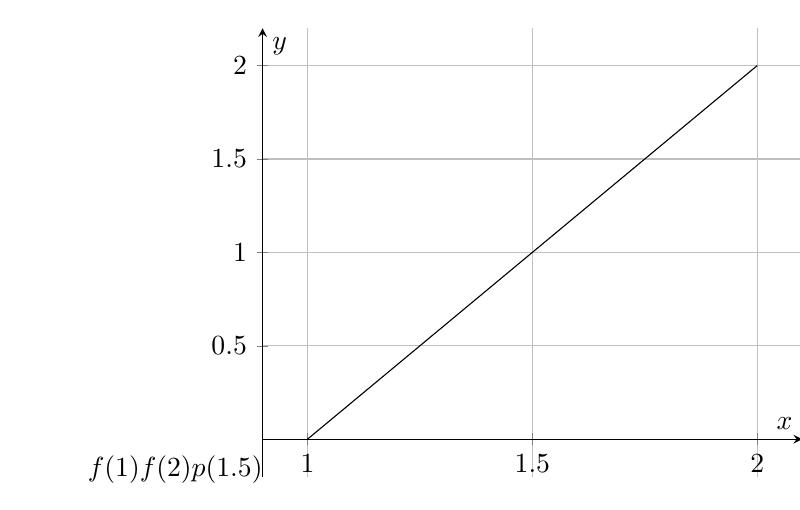
\begin{tikzpicture}
				\begin{axis}[
					axis lines=middle,
					xlabel=$x$,
					ylabel=$y$,
					enlargelimits,
					grid=major,
					legend pos=outer north east,
					%ymin=-0.3,
					%xmax=5.8,
					%xticklabels={,,},
					xtick={0, 1, 1.5, 2, 2.5},
					%yticklabels={,,},
					]
					\addplot[domain=1:2] {2*x - 2} node[left]{};
					\tikzPointUp{$f(1)$}{1,0}
					\tikzPointDown{$f(2)$}{2,2}
					\tikzPointDR{$p(1.5)$}{1.5,1}
					\legend{$p(x)$}
				\end{axis}
			\end{tikzpicture}
			\caption{Das Beispiel grafisch veranschaulicht.}
		\end{figure}
	}
	
	\sbreak
	\subsubsection{Lagrange-Basis} \label{sec:lagrange_basis}
	
	\sbreak
	\defi{ 
		\n
		Die Lagrange-Basis soll eine Möglichkeit sein, "schlaue" Basisfunktionen zu erstellen. \\
		Folgendermaßen wird sie berechnet: 
		\begin{align} 
	 		L_j = \prod_{i = 0; i \neq j}^{n-1} \frac{x - x_i}{x_j - x_i} 
	 	\end{align}
		Wenn man die $L_j$ nun als Basisfunktionen $g_0, \dots, g_{n-1}$ verwendet und das LGS lösen will, stellt man fest, dass die linke Matrix immer der Einheitsmatrix $\unitM$ entspricht und das Lösen des LGS trivial macht. Das liegt daran, dass die "schlauen" Basisfunktionen eben nur an der Stelle der jeweiligen Stützstelle $1$ beträgt und an allen anderen $0$.
		Ohne das LGS zu berechnen entsteht also die Interpolationspolynomfunktion 
		\begin{align} 
	 		p(x) = \sum_{j = 0}^{n-1}y_j \cdot L_j(x) 
	 	\end{align}
		Hier sehen wir, dass das Aufstellen der Funktion faktisch gar nichts kostet (bzw. $\bigO(n)$), das Auswerten der Interpolationsfunktion jedoch $\bigO(n^2)$!
	}
	
	\sbreak
	\bsp{
		\n
		Wir haben die Punktemenge von Stützstellen gegeben mit:
		\begin{align*}
			P: 
			\begin{Bmatrix}
				(0,1), (1,4), (3, -2)
			\end{Bmatrix}
		\end{align*}
		Wir möchten mithilfe von Lagrange-Basisfunktionen das Interpolationspolynom aufstellen:
		\begin{align*}
			L_0 &= \frac{(x - 1)(x - 3)}{(0 - 1)(0 - 3)} = \frac{(x - 1)(x - 3)}{3}\\
			L_1 &= \frac{(x - 0)(x - 3)}{(1 - 0)(1 - 3)} = \frac{x \cdot (x - 3)}{-2}\\
			L_2 &= \frac{(x - 0)(x - 1)}{(3 - 0)(3 - 1)} = \frac{x \cdot (x - 1)}{6}
		\end{align*}
		Jetzt noch die Interpolationsfunktion ausrechnen:
		\begin{align*}
			p(x) &= 1 \cdot L_0 + 4 \cdot L_1 -2 \cdot L_2 \\
				&= 1 \cdot \frac{(x - 1)(x - 3)}{3} + 4 \cdot \frac{x \cdot (x - 3)}{-2} - 2 \cdot \frac{x \cdot (x - 1)}{6} \\
				&= 1 + 5 \cdot x - 2 \cdot x^2
		\end{align*}
		\n 
		\begin{figure}[H]
			\centering
				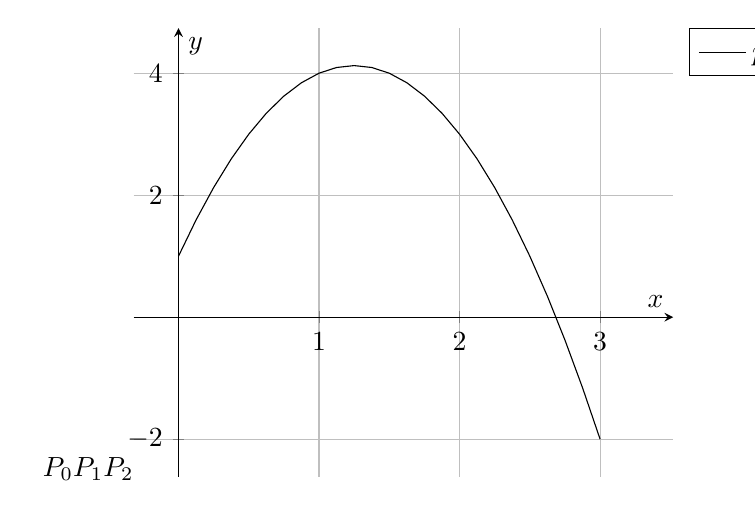
\begin{tikzpicture}
					\begin{axis}[
						axis lines=middle,
						xlabel=$x$,
						ylabel=$y$,
						enlargelimits,
						legend pos=outer north east,
						grid=major,
						xmax=3.2,
						%ymin=-0.3,
						%xmax=5.8,
						%xticklabels={,,},
						%yticklabels={,,},
						]
						\addplot[domain=0:3] {1 + 5*x^1 - 2*x^2} node[left]{};
						\tikzPointRight{$P_0$}{0,1}
						\tikzPointDR{$P_1$}{1,4}
						\tikzPointUR{$P_2$}{3,-2}
						\legend{$p(x)$}
					\end{axis}
				\end{tikzpicture}
			\caption{Das Beispiel grafisch veranschaulicht.}
		\end{figure}
	}

	\sbreak
	\wichtig{ \label{chap:polynomInterpolationEindeutigkeit}
		\n
		Ein Interpolationspolynom ist stets \fat{eindeutig}! Egal ob man die Standard Polynom Basisfunktionen, die Lagrange Basis oder so verwendet kommt zu einem Problem immer dasselbe Polynom raus. Auf Genauigkeit brauchen wir also keinen dieser Algorithmen untersuchen, jedoch aber die Anzahl an darstellbaren Polynomgraden (im Moment $n-1$ für $n$ Stützstellen). 
	}


	\newpage
% =========================================================	
	\subsubsection{Interpolation nach Newton} \label{chap:newtoninterpolation}
% =========================================================	
	
	\sbreak
	\defi{
		\n
		Die Interpolation nach Newton ist ein effizienterer Algorithmus, ein Interpolationspolynom analytisch auszurechnen, denn das Verfahren braucht für das Berechnen der Koeffizienten nur $\bigO(n^2)$ und das Auswerten der Funktion auch nur $\bigO(n)$.
	}

	\sbreak
	\methode{
		\n
		Wir definieren:
		\begin{align}
			c_{i,0} &= f(x_i) = y_i \\
			c_{i,k} &= \frac{c_{i+1,k-1} - c_{i,k-1}}{x_{i+k} - x_i}
		\end{align}
		Informeller ist folgendes:
		\begin{align} 
 			[\text{neu}]c = \frac{f\uleftDown - f\uleft}{x\uleftDiagonal - x\uleft} 
 		\end{align}
		Dabei sind die Richtungen immer in Relation zu der Stelle des zu ausrechnenden Wertes in der Tabelle angegeben. "ganzLinksUnten" meint, dass man in der Tabelle soweit nach ganz links unten zieht, bis man mit dem nächsten "Links-Unten-Move" nicht mehr in der rechten Seite der Tabelle wäre. Von dort aus nimmt man den x-Wert ganz links in derselben Zeile.
		\begin{table}[H]
			\label{table:newton}
			\centering
			\begin{tabular}{cc|cccc}
				\toprule
				$x_i$  & $i \setminus k$ & 0 & 1 & 2 & \dots \\ \midrule
				$x_0$ & $0$ & $c_{0,0}$ & $c_{0,1}$ & $c_{0,2}$ & \dots \\
				$x_1$ & $1$ & $c_{1,0}$ & $c_{1,1}$ & \mddots & \\
				$x_2$ & $2$ & $c_{2,0}$  & \mddots & & \\
				\vdots & & \mddots & & & \\
			\end{tabular}
			\caption{Tabelle zum Ausrechnen}
		\end{table}
		\noindent Wenn wir das fertig aufgestellt haben, können wir direkt alle Koeffizienten ablesen:
		\begin{align} 
			p(x) = c_{0,0} + c_{0,1} \cdot (x-x_0) + \dots + c_{0,n-1} \cdot \prod_{i=0}^{n-2}(x-x_i)
		\end{align}
		Unsere Koeffizienten sind also einfach die Werte der ersten Zeile der Tabelle.
	}

	\newpage
	\bsp{ \n 
		Wir haben:
		\begin{table}[H]
			\centering
			\begin{tabular}{cc|cccc}
				\toprule
				$x_i$  & $i \setminus k$ & 0 & 1 & 2 \\ \midrule
				$0$ & $0$ & $0$ & $c_{0,1}$ & $c_{0,2}$ \\
				$2$ & $1$ & $4$ & $c_{1,1}$ & \\
				$3$ & $2$ & $9$ & &
			\end{tabular}
		\end{table}%
		\begin{align*} 
 			c_{0,1} &= \frac{4 - 0}{2 - 0} = 2 \\
 			c_{1,1} &= \frac{9 - 4}{3 - 2} = 5 \\
			c_{0,2} &= \frac{5 - 2}{3 - 0} = 1 
		\end{align*}
		\begin{table}[H]
			\centering
			\begin{tabular}{cc|cccc}
				\toprule
				$x_i$  & $i \setminus k$ & 0 & 1 & 2 \\ \midrule
				$0$ & $0$ & $0$ & $2$ & $1$ \\
				$2$ & $1$ & $4$ & $5$ & \\
				$3$ & $2$ & $9$ & & \\
			\end{tabular}
		\end{table}
		Also kommt als Interpolationsfunktion folgendes heraus:
		\begin{align*} 
	 		p(x) &= c_{0,0} + c_{0,1} \cdot (x - x_0) + c_{0,2} \cdot (x - x_0)(x-x_1) \\
	 		&= 0 + 2 \cdot (x - 0) + 1 \cdot (x - 0)(x - 2) \\
	 		&= 0 + 2x + 1 \cdot x^2 - 2x \\
	 		&= x^2
	 	\end{align*}
		Würden wir hier die Punkte oben betrachten, sehen wir schon, dass es auf $x^2$ hinauslaufen wird.
	}

	\sbreak
	\defi{
		\n 
		Es ist vielleicht schon zu erkennen, aber wenn jetzt noch ein neuer Stützpunkt hinzugefügt werden soll, kann man diesen in der Tabelle einfach darunter schreiben und den neuen Koeffizienten relativ schnell ausrechnen. Dann muss nur noch das Ergebnis angepasst werden, indem ein weiteres Summenglied hinzugefügt wird und wir sind schon fertig. Das ist ein \fat{großer Vorteil} dieses Verfahrens.
	}

	\newpage
	\bsp{
		\n 
		Wir erweitern letztes Beispiel um einen weiteren Stützpunkt, und zwar mit $(-2, 4)$.
		\begin{table}[H]
			\centering
			\begin{tabular}{cc|ccccc}
				\toprule
				$x_i$  & $i \setminus k$ & 0 & 1 & 2 & 3
				\\ \midrule
				$0$ & $0$ & $0$ & $2$ & $1$ & $c_{0,3} = ?$\\
				$2$ & $1$ & $4$ & $5$ & $?$ &\\
				$3$ & $2$ & $9$ & $?$ & &\\
				$-2$ & $3$ & $4$ & & &
			\end{tabular}
		\end{table}
		\noindent Wir müssen die mit Fragezeichen markieren Stellen noch ausrechnen, um auf den neuen Koeffizienten $c_{0,3}$ schließen zu können.
		\begin{align*} 
			c_{2,1} &= \frac{4 - 9}{-2 - 3} = 1 \\
			c_{1,2} &= \frac{1 - 5}{-2 - 2} = 1 \\
			c_{0,3} &= \frac{1 - 1}{-2 - 0} = 0 = c_3
		\end{align*}
		Insgesamt sieht die Tabelle also folgendermaßen aus:
		\begin{table}[H]
			\centering
			\begin{tabular}{cc|ccccc}
				\toprule
				$x_i$  & $i \setminus k$ & 0 & 1 & 2 & 3
				\\ \midrule
				$0$ & $0$ & $0$ & $2$ & $1$ & $0$\\
				$2$ & $1$ & $4$ & $5$ & $1$ &\\
				$3$ & $2$ & $9$ & $1$ & &\\
				$-2$ & $3$ & $4$ & & &
			\end{tabular}
		\end{table}
		\noindent Jetzt noch die Interpolationsfunktion ausrechnen:
		\begin{align*} 
			p(x) &= c_{0,0} + c_{0,1} \cdot (x - x_0) + c_{0,2} \cdot (x - x_0)(x - x_1) + c_{0,3} \cdot (x - x_0)(x - x_1)(x - x_2)\\
			&= 0 + 2 \cdot (x - 0) + 1 \cdot (x - 0)(x - 2) + 0\\
			&= 0 + 2x + 1 \cdot x^2 - 2x \\
			&= x^2
		\end{align*}
		Das Ergebnis ist logisch, da der neue Punkt $(-2, 4)$ auch auf der Funktion $x^2$ liegt. Die Hinzunahme dieses Stützpunktes dürfte unser Ergebnis gar nicht abändern! Das können wir außerdem daher ablesen, dass der neu berechnete Koeffizient $0$ ist und damit keinen Einfluss auf die Ergebnisfunktion hat.
	}
	
	\newpage
% =========================================================	
	\subsubsection{Aitken-Neville}
% =========================================================	
	
	\defi{\n
		Dieses Verfahren dient dazu, ein Interpolationspolynom \fat{direkt an einer Stelle x auszuwerten}, obwohl wir das Polynom selbst nie ausgerechnet haben. Aitken-Neville rechnet das Polynom auch nicht direkt aus.
		\n
		Das machen wir, indem wir eine Tabelle ähnlich der bei Newton aufstellen:
	}
	
	\sbreak
	\methode{
		\begin{table}[H]
			\label{table:aitken}
			\centering
			\begin{tabular}{cc|cccc}
				\toprule
				$x_i$  & $i \setminus k$ & 0 & 1 & 2 & \dots \\ \midrule
				$x_0$ & $0$ & $p[0,0] = y_0$ & $p[0,1]$ & $p[0,2]$ & \dots \\
				$x_1$ & $1$ & $p[1,0] = y_1$ & $p[1,1]$ & \mddots & \\
				$x_2$ & $2$ & $p[2,0] = y_2$ & \mddots & & \\
				\vdots & & \mddots & & & \\
			\end{tabular}
			\caption{Berechnungstabelle für diese Methode}
		\end{table}
		mit der Formel: 
		\begin{align} 
			 p[i,k] := p[i, k-1] + \frac{x-x[i]}{x[i+k]-x[i]} \cdot (p[i+1, k-1] - p[i, k-1]) 
		\end{align}
		Die \fat{Lösung der Auswertung} steht in der Tabelle dann \fat{rechts oben!}
		\n
		Eine informelle Variante der Formel (mit derselben Notation wie bei Newton):
		\begin{align} 
	 		p_{\text{neu}} := p\uleft + \frac{x-x\uleft}{x\uleftDiagonal-x\uleft} \cdot (p\uleftDown - p\uleft) 
	 	\end{align}
	}

	\sbreak
	\defi{ \n
		Wie bei Newton (und in diesem Fach bei jedem Dreiecksschema) können wir wieder einfach neue Stützpunkte unten an die Tabelle einfügen und müssen nicht neu anfangen.\\
		Wenn wir das an einem Computer implementieren, können wir eine Laufzeit von $\bigO(n^2)$ herauslesen.
		Dieses Verfahren ist jedoch nur interessant, wenn man nur wenige Punkte auswerten will und die Funktion explizit nicht benötigt!
	}
	
	\newpage
	\bsp{ 
		\n
		Es seien die Stützpunkte einer unbekannten Funktion $f(x)$ gegeben:
		\begin{align*} 
 			f(0) = 0 \aae f(1) = 1 \aae f(2) = 4 
 		\end{align*}
		Wir möchten den Funktionswert an der Stelle $x = 0.5$ auswerten:
		\begin{table}[H]
			\label{table:aitkenBsp}
			\centering
			\begin{tabular}{cc|ccc}
				\toprule
				$x_i$  & $i \setminus k$ & 0 & 1 & 2 \\ \midrule
				$x_0 = 0$ & $0$ & $y_0 = 0$ & $p[0,1]$ & $p[0,2]$ \\
				$x_1 = 1$ & $1$ & $y_1 = 1$ & $p[1,1]$ & \\
				$x_2 = 2$ & $2$ & $y_2 = 4$ & & \\
			\end{tabular}
		\end{table}
		Ausrechnen der unbekannten Werte in der Tabelle:
		\begin{align*} 
			p_{\text{neu}} := p\uleft + \frac{x-x\uleft}{x\uleftDiagonal-x\uleft} \cdot (p\uleftDown - p\uleft) 
		\end{align*}
		\begin{align*} 
 			p[0,1] &= p[0, 0] + \frac{0.5 - x[0]}{x[1]-x[0]} \cdot (p[1, 0] - p[0, 0]) = \frac{1}{2} \\
			p[1,1] &= p[1, 0] + \frac{0.5 - x[1]}{x[2]-x[1]} \cdot (p[2, 0] - p[1, 0]) = -\frac{1}{2} \\
			p[0,2] &= p[0, 1] + \frac{0.5 - x[0]}{x[2]-x[0]} \cdot (p[1, 1] - p[0, 1]) = \frac{1}{4}
		\end{align*}
		Das Ergebnis ist also $f(0.5) = 0.25$, was auch Sinn ergibt, da unsere Stützpunkte recht eindeutig auf $f(x) = x^2$ hinweisen. Bei schwierigeren Stützpunkten wird Aitken-Neville aber ungenauer (genau so ungenau wie andere Polynominterpolation Methoden, siehe \ref{chap:polynomInterpolationEindeutigkeit}).
		%}
		%
		\n
		\begin{figure}[H]
			\centering
			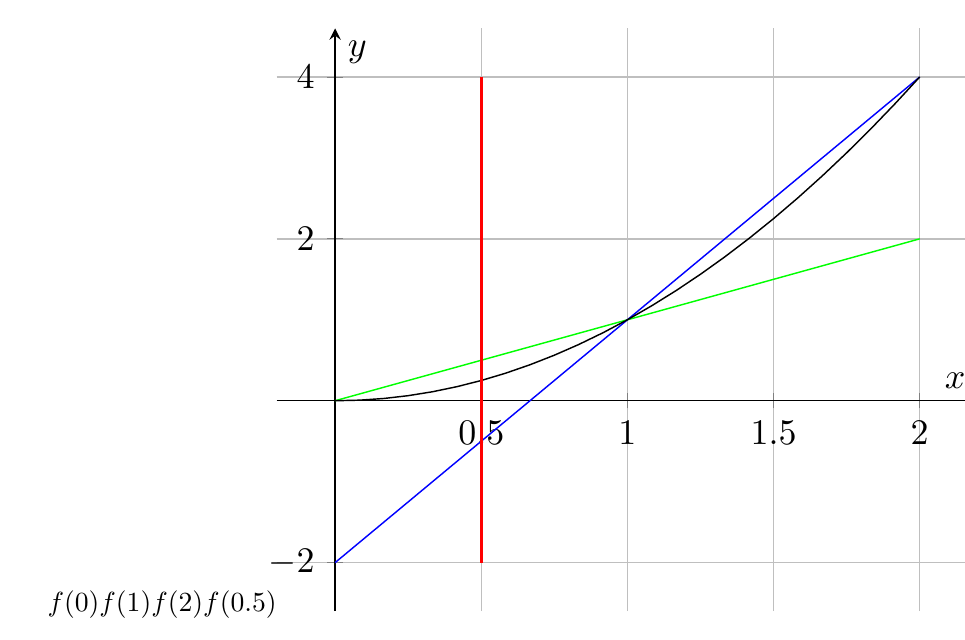
\begin{tikzpicture}[scale=1.3]
				\begin{axis}[
					axis lines=middle,
					xlabel=$x$,
					ylabel=$y$,
					enlargelimits,
					grid=major,
					legend pos=outer north east,
					%ymin=-0.3,
					%xmax=5.8,
					%xticklabels={,,},
					%yticklabels={,,},
					]
					\addplot[color=green, domain=0:2] {x} node[left]{};
					\addplot[color=blue, domain=0:2] {3*x-2} node[left]{};
					\addplot[domain=0:2] {x*x} node[left]{};
					\addplot[color=red, thick] coordinates {
						( 0.5, -2.0 )
						( 0.5, 4 )
					};
					\tikzPoint{60}{$f(0)$}{0,0}
					\tikzPointUp{$f(1)$}{1,1}
					\tikzPointLeft{$f(2)$}{2,4}
					\tikzPointDL{$f(0.5)$}{0.5,0.25}
					\legend{$p_{0,1}$, $p_{1,0}$, $p(x)$}
				\end{axis}
			\end{tikzpicture}
			\caption{Das Ergebnis des Beispiels grafisch. Interpolation erst einmal zwischen jeweils zwei der Punkte ($p[0,1]$ ist hierbei der Punkt bei $x=0.5$ der grünen Linie, $p[1,0]$ die blaue Linie).}
		\end{figure}
	}
	
	\lbreak
	\vertief{
		\n 
		Wenn man in der Aitken-Neville Formel das $x$ einfach als Variable lässt anstelle von einer bestimmten Stelle einzusetzen, wird das Ergebnis äquivalent zu der Interpolationsfunktion von Newton, Lagrange, \dots 
		\n 
		In diesem Fach behandeln wir Aitken-Neville aber so, wie wenn das nicht möglich wäre. Fragt mich nicht warum. \Laughey
	}
	
	\newpage
	\subsubsection{Fehlerabschätzung} \label{sec:interpolation_fehler}
	
	\methode{
		\n
		So kann man den Interpolationsfehler an einer Stelle $x$ abschätzen:
		\begin{align} 
	 		\abs{f(x) - p(x)} = \abs{\frac{f^{(n)}(\xi)}{(n)!} \cdot \prod_{k=0}^{n-1}(x-x_k)} 
	 	\end{align}
		mit $n$ Stützstellen und $\xi$ entspricht einem Wert im Interpolationsbereich (kommt aus dem Mittelwertsatz). Man wählt $\xi$ eigentlich immer so, dass der abgeschätzte Fehler maximal wird. Die Abschätzung des worst-case hat für uns die größte Aussagekraft.
		\n 
		$f^{(n)}$ steht hierbei für die $n$-te Ableitung von $f$.
	}
	

	\sbreak
	\bsp{
		\n
		Wir interpolieren eine Funktion mithilfe von $2$ Stützpunkten an den Stellen $1$ und $4$. Damit ist der Interpolationsbereich definiert mit $x \in [1, 4]$ und wir wollen den Fehler an der Stelle $x = 2$ abschätzen. %In der Aufgabenstellung sei gegeben, dass das größtmögliche $\xi$ gewählt werden soll, also $\xi = 4$.
		\n 
		Wir setzen in obige Formel ein:
		\begin{align*} 
			\abs{f(x) - p(x)} &= \abs{\frac{f^{(2)}(\xi)}{(2)!} \cdot \prod_{k=0}^{2-1}(x-x_k)}  \\
				&= \abs{\frac{f^{(2)}(\xi)}{(2)!} \cdot (2 - x_0)(2 - x_1)}
		\end{align*}
		Sei die zweite Ableitung gegeben, können wir das ganze ausrechnen:
		\begin{align*}
			f"(x) &= \frac{21}{2} \cdot x
		\end{align*}
		Da wir eine worst-case Abschätzung machen wollen, wählen wir $\xi \in [1, 4]$ so, dass die Fehlerabschätzung größtmöglich wird. Hier ist das offensichtlich mit $\xi = 4$ der Fall:
		\begin{align*}
			\abs{f(x) - p(x)} &= \abs{\frac{21 \cdot 4}{2 \cdot 2} \cdot (2 - 1)(2 - 4)}  \\
				&= \abs{21 \cdot 1 \cdot -2} \\
				&= 42
		\end{align*}
		%Da in der zweiten Ableitung kein $x$ mehr vorkommt ist in diesem Fall das $\xi$ völlig irrelevant, da egal wie wir es wählen, das Ergebnis bliebe gleich. \\
		(Dass 42 rauskommt ist kein Zufall \Cooley)
	}

	\newpage
	% =========================================================	
	\subsection{Runge-Effekt}
	% =========================================================
	
	\sbreak
	\defi{
		\n
		Wir haben uns noch nicht mit Problemen der Polynominterpolation beschäftigt. Ein klassisches Beispiel wäre der Runge Effekt.
		\n
		Der Runge Effekt tritt dann auf, wenn man sich mit der Polynominterpolation von Polynomen hohen Grads beschäftigt und äquidistante Stützstellen verwendet. Äquidistant bedeutet hierbei einfach nur, dass diese gleich verteilt sind bzw. der Abstand von jeder Stützstelle zu ihren Nachbarn gleich groß ist. Bisher dachten wir, je mehr Stützstellen wir hinzufügen, desto besser wird auch die Qualität des Interpolationspolynoms.
		\n
		Das ist nicht der Fall. Gerade die Ränder von Interpolationspolynomen mit vielen Stützstellen werden extrem ungenau, das nennen wir den Runge Effekt.
		\n 
		Folgende Erklärung: Wenn wir eine Funktion mit vielen äquidistanten Stützstellen haben, hat unser Interpolationspolynom zwangsläufig einen hohen Grad (ignorieren wir mal triviale Fälle). Wenn dieser hohe Grad informell aber nicht benötigt wird, kommt es zu Schwingungen, speziell an den Rändern des Interpolationsbereiches.
	}

	\picC{runge_pre.png}{0.75}{Interpolation mit wenigen Stützpunkten}
	\picC{runge_solution.png}{0.75}{Dasselbe Problem mit vielen Stützpunkten}
	
	\defi{
		\n 
		Welches der obigen Bilder zeigt die bessere Annäherung der Funktion (gestrichelte Linie) mithilfe von Polynominterpolation (durchgezogene Linie)?
		\n 
		Genau, das obere, welches deutlich weniger Stützpunkte nutzt\dots
	}
      % Polynominterpolation
	

	\newpage
	\subsection{Lineare Interpolation} \label{chap:linearInterpolation}
	
	\sbreak
	\defi{
		\n 
		Die lineare Interpolation ist denkbar einfach. Wir sollen ja eine Funktion finden, die durch alle Stützpunkte hindurchgeht. Also können wir doch benachbarte Stützpunkte einfach mit Geraden verbinden und fertig.
		\n 
		Das Ergebnis ist eine Sammlung an Teilfunktionen, deren Funktionsintervalle genau an den Rändern jeweils anknüpfen.
	}

	\sbreak
	\methode{
		\n 
		Zwischen zwei benachbarten Stützpunkten $(x_i, y_i)$ und $(x_{i+1}, y_{i+1})$ definieren wir eine lineare Verbindung mit
		\begin{align}
			p_i(x) = (x - x_i) \cdot \frac{y_{i+1} - y_i}{x_{i+1} - x_i} + y_i \quad \quad x \in [x_i, x_{i+1}]
		\end{align}
		Machen wir das für alle $i = 0, \dots, n-1$, erhalten wir all solche Geraden, welche wir durch die Intervall Definitionen aneinander "kleben" können.
	}

	\sbreak
	\bsp{
		\n 
		Wir haben die Stützpunkte $(0, 1)$, $(1, 3)$ und $(3, 0)$. Wir möchten diese stückweise linear interpolieren.
		Wir definieren unsere zwei Teilfunktionen mit obiger Methode:
		\begin{align*}
			p_0(x) &= (x - x_0) \cdot \frac{y_{1} - y_0}{x_{1} - x_0} + y_0 &&	x \in [x_0, x_{1}] \\
				&= (x - 0) \cdot \frac{3 - 1}{1 - 0} + 1 &&	x \in [0, 1] \\
				&= x \cdot 2 + 1 &&	x \in [0, 1] \\
				& &&\\
			p_1(x) &= (x - x_1) \cdot \frac{y_{2} - y_1}{x_{2} - x_1} + y_1 &&	x \in [x_1, x_{2}] \\
				&= (x - 1) \cdot \frac{0 - 3}{3 - 1} + 3 &&	x \in [1, 3] \\
				&= (x - 1) \cdot -\frac{3}{2} + 3 &&	x \in [1, 3] \\
				&= -\frac{3}{2}x + \frac{9}{2}  &&	x \in [1, 3]
		\end{align*}
		\newpage
		\noindent Insgesamt könnten wir unsere Interpolationsfunktion (unser Ergebnis nennt man so) also folgendermaßen definieren:
		\begin{align*}
			g(x) = 
			\begin{Bmatrix}
				p_0(x); & x\in[0;1[ \\
				p_1(x); & x\in[1;3] \\
			\end{Bmatrix}
		\end{align*}
		Das bedeutet nichts anderes als, wenn man ein bestimmtes $x$ in $g(x)$ einsetzt, die Teilfunktion (also $p_0$ oder $p_1$) ausgesucht wird, in welchem Intervall sich das $x$ befindet. Wenn man beispielsweise jetzt $g(2)$ ausrechnen möchte, wird die zweite Teilfunktion ausgesucht, da $2 \in [1;3]$ gilt. 
		\begin{align*}
			g(2) = p_1(2) = -\frac{3}{2} \cdot 2 + \frac{9}{2}
		\end{align*}
		Klar könnte man in der Definition von $g(x)$ oben noch $p_0(x)$ sowie $p_1(x)$ einsetzen aber das spare ich mir mal \Laughey.
		\n
		Grafisch sähe das dann so aus:
		\begin{figure}[H]
			\centering
				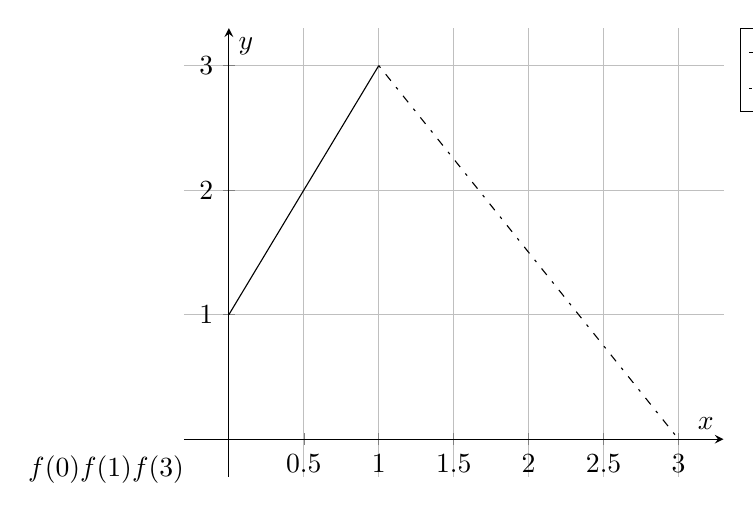
\begin{tikzpicture}
					\begin{axis}[
						axis lines=middle,
						xlabel=$x$,
						ylabel=$y$,
						enlargelimits,
						grid=major,
						cycle list name=color list,
						legend pos=outer north east,
						%ymin=-0.3,
						%xmax=5.8,
						%xticklabels={,,},
						%xtick={0, 1, 1.5, 2, 2.5},
						%yticklabels={,,},
						]
						\addplot[domain=0:1] {2*x + 1} node[left]{};
						\addplot[domain=1:3,dash pattern=on 1pt off 3pt on 3pt off 3pt] {-(3/2)*x + (9/2)} node[left]{};
						\tikzPointRight{$f(0)$}{0,1}
						\tikzPointRight{$f(1)$}{1,3}
						\tikzPointUp{$f(3)$}{3,0}
						\legend{$p_0(x)$, $p_1(x)$}
					\end{axis}
				\end{tikzpicture}
			\caption{Stückweise lineare Interpolation grafisch.}
		\end{figure}
	}

	\sbreak
	\wichtig{
		\n 
		Die erstellten Funktionen durch stückweise lineare Interpolation haben immer Knicke! Das bedeutet die Funktion ist nicht stetig differenzierbar!
	}
	       % Lineare Interpolation
	
	\newpage
% =========================================================	
	\subsection{Hermite Interpolation} \label{chap:hermite_interpolation}
% =========================================================
	
	\defi{
		\n 
		Ein Problem, welches wir mit einer Interpolationsfunktion bekommen könnten: Sie ist nicht stetig differenzierbar (wie stückweise lineare Interpolation, siehe \refChapter{chap:linearInterpolation}). 
		\n 
		Dieses Problem löst die Hermite Interpolation als netten Nebeneffekt, da sie für die Interpolation auch die Ableitung der Stützstellen einberechnet. Eigentlich ist sie "nur" eine genauere Interpolations Möglichkeit.
		\n 
		Schonmal gleich im Voraus, die Hermite Interpolation ist mit einer Laufzeit von $\bigO(n^3)$ aber relativ kostenaufwändig.
		\n 
		Mit der Standard Polynom Funktion dritten Grades
		\begin{align} 
 			p(t) = c_3 \cdot t^3 + c_2 \cdot t^2 + c_1 \cdot t + c_0 
 		\end{align}
 		und dessen Ableitung können wir ein LGS aufstellen und lösen. Also wir verwenden nicht nur die Position von den Stützpunkten, sondern auch deren Ableitungen. Im konkreten Hermite Fall zwei Stützstellen und deren Ableitungen, weswegen wir auf einen Grad von $3$ kommen.
	}
	
	\sbreak 
	\methode{
		\begin{itemize}
			\item LGS mithilfe von Stützstellen und deren Ableitung aufstellen.
			\item LGS lösen.
			\item Ergebnis des LGS in allgemeine Polynomfunktion einsetzen.
			\item Nach allen y und y' sortieren, also sodass da $y_0 \cdot \text{\qu{irgendwas}} + y_1 \cdot \text{\qu{irgendwas}} + \dots$ steht.
			\item Mithilfe von Koeffizientenvergleich auf die Basisfunktionen schließen, nach dem letzten Punkt entsprechen die "irgendwas" den Basisfunktionen.
			\item Hermite-Funktion (sortiert mit kubischen Basispolynomen):
			\begin{align} 
 				p(t) = y_0 \cdot H_0(t) + y_1 \cdot H_1(t) + y_0'\cdot H_2(t) + y_1' \cdot H_3(t) \quad\in [0;1] 
 			\end{align}
		\end{itemize}
	}
		
	\newpage
	\bsp{
		\n 
		Wir haben eine unbekannte Funktion $f(x)$ gegeben.\\
		Folgende Informationen seien über $f(x)$ bekannt:
		\begin{align*} 
 			f(0) = 0 \aae f(1) = 2 \aae f'(0) = 2 \aae f'(1) = 1 
 		\end{align*}
		Terme aufstellen (mithilfe der Funktion eines allg. Polynom dritten Grades):
		\begin{align*} 
 			f(t) &= c_3 \cdot t^3 + c_2 \cdot t^2 + c_1 \cdot t + c_0 \\
 			f(0) &= c_0 \shouldEq y_0 = 0 \\
 			f(1) &= c_3 + c_2 + c_1 + c_0 \shouldEq y_1 = 2 
 		\end{align*}
		Jetzt müssen wir in die Ableitung einsetzen:
		\begin{align*} 
 			f'(t) &= 3c_3 \cdot t^2 + 2c_2 \cdot t + c_1 \\
 			f'(0) &= c_1 \shouldEq y_0' = 2 \\
 			f'(1) &= 3\cdot c_3 + 2\cdot c_2 + c_1\shouldEq y_1' = 1 
 		\end{align*}
		Das entspricht folgender Vektor-Matrix-Schreibweise und damit LGS:
		\begin{align*}
			\begin{bmatrix}
				0 & 0 & 0 & 1 \\
				1 & 1 & 1 & 1 \\
				0 & 0 & 1 & 0 \\
				3 & 2 & 1 & 0 
			\end{bmatrix} \cdot 
			\nvector{
				c_3 \\ c_2 \\ c_1 \\ c_0
			} = 
			\nvector{
				y_0 \\ y_1 \\ y_0' \\ y_1'
			} = 
			\nvector{
				0 \\ 2 \\ 2 \\ 1
			}
		\end{align*}
		LGS lösen (Gauß-Elimination) ergibt:
		\begin{align*} 
 			c_0 = 0 \aae c_1 = 2 \aae c_2 = 1 \aae c_3 = -1 
 		\end{align*}
		Die Interpolationsfunktion entspricht also:
		\begin{align*} 
 			p(t) = -t^3 + t^2 + 2 t + 0 
 		\end{align*}
		Nach den Stützwerten und deren Ableitung sortieren, um auf die kubischen Basisfunktionen zu schließen wurde hier nicht (mehr) ausgeführt.
	%}
	%	
		\begin{figure}[H]
			\centering
			\begin{tikzpicture}
				\begin{axis}[
					axis lines=middle,
					xlabel=$x$,
					ylabel=$y$,
					enlargelimits,
					grid=major,
					legend pos=outer north east,
					]
					\addplot[domain=-0.5:1.5] {-1*x^3 + x^2 + 2*x} node[left]{};
					\tikzPointDR{$f(0)$}{0,0}
					\tikzPointDown{$f(1)$}{1,2}
					\tikzLineUp{dash pattern=on 1pt off 3pt on 3pt off 3pt}{$f'(0)$}{-0.5,-1.0}{0.5,1.0}
					\tikzLineUp{dash pattern=on 1pt off 3pt on 3pt off 3pt}{$f'(1)$}{0.5,1.5}{1.5,2.5}
					\legend{Interpolationsfunktion}
				\end{axis}
			\end{tikzpicture}
			\caption{Obige Hermite-Interpolation grafisch. Wir verwenden nicht nur die Position der zwei Stützstellen, sondern auch deren Ableitung (hier als kurze gepunktete Linie eingezeichnet).}
		\end{figure}
	}

	\sbreak
	\methode{
		\n
		Aus obigen Beispiel können wir eine neue Formel herleiten. Für zwei Stützstellen an den Positionen $x_0 = 0$, $x_1 = 1$ und deren Ableitungen entspricht das LGS:
		\begin{align}
			\begin{bmatrix}
				3 & 2 & 1 & 0 \\
				1 & 1 & 1 & 1 \\
				0 & 0 & 1 & 0 \\
				0 & 0 & 0 & 1
			\end{bmatrix} \cdot 
			\nvector{
				c_3 \\ c_2 \\ c_1 \\ c_0
			} = 
			\nvector{
				y_1' \\ y_1 \\ y_0' \\ y_0
			}
		\end{align}
		Die berechneten $c_0$ bis $c_3$ können wir dann in unser Schema einsetzen
		\begin{align*}
			p(t) = c_3 \cdot t^3 + c_2 \cdot t^2 + c_1 \cdot t + c_0 
		\end{align*}
		und erhalten damit unser Ergebnis.
	}


	\newpage
	\vertief{
		\n 
		Den letzten Methodenblock können wir natürlich jetzt etwas optimieren, da er immer gleich bleibt.
		\n 
		LR Zerlegung wollt ihr? Kein Problem! Ich erspar euch den langen Rechenweg, Fakt ist das Ergebnis entspricht
		\begin{align*}
			L = 
			\begin{bmatrix}
				1 & 0 & 0 & 0 \\
				\nicefrac{1}{3} & 1 & 0 & 0 \\
				0 & 0 & 1 & 0 \\
				0 & 0 & 0 & 1
			\end{bmatrix}
			\quad \quad
			R = 
			\begin{bmatrix}
				3 & 2 & 1 & 0 \\
				0 & \nicefrac{1}{3} & \nicefrac{2}{3} & 1 \\
				0 & 0 & 1 & 0 \\
				0 & 0 & 0 & 1 
			\end{bmatrix}
		\end{align*}
		Jetzt könnt ihr einfach das und euer Wissen aus \refChapter{chap:lr_zerlegung} nutzen um so schneller Hermite Interpolationen durchzuführen. Für die Laufzeit eines Computerprogrammes hilft das natürlich herzlich wenig.
		\n 
		Die Zahlen der QR-Zerlegung sind leider weniger hübsch, sonst würde ich sie hier auch aufführen.
		\n 
		Um obige Korrektheit zu überprüfen, rechnen wir einfach die letzte Beispielbox mithilfe von LR Zerlegung.
		Zunächst müssen wir dafür $Ly = b$ lösen, also
		\begin{align*}
			\begin{bmatrix}
				1 & 0 & 0 & 0 \\
				\nicefrac{1}{3} & 1 & 0 & 0 \\
				0 & 0 & 1 & 0 \\
				0 & 0 & 0 & 1
			\end{bmatrix} \cdot y = 
			\nvector{
				1 \\ 2 \\ 2 \\ 0
			}
		\end{align*}
		Das Zwischenergebnis (hier ungünstig $y$ genannt, obwohl unsere $y$-Koordination auch den Namen haben) ist nach Gauß:
		\begin{align*}
			y = 
			\nvector{
				1 \\ \nicefrac{5}{3} \\ 2 \\ 0
			}
		\end{align*}
		Jetzt noch $Rx = y$ berechnen, wobei $x$ in dem Fall unseren $c_0$ bis $c_3$ entsprechen:
		\begin{align*}
			\begin{bmatrix}
				3 & 2 & 1 & 0 \\
				0 & \nicefrac{1}{3} & \nicefrac{2}{3} & 1 \\
				0 & 0 & 1 & 0 \\
				0 & 0 & 0 & 1 
			\end{bmatrix} \cdot
			\nvector{
				c_3 \\ c_2 \\ c_1 \\ c_0
			} = 
			\nvector{
				1 \\ \nicefrac{5}{3} \\ 2 \\ 0
			}
		\end{align*}
		Wenn man das mit Gauß berechnet, kommt in der Tat 
		\begin{align*} 
			c_0 = 0 \aae c_1 = 2 \aae c_2 = 1 \aae c_3 = -1 
		\end{align*}
		wie bei obiger Beispielbox heraus.
	}
		
	\newpage
	\defi{ \label{sec:intervall_transformation} %\fat{Transformation von Intervallen} 
		\n
		Kubische Polynome nennt man übrigens ganzrationale Polynome dritten Grades.
		\n 
		Das schöne bei der Hermite Interpolation ist es, dass man die kubischen Basisfunktionen für jeden (Interpolations-)Bereich derselben Funktion immer wiederverwenden kann und nicht mehr auszurechnen ist. Damit dies funktioniert müssen wir lediglich das neue Intervall (=Interpolationsbereich) auf das Intervall abbilden, in dem wir die Basisfunktionen ausgerechnet haben.
		\n 
		Wir rechnen also die kubischen Basisfunktionen immer im Intervall $[0,1]$ aus und müssen nur noch beliebige andere Intervalle, die wir ausrechnen wollen dahin transformieren.
		\n 
		Formal ausgedrückt müssen wir das neue (hier allgemeine) Intervall $[x_i, x_{i+1}]$ auf das vorherige $t \in [0;1]$ abbilden.
		\n 
		Das geht mit folgender Funktion: 
		\begin{align} 
 			t_i(x) := \frac{x-x_i}{x_{i+1} - x_i} \in [0;1] = \frac{x-x_i}{h_i} \in [0;1]
 		\end{align}
		Informell ist $h_i$ die Länge des Intervalls.
		\n 
		Wenn wir die transformierte (also auf das allg. Intervall abgebildete) Funktion ableiten wollen, müssen wir die Kettenregel berücksichtigen.
		\begin{align}
 			\frac{\d}{\d{x}}(f(t_i(x))) = \frac{\d}{\d{t}}(f(t_i(x))) \cdot \frac{\d t}{\d x} = \frac{\d}{\d t}(f(t_i(x)))\cdot \frac{1}{x_{i+1} - x_i} 
 		\end{align}
		Dadurch wird das sogenannte "kubische Teilpolynom" $p_i(t(x))$ auch noch folgendermaßen erweitert: Bei den Summanden der Ableitungen kommt der Faktor $h_i$ hinzu, weil dort bei der Ableitung sonst ein $\frac{1}{h_i}$ auftauchen würde, welche die Interpolation verfälschen würde. 
		\n 
		Damit haben wir die Formel für eine beliebige Hermite-Funktion:
		\begin{align} 
 			p_i(t_i(x)) = y_i\cdot H_0(t_i(x))+y_{i+1}\cdot H_1(t_i(x))+h_i\cdot y_i'\cdot H_2(t_i(x))+h_i\cdot y_{i+1}'\cdot H_3(t_i(x)). 
 		\end{align}
	}

	\newpage
	\bsp{
		\n 
		Wir wollen das Intervall $[3, 4]$ auf das Intervall $[0, 1]$ transformieren. Wir müssen also die Transformation nach obigem Schema aufstellen:
		\begin{align*}
			t(x) &= \frac{x - 3}{4 - 3} \\
				&= \frac{x - 3}{1}
		\end{align*}
		Jetzt müssen wir nur schreiben, dass $x \in [3,4]$ gilt und wir sind fertig, $t(x) \in [0,1]$ wie wir es wollten.
	}

	\sbreak
	\vertief{
		\n 
		Die Formel aus dem letzten Erklärblock ist um auf $[0, 1]$ zu transformieren. Wir können das natürlich für beliebige Intervalle ausbauen. Nützlich wenn wir beispielsweise die kubischen Basisfunktionen gar nicht für das Intervall $[0,1]$ ausrechnen können (warum auch immer).
		\n 
		Wenn wir ein beliebiges Intervall $[a, b]$ auf ein anderes beliebiges Intervall $[c, d]$ transformieren wollen, bilden wir folgende Transformationfunktion:
		\begin{align*}
			h_\text{ab} :&= b - a \\
			h_\text{cd} :&= d - c \\
			t(x) :&= \frac{x}{\nicefrac{h_\text{ab}}{h_\text{cd}}} + \l( c - \frac{a}{\nicefrac{h_\text{ab}}{h_\text{cd}}} \r) \\
			&= \frac{x \cdot h_\text{cd}}{h_\text{ab}} + \l( c - \frac{a \cdot h_\text{cd}}{h_\text{ab}} \r)
		\end{align*}
	}

	\sbreak
	\bsp{
		\n 
		Wir wollen das Intervall $[2,4]$ auf $[8, 14]$ transformieren. Wir nutzen obige Formel:
		\begin{align*}
			h_\text{ab} &= 4 - 2 = 2 \\
			h_\text{cd} &= 14 - 8 = 6 \\
			t(x) &= \frac{x \cdot 6}{2} + \l( 8 - \frac{2 \cdot 6}{2} \r) \\
				&= 3x + 2
		\end{align*}
		Und fertig \Laughey.
	}
	
		
	\newpage
	\subsection{Interpolation mit Splines}
	\label{chap:splines}
	
	\defi{
		\n 
		Die Interpolation mit Splines ist eine stückweise Interpolation. Sprich wir unterteilen den zu interpolierenden Bereich in diesem Fall bei jedem Stützpunkt, der sich nicht am Rand befindet. Jeder Bereich bildet hier ein sogenanntes "Spline".
		\n 
		Bei der Interpolation mit Splines wollen wir den gleichen Polynomgrad wie bei der Hermite-Interpolation erreichen, nur dass wir keine Ableitungen zur Verfügung haben. Aus diesem Grund verwenden wir als zusätzliche Bedingung, dass die Verknüpfungsstellen zwischen 2 Polynomen sowohl in der ersten als auch in der 2. Ableitung übereinstimmen. Diese Eigenschaft nennt man C2--Stetigkeit.
		\n
		Dies generiert 2 weitere Bedingungen, fehlen noch zwei, um auf den gewünschten Grad zu gelangen. Wir nehmen deshalb die Ableitungen an den Rändern, um die letzten Gleichungen zu erhalten.
		%Vorstellbar ist diese Vorgehensweise mithilfe einer Straklatte.
		%Man interpoliert gegebene Stützstellen mit Hilfe von stückweise stetiger Polynome (Splines genannt).
		}
	
	\lbreak
	\methode{
		\n 
		Mit 
		\begin{align*} 
 			x_{i+1} - x_i = h := \frac{x_n - x_0}{n}\aae i = 0,1,\dots,n-1 
 		\end{align*}
		Löse das System
		\begin{align}
			\begin{bmatrix}
				4 & 1 \\
				1 & 4 & \ddots\\
				  & \ddots & \ddots & 1\\
				  &   & 1 & 4
			\end{bmatrix} \cdot
			\nvector{
				y_1' \\ y_2' \\ \vdots \\ y_{n-2}' \\ y_{n-1}'
			}
			 = \frac{3}{h} \cdot
			\nvector{
				y_2 - y_0 \\
				y_3 - y_1 \\
				\vdots \\
				y_{n-1} - y_{n-3} \\
				y_n - y_{n-2}
			} - 
			\nvector{
				y_0' \\ 0 \\ \vdots \\ 0 \\ y_n'
			}
		\end{align}
		Bestimme mithilfe dieser Gleichung die Ableitungen aller Stützwerte außer den an den Rändern. Dann hat man alle Informationen, um für jedes Paar benachbarter Stützstellen die entsprechenden Hermite-Funktionen aufzustellen.
		\n 
		Für jedes Spline muss eine Transformationsfunktion aufgestellt werden, um die Intervalle zu normieren (siehe \refChapter{sec:intervall_transformation}). Danach kann man die Spline-Funktion definieren, die alle Splines vereinigt.
		\n
		Aufgrund dieser Tri-diagonalmatrix (nennt man so) ist die Laufzeit von Splines in $\bigO(n)$.
		}
	
	\sbreak
	\bsp{ Beispiel von oben erweitert:
		\begin{align*} 
 			f(0) = 0 \aae f(1) = 2 \aae f(2) = 4 \aae f(3) = 8 
 		\end{align*}
		Die Ableitung an den Rändern sei vorgegeben: 
		\begin{align*}
			f'(0) = 2 \aae f'(3) = 4
		\end{align*}
		Wir haben also 3 Splines mit einer Länge von eins ($h=1$).\\
		In die obige Formel einsetzen, um die restlichen zwei Ableitungen zu approximieren:
		\begin{align*}
			\begin{bmatrix}
				4 & 1 \\
				1 & 4
			\end{bmatrix} \cdot
			\nvector{
				y_1' \\ y_2'
			} &= \frac{3}{1} \cdot
			\begin{bmatrix}
				4 - 0 \\
				8 - 2
			\end{bmatrix} - 
			\nvector{
				2 \\ 4
			} \\
			\Longrightarrow
			\begin{bmatrix}
				4 & 1 \\
				1 & 4
			\end{bmatrix} \cdot
			\nvector{
				y_1' \\ y_2'
			} &= 
			\begin{bmatrix}
				12 - 2 \\
				18 - 4
			\end{bmatrix} = 
			\nvector{
				10 \\
				14
			}
		\end{align*}
		Dies entspricht einem LGS; die Lösung mithilfe von Gauß ist:
		\begin{align*} 
 			y_1' = \frac{26}{15} \aae y_2' = \frac{46}{15} 
 		\end{align*}
		Damit lässt sich dann mithilfe der kubischen Basispolynome von Hermite die Spline-Funktion aufstellen, die alle drei Splines vereint. Dafür müssen wir unter anderem noch die $t$-Funktionen setzen. Beispiel dafür folgt noch.
	}
	
	\lbreak
	\wichtig{ \n 
		Ein paar wichtige Dinge zu Splines: \\
		Wenn sich ein Stützpunkt ändert, wirkt sich das immer nur lokal auf einen kleinen Bereich der Kurve aus (halt nur ein bis zwei Splines), der Großteil der Kurve bleibt unverändert. \\
		Außerdem sind Spline Kurven so konstruiert, das sie möglichst glatt durch die Stützstellen laufen, da die Krümmung der Gesamtfunktion minimiert wird.
		\n 
		Starke Oszillationen wie bei Polynominterpolation hohen Grades (sprich Runge-Effekt) können nicht auftreten!
	}

	\newpage
	\bsp{ \n 
		Wir haben folgende Stützpunkte über eine unbekannte Funktion $f(x)$ gegeben und alle fehlenden Ableitungen nach der eingeführten Formel korrekt ausgerechnet:
		\begin{table}[H]
			\label{table:splinebsp}
			\centering
			\begin{tabular}{ccccc}
				\toprule
				$i$ 	& 0 	& 1 	& 2 	& 3 \\ \midrule
				$x_i$	& $-2$  	& 0 	& 2 	& 4 \\
				$y_i$	& 12 	& 4 	& 6    	& 3    \\
				$y'_i$  & $-4$    & $0.5$   & $-1$    & 1    \\
				\bottomrule
			\end{tabular}
			\caption{Alle Informationen als Tabelle}
		\end{table}
		\noindent Da wir vier Stützpunkte (an den Stellen $-2$, $0$, $2$ und $4$) haben, erhalten wir drei Splines. Deren Intervall ist in allen Fällen zwei lang (von $-2$ bis $0$ \dots).
		\n 
		Gegeben sei außerdem, dass die kubischen Basispolynome der unbekannten Funktion $f(x)$ im Intervall $[0;1]$ schon korrekt ausgerechnet worden sind.
		\n 
		Wir definieren unsere Spline-Funktion mit allen drei Splines:
		\begin{align*}
			s(x) = 
			\begin{Bmatrix}
				p_0(t_0(x)); & x\in[-2;0[ \\
				p_1(t_1(x)); & x\in[0;2[\\
				p_2(t_2(x)); & x\in[2;4]
			\end{Bmatrix}
		\end{align*}
		Die einzelnen $p$-Funktionen sind die einzelnen Splines und damit Hermite-Funktionen (die wir noch definieren müssen). Erst einmal müssen wir jetzt aber die Transformationsfunktionen $t_0(x), t_1(x)$ und $t_2(x)$ definieren, die das Intervall des jeweiligen Splines nach $[0;1]$ transformiert (weil dort die kubischen Basispolynome schon ausgerechnet worden sind).
		\n 
		Fangen wir vorne an:
		\begin{align*} 
 			&&&t_i(x) := \frac{x - x_i}{x_{i+1} - x_i} \\
			t_0(x) &= \frac{x + 2}{2} && x\in [-2;0] && t_0(x) \in [0;1] \\
			t_1(x) &= \frac{x}{2} && x\in [0;2] && t_1(x) \in [0;1] \\
			t_2(x) &= \frac{x - 2}{2} && x\in [2;4] && t_2(x) \in [0;1] 
 		\end{align*} \n
		Jetzt müssen wir noch die einzelnen Splines definieren. Wir nutzen obige allgemeine Hermite-Funktion:
		\begin{align*} 
 			p_i(t_i(x)) &= y_i \cdot H_0(t_i(x)) + y_{i+1} \cdot H_1(t_i(x)) + h_i \cdot y_i' \cdot H_2(t_i(x)) + h_i \cdot y_{i+1}' \cdot H_3(t_i(x))
 		\end{align*}
		Jetzt müssen wir nur noch aus unserer Tabelle die Werte einsetzen:
		\begin{align*} 
 			p_0(t_0(x)) &= y_0\cdot H_0(t_0(x))+y_{1}\cdot H_1(t_0(x))+h_0\cdot y_0'\cdot H_2(t_0(x))+h_0\cdot y_{1}'\cdot H_3(t_0(x)) \\
			&= 12\cdot H_0(t_0(x))+ 4\cdot H_1(t_0(x))+2\cdot (-4)\cdot H_2(t_0(x))+2\cdot \frac{1}{2}\cdot H_3(t_0(x)) 
 		\end{align*}
		Der Rest geht analog:
		\begin{align*} 
 			p_1(t_1(x)) &= 4\cdot H_0(t_1(x))+ 6\cdot H_1(t_1(x))+2\cdot \frac{1}{2}\cdot H_2(t_1(x))+2\cdot (-1)\cdot H_3(t_1(x)) \\
			p_2(t_2(x)) &= 6\cdot H_0(t_2(x))+ 3\cdot H_1(t_2(x))+2\cdot (-1)\cdot H_2(t_2(x))+2\cdot 1\cdot H_3(t_2(x)) 
 		\end{align*}
		Wir definieren mit obigen Hermite-Funktionen unsere fertige Spline-Funktion:
		\begin{align*}
			s(x) = 
			\begin{Bmatrix}
				p_0(t_0(x)); & x\in[-2;0[; & t_0(x) = \nicefrac{(x+2)}{2}\\
				p_1(t_1(x)); & x\in[0;2[;  & t_1(x) = \nicefrac{x}{2}\\
				p_2(t_2(x)); & x\in[2;4];  & t_2(x) = \nicefrac{(x-2)}{2}
			\end{Bmatrix}
		\end{align*}
	}
	
	\sbreak
	\defi{ \n 
		Ihr fragt euch sicher, warum wir oben als Randbedingung Ableitungen zur Verfügung haben, wenn die Idee doch eigentlich ist, keine zu benötigen. 
		\\ Die Antwort ist einfach: Dadurch, dass sich eine Änderung nur lokal auswirkt und in der Praxis die Interpolationsbereiche riesig sind, interessiert es uns nicht so sehr, wenn die Ränder der Interpolation ungenau sind. 
		\n 
		Also wir brauchen die Randableitungen dann doch nicht mehr, wir setzen sie einfach auf $0$. Sie verfälschen zwar dadurch unsere Ergebnisse (gerade an den Rändern), aber nicht viel. Bei einer niedrigen Spline Anzahl wäre das natürlich fataler.
		\n 
		Wie zur Hölle kommt man auf das Gleichungssystem, welches man für Splines verwendet\dots?
	}

	\newpage
	\vertief{ \fat{Spline-Interpolation Herleitung:} \n 
		Wir stellen wieder nach dem Hermite-Ansatz unsere Interpolationsfunktionen auf:
		\begin{align*} 
 			p_i(t_i(x)) = y_i \cdot H_0(t_i(x)) + y_{i+1} \cdot H_1(t_i(x)) + h \cdot y_i' \cdot H_2(t_i(x)) + h \cdot y_{i+1}' \cdot H_3(t_i(x)) 
 		\end{align*}
		Dafür benötigen wir wieder obige Transformationsfunktion und die Kettenregel, die schon oben eingebaut ist. 
		\n 
		Nun können wir alle $y_i$ bestimmen, indem wir die letzte Bedingung der C2-Stetigkeit nutzen. Wir setzen einfach die zweite Ableitung der Funktionen $p_i(t(x) = 1)$ und $p_{i+1}(t(x) = 0)$ an den Klebestellen gleich.
		\begin{align*} 
 			p_i"(t=1) = p_{i+1}"(t = 0) \aae i = 0, 1, \dots, n - 2 
 		\end{align*}
		Durch zweimaliges Ableiten der Basispolynome erhält man mit Kettenregel den Faktor $\nicefrac{1}{h^2}$, also:
		\begin{align*} 
 			&\frac{1}{h^2} \cdot [y_i \cdot H_0"(1) + y_{i+1} \cdot H_1"(1) + h \cdot y_i' \cdot H_2"(1) + h \cdot y_{i+1}' \cdot H_3"(1)] \\
 			= &\frac{1}{h^2} \cdot [y_{i+1} \cdot H_0"(0) + y_{i+2} \cdot H_1"(0) + h \cdot y_{i+1}' \cdot H_2"(0) + h \cdot y_{i+2}' \cdot H_3"(0)] 
 		\end{align*}
		Jetzt sortieren wir $y'$ auf die linke und $y$ auf die rechte Seite:
		\begin{align*} 
 			&\frac{h}{h^2} \cdot [y_i' \cdot H_2"(1) + y_{i+1}' \cdot (H_3"(1) - H_2"(0)) - y_{i+2}' \cdot H_3"(0)] \\
 			= &\frac{1}{h^2} \cdot [- y_{i} \cdot H_0"(1) + y_{i+1} \cdot (-H_1"(1) + H_0"(0)) + y_{i+2} \cdot H_1"(0)] 
 		\end{align*}
		Wenn wir hier nun unsere kubischen Basisfunktionen $H_i"$ mit $i = 0, \cdots, n-2$ einsetzen, kommen wir zwangsläufig auf:
		\begin{align*} 
 			[y_i' + 4y'_{i+1} + y'_{i+2}] = \frac{3}{h} \cdot [y_{i+2} - y_i] 
 		\end{align*}
		Und daraus können wir dann obiges Gleichungssystem ableiten:
		\begin{align*}
			\begin{bmatrix}
				4 & 1 \\
				1 & 4 & \ddots\\
				& \ddots & \ddots & 1\\
				&   & 1 & 4
			\end{bmatrix} \cdot
			\nvector{
				y_1' \\ y_2' \\ \vdots \\ y_{n-2}' \\ y_{n-1}'
			}
			= \frac{3}{h} \cdot
			\nvector{
				y_2 - y_0 \\
				y_3 - y_1 \\
				\vdots \\
				y_{n-1} - y_{n-3} \\
				y_n - y_{n-2}
			} - 
			\nvector{
				y_0' \\ 0 \\ \vdots \\ 0 \\ y_n'
			}
		\end{align*}
	}
		% Hermite + Splines

% ---------------------------------------------------------------------------
% Fourier
% ---------------------------------------------------------------------------
	
\newpage
% =========================================================	
\section{Komplexe Zahlen} \label{chap:komplexeZahlen}
% =========================================================

\defi{
	\n 
	Komplexe Zahlen $z \in \complexes$ bestehen aus einem \fat{Realteil} und einem \fat{Imaginärteil}.
	Hier sind kurz und knapp alle wichtigen Fakten in Stichpunkten zusammengefasst.
	\begin{itemize}
		\item $z = x + iy$
		\item $x = \realPart(z) \aae y = \imaginaryPart(z)$
		\item $i = \sqrt{-1}$
		\item $\compl{z} = x - iy$ \quad(komplex konjugiertes)
		\item $\compl{z \cdot w} = \compl{z} \cdot \compl{w}$
		\item $\abs{z} = \sqrt{\realPart(z)^2 + \imaginaryPart(z)^2} = \sqrt{z \cdot \compl{z}}$
		\item Euler-Formel: $e^{i\cdot m} = \cos(m) + i \cdot \sin(m)$
		\item $ e^z = e^{x + iy} = e^x (\cos(y) + i \cdot \sin(y))$
		\item $z_1 + z_2 = (x_1 + x_2) + i \cdot (y_1 + y_2)$
		\item $z_1 - z_2 = (x_1 - x_2) + i \cdot (y_1 - y_2)$
		\item $z_1 \cdot z_2 = (x_1 x_2 - y_1 y_2) + i \cdot (x_1 y_2 + x_2 y_1)$
	\end{itemize}
}

\bsp{
	\begin{align*}
	a = & 3 + 4i; \quad b = 5 + 3i \\
	\\
	\compl{a} &= 3 - 4i \\
	\\
	\realPart(a) &= 3 \\
	\imaginaryPart(a) &= 4 \quad \text{(nicht $4i$ \;!!!)} \\
	\\
	\abs{a} &= \sqrt{3^2 + 4^2} \\
		&= 5
	\end{align*}
	\n
	\begin{align*}
	e^a &= e^{3 + 4i} \\
		&= e^3 \cdot \l(\cos(4) + i \cdot \sin(4)\r)\\
	\\
	c &= a + b \\
		&= 8 + 7i \\
	\\
	d &= a \cdot b \\
		&= 3 \cdot 5 + 3 \cdot 3i + 4i \cdot 5 + 4i \cdot 3i \\
		&= (15 - 12) + (9 + 20)i \\
		&= 3 + 29i
	\end{align*}
}            % Komplexe Zahlen
	
	\newpage
% =========================================================	
	\section{Frequenzanalyse} \label{chap:Frequenzanalyse}
% =========================================================
	
	\defi{
		\n 
		Trigonometrische Funktionen (aka solche, die Operationen wie $\sin()$ verwenden), besitzen immer eine Amplitude und eine Frequenz. Einige Probleme in der Praxis (wie z.B. Soundwellen) basieren auf Signalen, die man in ihre einzelnen Frequenzen auftrennen möchte. Solche Signale nimmt man als Summen trigonometrischer Funktionen an und lassen sich oft anschaulich durch ihr "Spektrum" darstellen.
	}

	\sbreak
	\bsp{
		\n
		Gegeben sei folgende "Grundfrequenz":
		\begin{align*} 
 			f(x) = \sum_{k=0}^{\infty}c_k \cdot \cos(kx) 
 		\end{align*}
 		Damit lassen sich alle Signale darstellen, die nur aus Kosinus Überlagerungen bestehen. In dem Fall würde ein Signal, welches nur aus der normalen Kosinusfunktion besteht, ausschließlich das Spektrum $k = 1$ aufweisen. Eine gerade Linie als Signal hätte das Spektrum: $k = 0$.
 		\n 
 		Also sind die unterschiedlichen $k$ die unterschiedlichen Frequenzen, $c_k$ beschreibt den Gewichtungskoeffizienten. Bei der Frequenzanalyse ist das äquivalent zu der Amplitude der jeweiligen Frequenz. Also der normale Kosinus hat nur die Frequenz $k=1$ mit einer Amplitude von $c_k = 1$, da der Kosinus zwischen Eins und $-1$ schwingt.
		\n %ewpage
		Im Folgenden ein paar Beispiele von Schwingungen und ihren Frequenzspektren:
		\n
		$\cos(x)$: \\
		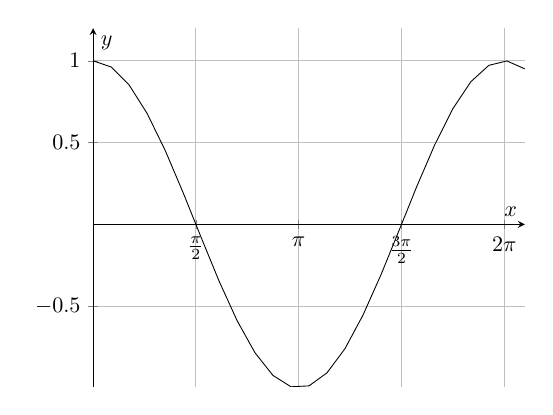
\begin{tikzpicture}[yscale=0.8, xscale=0.8]
					\begin{axis}[ 
						xtick={-3.14159, -1.5708, 0,1.5708,3.14159,4.7123889, 6.28318},
						xticklabels={$-\pi$, $-\frac{\pi}{2}$, $0$,$\frac{\pi}{2}$,$\pi$,$\frac{3\pi}{2}$,$2\pi$},
						axis lines=middle,
						ymax=1.2,
						grid=major,
						xlabel=$x$,
						ylabel=$y$,
						]
						\addplot[domain=0:2.1*pi] {cos(deg(x))} node[left]{};
					\end{axis}
				\end{tikzpicture}%
		\qquad
		\begin{tikzpicture}[yscale=0.8, xscale=0.8]
			\begin{axis}[
				axis lines=middle,
				xlabel=$k$,
				ylabel=$c_k$,
				ymin=0,
				%grid=major,
				ymax=1,
				xtick={0, 1, 2, 3, 4, 5, 6},
				xticklabels={0, 1, 2, 3, 4, 5, 6},
				enlargelimits,
				]
				\addplot[domain=0:6] {0} node[left]{};
				\tikzMegaFatLine{}{1,0}{1,1}
			\end{axis}
		\end{tikzpicture}%
		\newpage
		$0.5 \cdot \cos(x) + 0.5 \cdot \cos(2x)$: \\
%
		\noindent 
		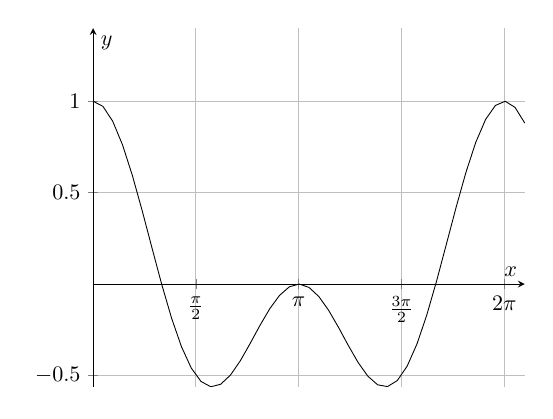
\begin{tikzpicture}[yscale=0.8, xscale=0.8]
			\begin{axis}[ 
				samples=45,
				xtick={-3.14159, -1.5708, 0,1.5708,3.14159,4.7123889, 6.28318},
				xticklabels={$-\pi$, $-\frac{\pi}{2}$, $0$,$\frac{\pi}{2}$,$\pi$,$\frac{3\pi}{2}$,$2\pi$},
				axis lines=middle,
				grid=major,
				ymax=1.4,
				xlabel=$x$,
				ylabel=$y$,
				]
				\addplot[domain=0:2.1*pi] {0.5*cos(deg(x)) + 0.5*cos(2*deg(x))} node[left]{};
			\end{axis}
		\end{tikzpicture}%
		\qquad
		\begin{tikzpicture}[yscale=0.8, xscale=0.8]
			\begin{axis}[
				axis lines=middle,
				xlabel=$k$,
				ylabel=$c_k$,
				ymin=0,
				ymax=1,
				%grid=major,
				xtick={0, 1, 2, 3, 4, 5, 6},
				xticklabels={0, 1, 2, 3, 4, 5, 6},
				enlargelimits,
				]
				\addplot[domain=0:6] {0} node[left]{};
				\tikzMegaFatLine{}{1,0}{1,0.5}
				\tikzMegaFatLine{}{2,0}{2,0.5}
			\end{axis}
		\end{tikzpicture}%
		\n \n
		$0.1 + 0.3 \cdot \cos(2x) + 0.6 \cdot \cos(6x)$: \\
%
		\noindent 
		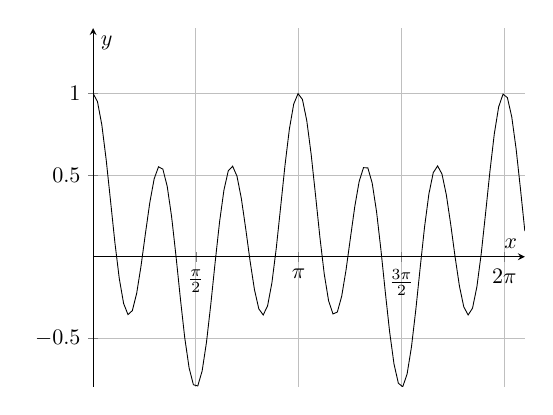
\begin{tikzpicture}[yscale=0.8, xscale=0.8]
			\begin{axis}[ 
				samples=100,
				xtick={-3.14159, -1.5708, 0,1.5708,3.14159,4.7123889, 6.28318},
				xticklabels={$-\pi$, $-\frac{\pi}{2}$, $0$,$\frac{\pi}{2}$,$\pi$,$\frac{3\pi}{2}$,$2\pi$},
				axis lines=middle,
				grid=major,
				ymax=1.4,
				xlabel=$x$,
				ylabel=$y$,
				]
				\addplot[domain=0:2.1*pi] {0.1 + 0.3*cos(2*deg(x)) + 0.6*cos(6*deg(x))} node[left]{};
			\end{axis}
		\end{tikzpicture}%
		\qquad
		\begin{tikzpicture}[yscale=0.8, xscale=0.8]
			\begin{axis}[
				axis lines=middle,
				xlabel=$k$,
				ylabel=$c_k$,
				ymin=0,
				ymax=1,
				%grid=major,
				xtick={0, 1, 2, 3, 4, 5, 6},
				xticklabels={0, 1, 2, 3, 4, 5, 6},
				enlargelimits,
				]
				\addplot[domain=0:6] {0} node[left]{};
				\tikzMegaFatLine{}{0,0}{0,0.1}
				\tikzMegaFatLine{}{2,0}{2,0.3}
				\tikzMegaFatLine{}{6,0}{6,0.6}
			\end{axis}
		\end{tikzpicture}%
	}
	
	\newpage
	\subsection{Diskrete Fourier-Transformation}
	
	\defi{
		\n 
		Die Idee hinter der Fourier-Transformation ist es, ein periodisches, diskretes Signal als Frequenzspektrum auszudrücken.
		Dies wird z.B. häufig im Zusammenhang mit Sound-Effekten ein "Muss".
		\n
		Die Eingabe einer Fourier-Transformation ist ein Vektor $v$, der aus Stützwerten (wie bei Interpolation) besteht. Diese Stützwerte sind immer äquidistant und im Intervall $[0, 2 \pi)$. Warum dieses Intervall? Naja, alle trigonometrischen Funktionen sind $2 \pi$ periodisch. Aus demselben Grund ist auch die obere Intervallgrenze $2\pi$ nicht mehr im Intervall, da es immer derselbe Wert sein muss wie bei $x=0$. Außerdem ähnlich zu Interpolation ist jetzt das Prinzip, das wir anwenden. Im Grunde machen wir einfache Interpolation mithilfe von Basisfunktionen (siehe \refChapter{chap:basisfunktionen}), nur mit trigonometrischen Basisfunktionen im komplexen Bereich, um 3D Signale abdecken zu können.
		\n
		Wenn man es implementiert, erkennt man, dass es sich lediglich um eine Vektor-Matrix Multiplikation handelt, sprich die Laufzeit entspricht $\bigO(n^2)$.
	}

	\sbreak
	\methode{
		\n 
		Die Eingabe für die Diskrete Fourier Transformation (DFT) ist ein Vektor $v$. \\
		Mit 
		\begin{align} 
			\omega = \exp \l(i \cdot \frac{2 \pi}{n} \r) 
 		\end{align}
		und mit $n$ als die Größe des Eingabevektors $v$ ergibt sich die Formel:
		\begin{align} 
 			\DFT(v) := c_k = \frac{1}{n} \cdot \sum_{j=0}^{n-1}v_j \cdot \compl{\omega}^{jk} 
 		\end{align}
		Die Formel für die Inverse Diskrete Fourier Transformation (IDFT):
		\begin{align} 
 			\IDFT(c) := v_j = \sum_{k=0}^{n-1}c_k \cdot \omega^{jk}
		\end{align}
		\n
		In Matrix-Vektor Schreibweise schön darstellbar:
		\begin{align}
			\nvector{
				c_0 \\ c_1 \\ \vdots \\ c_{n-1}
			}
			 = c = M_{\DFT, n} \cdot v = \frac{1}{n}
			\begin{bmatrix}
				1 & 1 & 1 & \dots & 1 \\
				1 & \compl{\omega}^1 & \compl{\omega}^2 & \dots & \compl{\omega}^{(n-1)}\\
				\vdots & \vdots & \vdots & \ddots & \vdots\\
				1 & \compl{\omega}^{n-1} & \compl{\omega}^{2 \cdot (n-1)} & \dots & \compl{\omega}^{(n-1)(n-1)}
			\end{bmatrix} \cdot 
			\nvector{
				v_0 \\ v_1 \\ \vdots \\ v_{n-1}
			}
		\end{align}
		Das Inverse: 
		\begin{align}
			\nvector{
				v_0 \\ v_1 \\ \vdots \\ v_{n-1}
			}
			 = v = M_{\IDFT, n} \cdot c = 
			\begin{bmatrix}
				1 & 1 & 1 & \dots & 1 \\
				1 & \omega^1 & \omega^2 & \dots & \omega^{(n-1)}\\
				\vdots & \vdots & \vdots & \ddots & \vdots\\
				1 & \omega^{n-1} & \omega^{2 \cdot (n-1)} & \dots & \omega^{(n-1)(n-1)}
			\end{bmatrix} \cdot 
			\nvector{
				c_0 \\ c_1 \\ \vdots \\ c_{n-1}
			}
		\end{align}
	}

	\sbreak
	\defi{
		\n 
%		Es gelten folgende Zusammenhänge (die ich nicht beweisen werde, schaut dafür in entsprechende Musterlösungen):
		Außerdem können wir aus unserem Omega (also die Grundfrequenz) noch ein paar Infos ableiten:
		\begin{align*}
			\omega &= \exp \l(i \cdot \frac{2 \pi}{n} \r) \\
				&= \cos \l(\frac{2 \pi}{n} \r) + i \cdot \sin \l(\frac{2 \pi}{n} \r) \\
			\compl{\omega} &= \cos \l(\frac{2 \pi}{n} \r) - i \cdot \sin \l(\frac{2 \pi}{n} \r) = \omega^{-1}
		\end{align*}
		Da es also eigentlich nur einer Kosinus Kurve (im Realteil) und einer Sinuskurve (im Imaginärteil) entspricht, können wir eine Symmetrie und Periodik ableiten:
		\begin{align} 
			\omega^{k \cdot (n -j)} &= \omega^{-kj} &&\text{(Symmetrie)} \\
			w^{k\cdot j} &= w^{k \cdot (n + j)} = w^{(k + n) \cdot j} &&\text{(Periodik)}
		\end{align}
		Daraus können wir uns zum Beispiel für $n=3$ herleiten:
		\begin{align*}
			\compl{\omega}^4 &= \omega^2 = \compl{\omega} \\
			\omega^4 &= \compl{\omega}^2 = \omega
		\end{align*}
	}

	\sbreak
	\bsp{
		\begin{align*} 
 			v = (0, -1, 1)\trans
 		\end{align*}
		\begin{align*}
			\DFT(v) &= \frac{1}{3} \cdot 
			\begin{bmatrix}
				1 & 1 & 1 \\
				1 & \compl{\omega}^1 & \compl{\omega}^2 \\
				1 & \compl{\omega}^2 & \compl{\omega}^4 
			\end{bmatrix} \cdot 
			\nvector{
				0 \\ -1 \\ 1
			} \\
			&= \frac{1}{3} \cdot 
			\nvector{
				0 \\
				-\compl{\omega}^1 + \compl{\omega}^2 \\
				- \compl{\omega}^2 + \compl{\omega}^4
			}
			 = \frac{1}{3} \cdot 
			\nvector{
				0 \\
				\omega - \compl{\omega}\\
				\compl{\omega} - \omega
			}
		\end{align*}
		Jetzt wenden wir die Euler-Formel an (siehe \refChapter{chap:komplexeZahlen}):
		\begin{align*}
			\DFT(v) = \frac{1}{3} \cdot 
			\begin{bmatrix}
				0 \\
				(\cos(\frac{2 \pi}{3}) + i \cdot \sin(\frac{2 \pi}{3})) - (\cos(\frac{2 \pi}{3}) - i \cdot \sin(\frac{2 \pi}{3}))\\
				(\cos(\frac{2 \pi}{3}) - i \cdot \sin(\frac{2 \pi}{3})) - (\cos(\frac{2 \pi}{3}) + i \cdot \sin(\frac{2 \pi}{3}))
			\end{bmatrix}
		\end{align*}
		Mit 
		\begin{align*}
			\cos\l(\frac{2 \pi}{3}\r) = -0.5 \aae \sin\l(\frac{2 \pi}{3}\r) = \frac{\sqrt{3}}{2}
		\end{align*}
		\begin{align*}
			\DFT(v) &= 
			\nvector{
				0 \\
				(-0.5 + i \cdot \frac{\sqrt{3}}{6}) - (-0.5 - i \cdot \frac{\sqrt{3}}{6}) \\
				(-0.5 - i \cdot \frac{\sqrt{3}}{6}) - (-0.5 + i \cdot \frac{\sqrt{3}}{6})
			} \\
			&= 
			\nvector{
				0 \\
				(0 + i \cdot \frac{2\sqrt{3}}{6})\\
				(0 - i \cdot \frac{2\sqrt{3}}{6})
			}
		\end{align*}
	}


	\newpage
	\subsection{Schnelle (Inverse) Fourier-Transformation}
	
	\defi{
		\n 
		Die Fourier-Transformation lässt sich schneller implementieren.
		Die Idee hinter dieser schnellen Variante ist es, mithilfe des sogenannten "Butterfly-Operators" die Menge an redundanten Operationen durch Rekursion zu verkleinern. Dafür sortiert man in der sogenannten "Sortier-Phase" den Eingabevektor nach den Einträgen mit gerade und ungeraden Indizes rekursiv. Danach wendet man oben genannten Operator in der "Kombinationsphase" an und geht dabei die Rekursion Ebenen wieder nach oben.\\
		Es wird sogar deutlich schneller, die neue Laufzeit von IFFT (= Inverse Fast Fourier Transformation) liegt in $\bigO(n \cdot \log(n))$. \\
		Wir nutzen dafür die zwei Eigenschaften von Omega:
		\begin{align*} 
 			\omega^{k \cdot (n -j)} &= \omega^{-kj} &&\text{(Symmetrie)} \\
 			w^{k\cdot j} &= w^{k \cdot (n + j)} = w^{(k + n) \cdot j} &&\text{(Periodik)}
 		\end{align*}
	}

	\sbreak
	\methode{ Butterfly-Operator
		\n 
		Zwei Einträge eines Vektors $a_j$ und $b_j$ mit demselben Index $j$ werden immer zusammen mit dem Butterfly-Operator verbunden. Mit $\BFO$ als Butterfly-Operator ist definiert:
		\begin{align}
			\BFO(a_j, b_j) := (a_j + w^j \cdot b_j, a_j - w^j \cdot b_j)
		\end{align}
		Das Ergebnis sind die Einträge der neuen Vektoren.
		%
	}
		\picC{bfo.png}{0.35}{Der $\BFO$ schöner dargestellt. Links von dem Kreis ist die Eingabe (wobei streng genommen das $w^j$ auch eine Eingabe ist und rechts jeweils die Ausgaben, die jeweils die Vektor-Einträge der Eingabe überschreiben.}

	\newpage
	
	\bsp{\n
		Gegeben seien zwei Arrays mit jeweils einem Eintrag:
		\begin{align*}
			a_0 = 3 \qquad b_0 = 5
		\end{align*}
		Nun wenden wir den Butterfly-Operator an. Wir merken uns, dass unser Index $j = 0$ ist.
		\n
		Unser Ergebnis ist dann ein zweidimensionaler Vektor $z$ mit:
		\begin{align*}
			z &= \nvector{a_0 + w^0 \cdot b_0 \\ a_0 - w^0 \cdot b_0} \\
				&= \nvector{3 + 1 \cdot 5 \\ 3 - 1 \cdot 5} \\
				&= \nvector{8 \\ -2}
		\end{align*}
	}
	
	\picC{fft.jpg}{0.9}{Typische Skizze einer Fast Fourier Transformation mit 8 Einträgen.}
	
	\defi{
		\n 
		Obiges Bild zeigt die Kombinationsphase, in der die einzelnen Buckets mithilfe des $\BFO$ miteinander kombiniert werden. Links unten von jedem Eintrag steht dabei der Index, den der Eintrag in seinem Bucket hat. Das sind nämlich genau die $j$ Werte beim Kombinieren, wie die Einträge neben den $\BFO$ Strichen zeigt (also dieses Kreuz mit dem Kreis entspricht dem $\BFO$).
		\n 
		Dass die Einträge in jedem Schritt anders benannt wurden, spielt nicht wirklich eine Rolle und soll nur zeigen, dass sich die Werte ändern, nicht aber die Positionen. 
		\n
		Wichtig: $\omega$ ist weiterhin $\exp\l(\frac{2\pi i}{n} \r)$, aber $n$ ist bei jedem Kombinationsschritt anders! So ist $n=2$ bei dem ersten Kombinationsschritt, $n=4$ bei dem danach und so weiter\dots
		\n 
		Auf dem Musterlösungsblatt kann man auch ein rasches Codebeispiel für $\FFT$ von der Übungsleitung finden.
 	}
	%
%	An dieser Stelle ein rasches Codebeispiel für FFT (Pseudo-Code):
%	FUNCTION [v[0], ..., v[n-1]] = IFFT(c[0], ..., c[n-1], n)
%		if n == 1:
%			v[0] = c[0];
%		else:
%			m = n / 2;
%			z1 = IFFT(c[0], c[2], ..., c[n-2], n/2);
%			z2 = IFFT(c[1], c[3], ..., c[n-1], n/2);
%			omega = exp(2 * pi * i / n);
%			for j = 0, ..., m-1:
%				v[j] = z1[j] + omega^j * z2[j];
%				v[m+j] = z1[j] - omega^j * z2[j];
%			end
%		end
%		return v;
                    % Fourier + FFT

% ---------------------------------------------------------------------------
% Quadratur
% ---------------------------------------------------------------------------
	
	\newpage
% =========================================================
	\section{Quadratur}
% =========================================================

	\defi{
		\n 
		Nachdem wir herausgefunden haben, wie wir eine Funktion mithilfe von Interpolation annähern können, drängt sich sofort die Frage auf, wie das mit der Integration einer Funktion aussieht.
		\n
		Es geht nicht nur, sondern auch noch recht simpel. Wir interpolieren die Funktion mithilfe von schon besprochenen Methoden und integrieren dann einfach analytisch. So integrieren wir eine Annäherung der Funktion und erhalten damit auch eine Approximation des Integrals. Dies ist die Kategorie der Quadratur-Probleme.
	}

	\sbreak
	\methode{ \label{sec:quadratur_regeln}
		\n 
		Allgemeines Quadraturproblem: 
		\begin{align*} 
 			\int_{a}^{b}f(x)\d x \approx \sum_{i=1}^{n}f(x_i) \cdot w_i 
 		\end{align*}
 		Die $w_i$ nennt man Gewichtungen, also wir gewichten $f(x_i)$ Werte, die ja den Stützwerten entsprechen. Aus der Kombination an Stützwerten und deren Gewichtungen erhalten wir eine approximative Lösung.
 		\n
		Sehr einfach mit Lagrange (siehe \refChapter{sec:lagrange_basis}):
		\begin{align*} 
 			f(x) &\approx p(x) = \sum_{i=1}^{n}f(x_i)\cdot L_i(x) \\
 			\longrightarrow \int_{a}^{b}f(x)\d x &\approx \int_{a}^{b}p(x) \d x = \int_{a}^{b}\sum_{i=1}^{n}f(x_i)\cdot L_i(x) \d x
		\end{align*}
		Für 2 Stützpunkte erhalten wir die Formel: 
		\begin{align} 
 			\QT(f) = H \cdot \frac{1}{2}\cdot \l(f(a) + f(b)\r)
 		\end{align}
		Wir nennen diese Formel die \fat{Trapezregel}.
		\n 
		Für 3 Stützpunkte erhalten wir die Formel: 
		\begin{align} 
 			\QS(f) = H \cdot \frac{1}{6} \cdot \l( f(a) + 4\cdot f\l(\frac{a+b}{2}\r) + f(b) \r) \label{eq:simpsonregel}
 		\end{align} 
		Diese Formel nennt man die \fat{Simpsonregel} (oder nach Johannes Kepler gibt es das Synonym \fat{Keplersche Fassregel}) und ist genauer als die Trapezregel.
		\n 
		Die Variable $H$ entspricht hierbei der Länge des zu integrierenden Bereichs, also $H = b-a$.
%	}
	%
		\begin{figure}[H]
			\centering
				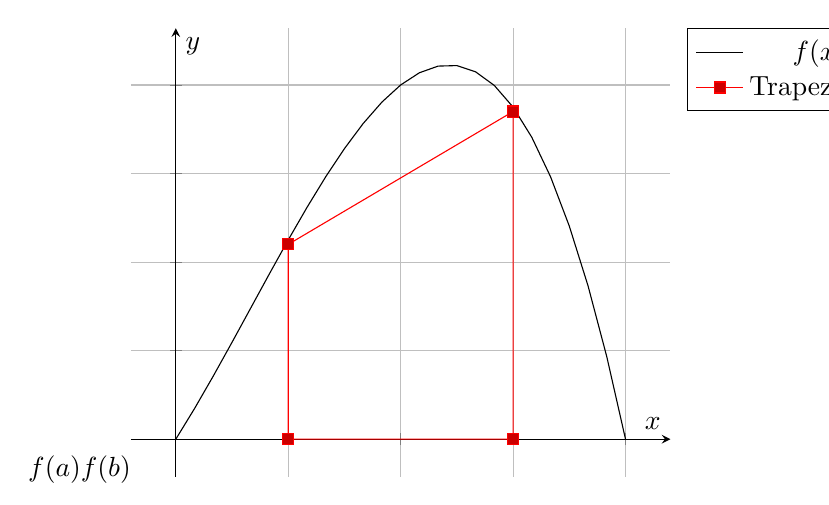
\begin{tikzpicture}
					\begin{axis}[
						axis lines=middle,
						xlabel=$x$,
						ylabel=$y$,
						enlargelimits,
						grid=major,
						xticklabels={,,},
						yticklabels={,,},
						%ymax=2,
						%ymin=-0.5,
						legend pos=outer north east,
						]
						\addplot[domain=0:2] {-1*x^3 + x^2 + 2*x} node[left]{};
						\addplot coordinates {
							( 0.5, 1.1 )
							( 1.5, 1.85 )
							( 1.5, 0)
							( 0.5, 0)
							( 0.5, 1.1)
						};
						\tikzPointLeft{$f(a)$}{0.5,1.1}
						\tikzPointRight{$f(b)$}{1.5,1.85}
						\legend{$f(x)$,Trapezregel}
					\end{axis}
				\end{tikzpicture}
			\caption{Ein zufälliges Beispiel einer Trapezregel. $a$ und $b$ jeweils wie in der Formel rechnet die Trapezregel die umrandete Fläche aus.}
		\end{figure}
	}

	\sbreak
	\bsp{
		\n
		Wir möchten $\int_{1}^{2}f(x) \d x$ einer Funktion $f(x)$ ausrechnen, bei denen wir nur die Stützpunkte $s_0: f(1) = 2$ und $s_1: f(2) = 4$ kennen.
		\\
		Nach der Trapezregel ergibt sich also: 
		\begin{align*} 
 			\QT(f) = 1 \cdot \frac{1}{2} \cdot (2 + 4) = 3 
 		\end{align*}
	}

	\sbreak
	\bsp{
		\n 
		Wir haben die Funktion $f(x) = \sin(x)$. Wir sollen mit den Stellen $x_0 = 0$ und $x_1=\pi$ und der Trapezregel die Fläche in diesen Bereich annähern.
		\begin{align*} 
			\QT(f) &= \pi \cdot 0.5 \cdot (f(0) + f(\pi))\\
				&= \pi \cdot 0.5 \cdot (\sin(0) + \sin(\pi))\\
				&= \pi \cdot 0.5 \cdot (0) \\
				&= 0
		\end{align*}
		Die Trapezregel schätzt, dass die Fläche $0$ ist. Wir wissen aber, dass der Sinus zwischen $0$ und $\pi$ eine Fläche deutlich größer $0$ hat.
		\newpage
		\begin{figure}[H]
			\centering
				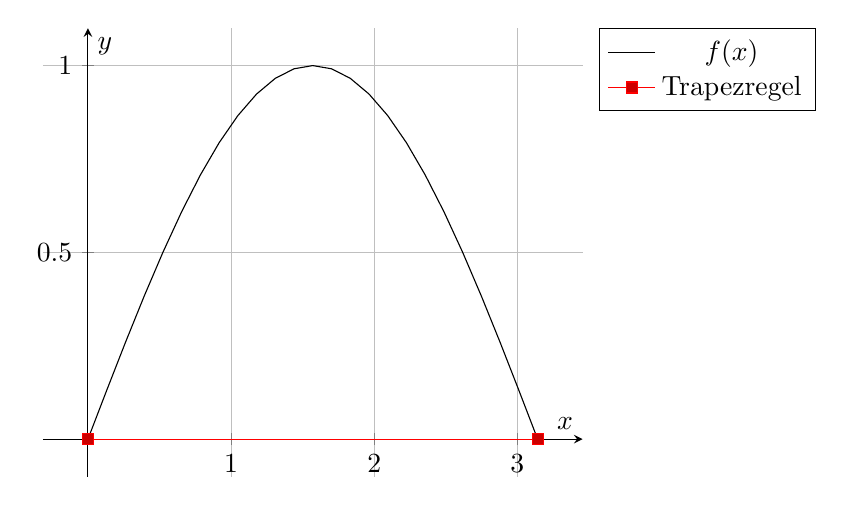
\begin{tikzpicture}
					\begin{axis}[
						axis lines=middle,
						xlabel=$x$,
						ylabel=$y$,
						enlargelimits,
						grid=major,
						ytick={0,0.5,1},
						legend pos=outer north east,
						]
						\addplot[domain=0:pi] {sin(deg(x))} node[left]{};
						\addplot coordinates {
							( 0, 0 )
							( pi, 0 )
						};
						\legend{$f(x)$,Trapezregel}
					\end{axis}
				\end{tikzpicture}
			\caption{Das Problem grafisch. Die Fläche unter dieser Sinuskurve ist definitiv nicht $0$!}
			\label{fig:sinus0}
		\end{figure}
		\noindent Hieran kann man sehen, dass es Fälle gibt, wo die Abschätzung schlecht bis sehr schlecht sein kann.
	}

	\lbreak
	\wichtig{
		\n
		Wir können mit einem Interpolationspolynom vom Grad $2 \cdot n$ ein Polynom vom Grad $2\cdot n+1$ noch exakt integrieren. (ein gerader Grad integriert den nächst höheren ungeraden Grad noch exakt)
	}

	\sbreak
	\bsp{
		\n
		Eine Konstante (Grad 0) kann eine Gerade (Grad 1) exakt integrieren\\
		Aber eine Gerade (Grad 1) kann keine Parabel (Grad 2) exakt integrieren.
	}

	\newpage
	\defi{ \label{defi:quadratur_kondition}
		\n
		Warum erstellt man nicht eine "Regel" mit sehr viel mehr Stützpunkten? 
		\n 
		Das Problem hierbei ist die Kondition. Die entspricht nämlich der Summe aller Beträge der Gewichtungen $\omega$.
		\begin{align} 
 			\sum_i |\omega_i| 
 		\end{align}
		In aller Regel sind die Gewichtungen positiv und ergeben aufaddiert immer 1. Bei Trapezregel ist es $0.5 + 0.5 = 1$, bei Simpsonregel $\nicefrac{1}{6} \cdot (1 + 4 + 1) = 1$ und so weiter.
		Bei deutlich mehr Stützpunkten pro "Regel" (etwa ab 8) werden manche Gewichtungen negativ und somit die Summe der Beträge nicht mehr eins und damit schlechter.
		\n 
		Wir probieren das Problem der Ungenauigkeit auf andere Weise zu verringern. Das behandeln wir im nächsten Kapitel.
	}

	\newpage
	\subsection{Klassische Quadratur}
	\defi{
		\n
		Komplizierte Funktionen liefern meist schlechte Ergebnisse. Die Idee diese zu lösen ist denkbar einfach: Wir wenden die Quadraturregeln stückweise an und unterteilen unser Problem in viele Teilprobleme.
	}

	\sbreak
	\methode{
		\n 
		Beschreibt $H$ den zu integrierenden Bereich (also zwischen $a$ und $b$), $h$ die Länge der einzelnen Stücke, in der wir das Problem aufteilen und $N$ die Anzahl jener. \n
		Formell: 
		\begin{align*} 
 			H &= b - a \aae h = \frac{b-a}{N} \\
			f_i &= f(x_i) \aae x_i = a + i\cdot h 
 		\end{align*}
		\begin{align*} 
 			\QT(f) = H \cdot \frac{f(a) + f(b)}{2} 
 		\end{align*}
		\begin{align} 
 			\rightarrow \QTS(f;h) = h \cdot \l(\frac{f_0}{2} + f_1 + \dots + f_{N-1} + \frac{f_N}{2} \r)
 		\end{align}
		$\QTS$ entspricht dann der \fat{Trapezsumme}.
		\begin{align*} 
			\QS(f) = H \cdot \frac{f(a) + 4 \cdot f\l(\frac{a + b}{2}\r) + f(b)}{6} 
 		\end{align*}
		\begin{align} 
 			\rightarrow \QSS(f;h) = \frac{h}{3}\cdot \l(f_0 + 4f_1 + 2f_2 + 4f_3 + \dots + 2f_{N-2} + 4f_{N-1} + f_N \r)
		\end{align}
		$\QSS$ nennt man die \fat{Simpsonsumme}. Benannt ist dies nach Thomas Simpson.
	}

	\newpage
	\bsp{
		\begin{figure}[H]
			\centering
				\begin{tikzpicture}
					\begin{axis}[
						axis lines=middle,
						xlabel=$x$,
						ylabel=$y$,
						enlargelimits,
						%xticklabels={,,},
						%yticklabels={,,},
						ymax=3.1,
						%ymin=-0.5,
						legend pos=outer north east,
						]
						\addplot[domain=0:2.5] {-1*x^3 + x^2 + 2*x} node[left]{};
						\addplot[dash pattern=on 1pt off 3pt on 3pt off 3pt] coordinates {
							(0.5, 1.1)
							(1, 2)
							(1.5, 1.85)
							(2, 0)
							(2.5, -4.35)
							(2.5, 0)
							(2, 0)
							(1.5, 0)
							(1.5, 1.85)
							(1.5, 0)
							(1, 0)
							(1, 2)
							(1, 0)
							(0.5, 0)
							(0.5, 1.1)
						};
						\addplot[dotted] coordinates {
							(0.5, 0)
							(0.5, 1.1)
							(2.5, -4.35)
							(2.5, 0)
							(0.5, 0)
						};
						\tikzPointLeft{$f(a)$}{0.5,1.1}
						\tikzPointUp{$f(a) + h$}{1,2}
						\tikzPointLeft{$f(b)$}{2.5,-4.35}
						\legend{$f(x)$,Trapezsumme, Trapezregel}
					\end{axis}
				\end{tikzpicture}
			\caption{Beispiel einer Trapezsumme, bei der $N=4$ (in dieser Grafik die gestrichelte Linie) Trapeze konstruiert worden sind, um die Fläche besser anzunähern. Im Vergleich zeigt die gepunktete Linie die Annäherung durch die Trapezregel, also einem Trapez.}
		\end{figure}
	}

	\sbreak
	\bsp{
		\n 
		Und wenn wir uns auch noch einmal das Problem vorher mit Sinus anschauen (siehe \refFigure{fig:sinus0}) sehen wir, dass mehr Trapeze zu einer höheren Genauigkeit führt.
		\begin{figure}[H]
			\centering
				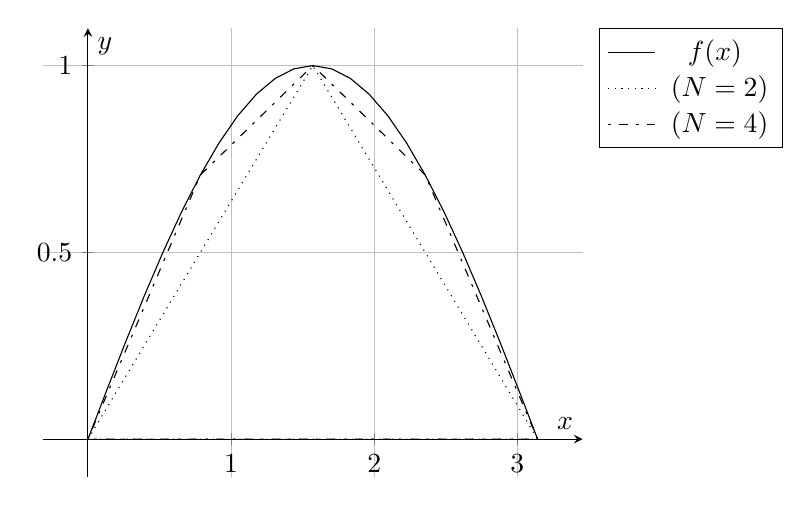
\begin{tikzpicture}
					\begin{axis}[
						axis lines=middle,
						xlabel=$x$,
						ylabel=$y$,
						enlargelimits,
						grid=major,
						ytick={0,0.5,1},
						legend pos=outer north east,
						]
						\addplot[domain=0:pi] {sin(deg(x))} node[left]{};
						\addplot[dotted] coordinates {
							( 0, 0 )
							( pi / 2, 1 )
							( pi, 0 )
							( 0, 0 )
						}; %0.70710678__1186547524400844362104849039284835937688474036588...
						\addplot[dash pattern=on 1pt off 3pt on 3pt off 3pt] coordinates {
							( 0, 0 )
							( pi / 4, 0.70710678 )
							( pi / 2, 1 )
							( (3 * pi) / 4, 0.70710678 )
							( pi, 0 )
							( 0, 0 )
						};
						\legend{$f(x)$, $\QTS$ ($N=2$), $\QTS$ ($N=4$)}
					\end{axis}
				\end{tikzpicture}
			\caption{Die Approximation ist definitiv besser geworden.}
		\end{figure}
	}

	\sbreak
	\subsection{Restglied}

	\defi{
		\n 
		Unter dem sogenannten "Restglied" z.B. einer Trapezsumme beschreibt man die Fehlerabschätzung. Im Grunde also $\RTS \approx \QTS - I(f)$. Diesen Fehler schätzt man nach folgender Formel ab: \n 
		Restglied $\RTS:$ 
		\begin{align} 
 			\RTS(f;h) = h^2 \cdot H \cdot \frac{f^{(2)}(\xi)}{12} 
 		\end{align}
 		Das ganze gibt es dann noch für die Simpsonsumme.
 		\begin{align} 
 			\RSS(f;h) = h^4 \cdot H \cdot \frac{f^{(4)}(\xi)}{180} 
 		\end{align}
 		Das $\xi$ kommt aus dem Mittelwertsatz. Man nimmt hierfür, wenn nötig, meist den Wert aus dem Intervall, dass die Fehlerabschätzung den maximalen Fehler abschätzt und damit den "worst-case".
 		\n 
 		Es ist ziemlich analog zur Fehlerabschätzung einer Polynom-Interpolation, siehe \refChapter{sec:interpolation_fehler}.
	}                  % Klassische Quadratur
	\newpage
	\subsection{Quadratur nach Romberg}
	
	\defi{
		\n 
		Quadratur nach Romberg kombiniert zwei Trapezsummen unterschiedlicher Schrittweiten, um das exakte Ergebnis besser zu approximieren. Wir können das iterativ mit jeweils zwei und insgesamt mehr als zwei Trapezsummen machen, um eine höhere Genauigkeit zu erhalten.
		\n
		Wir konstruieren uns dafür Trapezsummen mit immer kleinerem $h$ bzw. größerem $N$, die wir auch inkrementell bestimmen können. Es gilt nämlich:
		\begin{align}
			\QTS(f;h) = \frac{\QTS(f; 2h)}{2} + h \cdot \l(f_1 + f_3 + \dots + f_{N-3} + f_{N-1} \r)
		\end{align}
		Die Romberg-Quadratur ist im Grunde eine \fat{Extrapolation}. Mithilfe der Kombination von Trapezsummen schätzt die Romberg-Quadratur den Wert an der Stelle $h=0$ ab, was im Prinzip dem analytischen Ergebnis entsprechen sollte (schrittweite von 0 wäre ja theoretisch die perfekte Approximation).
		\begin{figure}[H]
			\centering
			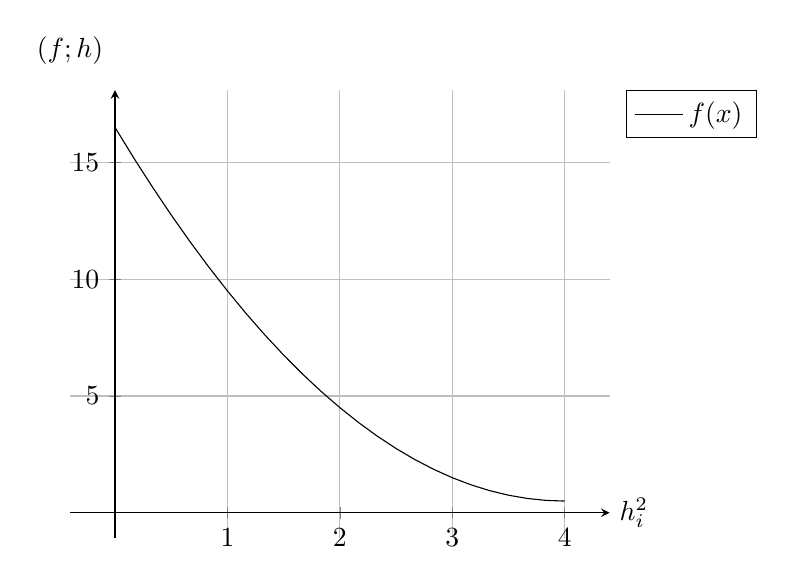
\begin{tikzpicture}
			\begin{axis}[
			axis lines=middle,
			xlabel=$h_i^2$,
			ylabel=$\QTS(f; h)$,
			enlargelimits,
			grid=major,
			%ytick={0,0.5,1},
			legend pos=outer north east,
			every axis x label/.style={at={(current axis.right of origin)},anchor=west},
			every axis y label/.style={at={(current axis.north west)},above=2mm},
			]
			\addplot[domain=0:4] {x^2 - 8*x + 16.5} node[left]{};
			\tikzPointUp{}{4,0.5}
			\tikzPointUR{}{2,4.5}
			\tikzPointUR{}{1,9.5}
			\tikzPointRight{}{0,16.5}
			\legend{$f(x)$}
			\end{axis}
			\end{tikzpicture}
			\caption{Die rechten drei Punkte sind hier die Werte von drei Trapezsummen. Durch diese kann der Punkt an der Stelle $h^2 = 0$ abgeschätzt werden. Das ist dann das Ergebnis der Romberg-Quadratur.}
		\end{figure}
	}

	\newpage
	\methode{\n
		Zum Kombinieren können wir ähnlich dem Newton und Aitken-Neville Verfahren eine Tabelle schreiben, die nach \fat{rechts unten} determiniert.
		\begin{table}[H]
			\label{table:romberg}
			\centering
			\begin{tabular}{cc|cccc}
				\toprule
				$h_k$  & $k$ & $Q_{k0}$ & $Q_{k1}$ & \dots & $Q_{kn}$ \\ \midrule
				$\frac{b-a}{1}$ & $0$ & $\QTS(f;\frac{b-a}{1}) = Q_{00}$ &  & & \\
				$\frac{b-a}{2}$ & $1$ & $\QTS(f;\frac{b-a}{2}) = Q_{10}$ & $Q_{11}$ &  & \\
				$\frac{b-a}{4}$ & $2$ & $\QTS(f;\frac{b-a}{4}) = Q_{20}$ & $Q_{21}$ & $Q_{22}$ & \\
				\vdots & & \vdots & & & $\ddots$ \\
			\end{tabular}
			\caption{Tabelle zum ausrechnen}
		\end{table}
		\noindent Mit folgender Gleichung kombinieren wir zwei beliebige Trapezsummen $\QTS(f, h_1)$ und $\QTS(f, h_2)$:
		\begin{align} 
 			\QTS(f, h_{\text{neu}}) = \QTS(f, h_2) + \frac{\QTS(f, h_2) - \QTS(f, h_1)}{\l(\frac{h_1^2}{h_2^2}\r) - 1} 
 		\end{align}	
		Informell und direkt auf das Dreiecksschema angepasst:
		\begin{align} 
 			Q_{\text{neu}} = Q\uleft + \frac{Q\uleft - Q\uleftUp}{\l(\frac{h\uleftUpDiagonal}{h\uleft}\r)^2 - 1} 
 		\end{align} 
 		Von der Notation her wie bei Newton-Verfahren (siehe \refChapter{chap:newtoninterpolation}), nur halt jetzt mit "links" statt "rechts" und anstelle von "unten" ist es halt darüber, also "oben".
	}

	\newpage
	\bsp{
		\n 
		% x^2 - 4
		Wir möchten folgende Berechnung annähern:
		\begin{align*} 
 			\int_{1}^{3}f(x) \d x
		\end{align*}
		Folgende Stützpunkte seien bekannt:
		\begin{table}[H]
			\label{table:ex_romberg}
			\centering
			\begin{tabular}{rccccc}
				\toprule
				$x$   	& $1$ 	& $1.5$ 	& $2$ 	& $2.5$		& $3$ \\ \midrule
				$f(x)$ 	& $-3$ 	& $-1.75$ 	& $0$   & $2.25$ 	& $5$    \\
				\bottomrule
			\end{tabular}
		\end{table}
		Damit können wir Romberg-Quadratur bis zu drei Trapezsummen aufstellen:
		\begin{table}[H]
			\label{table:ex_romberg_table}
			\centering
			\begin{tabular}{cc|ccc}
				\toprule
				$h_k$  & $k$ & $Q_{k0}$ & $Q_{k1}$ & $Q_{k2}$ \\ \midrule
				$\frac{b-a}{1}$ & $0$ & $\QTS(f;\frac{b-a}{1}) = Q_{00}$ &  & \\
				$\frac{b-a}{2}$ & $1$ & $\QTS(f;\frac{b-a}{2}) = Q_{10}$ & $Q_{11}$ &  \\
				$\frac{b-a}{4}$ & $2$ & $\QTS(f;\frac{b-a}{4}) = Q_{20}$ & $Q_{21}$ & $Q_{22}$
			\end{tabular}
		\end{table}
		\begin{align*} 
 			\QTS&(f;h) = h \cdot (\frac{f_0}{2} + f_1 + ... + f_{N-1} + \frac{f_N}{2}) \\
 			Q_{00} &= \QTS(f, \frac{b-a}{1}) = \QT(f) = 2 \cdot \frac{f(1) + f(3)}{2} = 2 \cdot \frac{-3 + 5}{2} = 2 \\
 			Q_{10} &= \QTS(f, \frac{b-a}{2}) = \QTS(f, 1) = 1 \cdot (\frac{-3}{2} + 0 + \frac{5}{2}) = 1 \\
			Q_{20} &= \QTS(f, \frac{b-a}{4}) = \QTS(f, 0.5) = 0.5 \cdot (\frac{-3}{2} - 1.75 + 0 + 2.25 + \frac{5}{2}) = 0.75 
 		\end{align*}
%		Tragen wir ein, was wir wissen:
%				$h_k$  & $k$ & $Q_{k0}$ & $Q_{k1}$ & $Q_{k2}$ \\ \midrule
%				$2$ & $0$ & $2$ &  & \\
%				$1$ & $1$ & $1$ & $Q_{11}$ &  \\
%				$0.5$ & $2$ & $0.75$ & $Q_{21}$ & $Q_{22}$ \\
		Jetzt geht es an das Kombinieren mit der Formel:
		\begin{align*} 
 			Q_{\text{neu}} &= Q\uleft + \frac{Q\uleft - Q\uleftUp}{\l(\frac{h\uleftUpDiagonal}{h\uleft}\r)^2 - 1}  \\
			Q_{11} &= 1 + \frac{1 - 2}{(\frac{2}{1})^2 - 1} = \frac{2}{3} \\
			Q_{21} &= 0.75 + \frac{0.75 - 1}{(\frac{1}{0.5})^2 - 1} = \frac{8}{12} 
 		\end{align*}
		\begin{table}[H]
			\label{table:ex_romberg_table3}
			\centering
			\begin{tabular}{cc|ccc}
				\toprule
				$h_k$  & $k$ & $Q_{k0}$ & $Q_{k1}$ & $Q_{k2}$ \\ \midrule
				$2$ & $0$ & $2$ &  & \\
				$1$ & $1$ & $1$ & $\nicefrac{2}{3}$ &  \\
				$0.5$ & $2$ & $0.75$ & $\nicefrac{8}{12}$ & $Q_{22}$ \\
			\end{tabular}
		\end{table}
		Jetzt noch das Ergebnis ausrechnen:
		\begin{align*} 
 			Q_{22} = \frac{8}{12} + \frac{\frac{8}{12} - \frac{2}{3}}{(\frac{2}{0.5})^2 - 1} = \frac{8}{12} + \frac{\frac{8}{12} - \frac{8}{12}}{16 - 1} = \frac{8}{12} = \frac{2}{3} 
 		\end{align*}
		In diesem Fall ist das Ergebnis schon exakt, da die unbekannte Funktion $f$ in Wahrheit $f(x) = x^2 - 4$ ist und die Fläche von $1$ bis $3$ analytisch exakt $\frac{2}{3}$ entspricht.
		\begin{figure}[H]
			\centering
			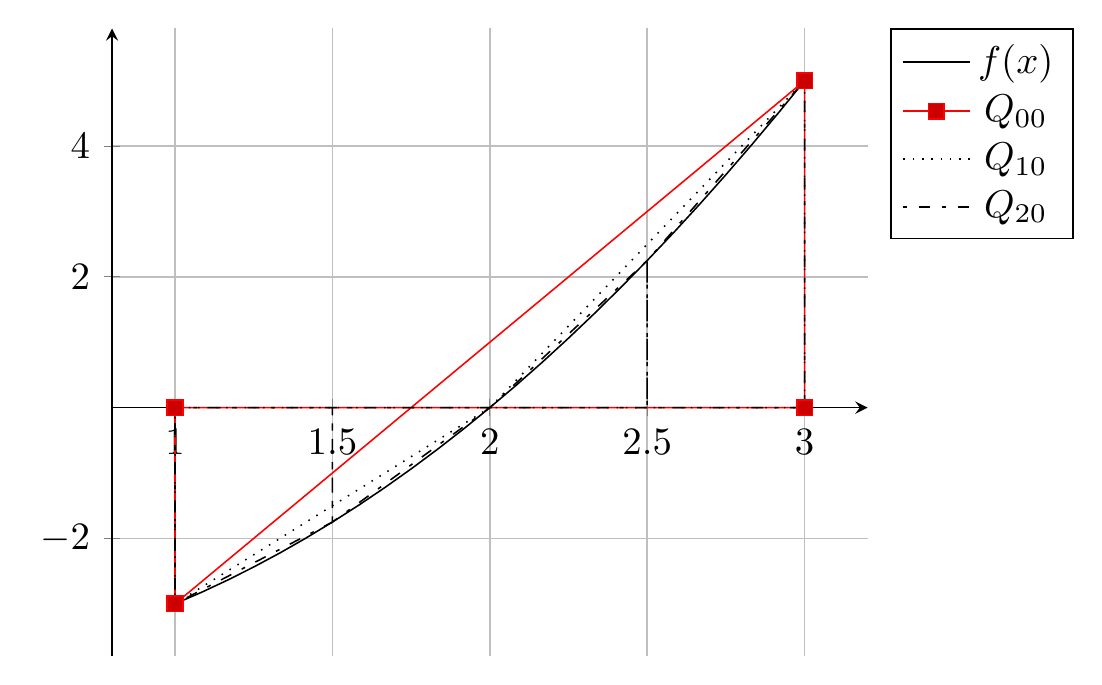
\begin{tikzpicture}[scale=1.4]
				\begin{axis}[
					axis lines=middle,
					xlabel=,
					ylabel=,
					enlargelimits,
					grid=major,
					%ymax=3.1,
					%ymin=-0.5,
					legend pos=outer north east,
					]
					\addplot[domain=1:3] {x^2 - 4} node[left]{};
					\addplot coordinates {
						(1, 0)
						(1, -3)
						(3, 5)
						(3, 0)
						(1, 0)
					};
					\addplot[dotted] coordinates {
						(1, 0)
						(1, -3)
						(2, 0)
						(3, 5)
						(3, 0)
						(1, 0)
					};
					\addplot[dash pattern=on 1pt off 3pt on 3pt off 3pt] coordinates {
						(1, 0)
						(1, -3)
						(1.5, -1.75)
						(1.5, 0)
						(1.5, -1.75)
						(2, 0)
						(2.5, 2.25)
						(2.5, 0)
						(2.5, 2.25)
						(3, 5)
						(3, 0)
						(1, 0)
					};
					\legend{$f(x)$,$Q_{00}$, $Q_{10}$, $Q_{20}$}
				\end{axis}
			\end{tikzpicture}
			\caption{Die verschiedenen Trapezsummen, die wir in dem Beispiel genutzt haben sowie die exakte Funktion.}
		\end{figure}
	}          % Romberg
	\newpage
	% -----------------------------------------
	\subsection{Gauß Quadratur}
	
	\defi{
		\n 
		Bisher haben wir bei der Interpolation mit den verschiedenen Methoden hauptsächlich die sogenannte Gewichtung einzelner Stützstellen ausgerechnet. Z.B. hatte die Trapezregel (siehe \refChapter{sec:quadratur_regeln}) eine Gewichtung von $0.5$ bei beiden Stützstellen.
		\n 
		Die Gauß Quadratur gibt jetzt nicht nur die Gewichtung der einzelnen Stützstellen, sondern auch die Position der Stützstellen selbst vor, um die Anzahl der Bedingungen zu verdoppeln. Der erreichbare Polynomgrad liegt also bei $(2\cdot n - 1)$ bei $n$ Stützstellen, was ziemlich hoch ist.
		\n 
		Eine Einschränkung ist, dass das Integrationsgebiet immer von $-1$ bis $1$ geht. Andere Intervalle müssen wir also ähnlich wie bei Hermite-Interpolation (siehe \refChapter{chap:hermite_interpolation}) erst einmal strecken und verschieben bzw. transformieren, also ist diese Einschränkung eigentlich kein Thema.
		\n 
		Außerdem erhalten wir bei der Gauß-Quadratur nur positive Gewichte $w_i$, wodurch die Quadraturformel immer stabil bleibt, die Kondition immer gleich $b-a$ ist (siehe \refChapter{defi:quadratur_kondition}). Um eine Gauß-Quadratur Formel herzuleiten, wird die "Methode der unbestimmten Koeffizienten" verwendent.
	}
	
	\sbreak
	\methode{ Methode der unbestimmten Koeffizienten:
		\n 
		Wir können folgende Gleichung aufstellen, die im Grunde unser allgemeines Quadraturproblem zusammenfasst. Nämlich die Summe von Funktionswerten mal Gewichtungen soll gleich dem Integralwert der Funktion entsprechen.
		\begin{align} 
 			\sum_{i=0}^{n}f(x_i)\cdot w_i \shouldEq \int_{a}^{b}f(x) \d x 
 		\end{align}
 		Diesen Term kann man nun für unterschiedliche Grade aufschreiben, wo diese gelten sollen (bei $n$ Stützstellen darf ja nach Gauß-Quadratur der bis zum $(2 \cdot n - 1)$'ten Grad erreicht werden). Danach versuchen wir, dass alle aufgestellten Gleichungen erfüllt werden (ähnlich zu einem LGS). Damit kann man dann auf alle $x_i$ und alle $w_i$ schließen und damit die Regel der entsprechenden Gauß-Quadratur.
 		\n
 		Die Funktion $f(x)$ entspricht natürlich den Standard Polynom Grad Funktionen, also für Grad 0 wäre $f(x) = 1$, für Grad 1 ist es $f(x) = x$ usw.
	}
	
	\newpage
	\bsp {
		\n 
		Es soll eine unbekannte Funktion mithilfe von einer Stützstelle $x_0$ und der Gauß-Quadratur bestimmt werden. Mit einer Stützelle, also $n=1$, müssen wir die Grade von $0$ bis $(2 \cdot n) - 1 = 1$ aufstellen. \\
		Alle Informationen mithilfe von der obigen Formel aufschreiben: \n 
		Grad 0 mit $f(x) = 1$:
		\begin{align*}
			f(x_0) \cdot w_0 = w_0 \shouldEq \int_{-1}^{1}f(x)\d x = 2 
		\end{align*}
		Grad 1 mit $f(x) = x$:
		\begin{align*} 
			f(x_0) \cdot w_0 = w_0 x_0 \shouldEq \int_{-1}^{1}f(x)\d x = 0 
		\end{align*}
		Daraus können wir also folgern:
		\begin{align*}
			w_0 &= 2 \\
			w_0 x_0 &= 0 \\
			\Longrightarrow x_0 &= 0
		\end{align*}
		Das ist natürlich ein etwas bescheuertes Beispiel, da man mit einer Stützstelle niemals Gauß-Quadratur machen würde. Trotzdem interessant, dass man im Falle einer Stützstelle im besten Falle die in der Mitte des Bereiches nehmen sollte.
		\n
		\noindent Jetzt gibt es noch ein komplexeres Beispiel.
	}
	
	\sbreak
	\bsp{ 
		\n
		Gauß-Quadratur mit 3 Stützstellen an den Stellen $x_0 = -1 \aae x_1 = 0 \aae x_2 = 1$.
		Alle Informationen mithilfe von der obigen Formel aufschreiben: \n 
		Grad 0 mit $f(x) = 1$: 
		\begin{align*} 
			f(x_0) \cdot w_0 + f(x_1) \cdot w_1 + f(x_2) \cdot w_2 = w_0 + w_1 + w_2\shouldEq \int_{-1}^{1}f(x)\d x = 2 
		\end{align*}
		Grad 1 mit $f(x) = x$:
		\begin{align*} 
			f(x_0) \cdot w_0 + f(x_1) \cdot w_1 + f(x_2) \cdot w_2 = w_0x_0 + w_1x_1 + w_2x_2 \shouldEq \int_{-1}^{1}f(x)\d x = 0 
		\end{align*}
		Grad 2 mit $f(x) = x^2$:
		\begin{align*} 
			f(x_0) \cdot w_0 + f(x_1) \cdot w_1 + f(x_2) \cdot w_2 = w_0x_0^2 + w_1x_1^2 + w_2x_2^2 \shouldEq \int_{-1}^{1}f(x)\d x = \frac{2}{3}
		\end{align*}
		\n 
		Weil wir oben schon die Positionen der Stützstellen (vereinfachtes Beispiel) gegeben haben, müssen wir die Gleichung noch höherer Grade (wir könnten bis Grad 5 aufschreiben) nicht mehr verwenden, weil das genügend Informationen sind (noch drei Unbekannte, drei Gleichungen).
		\begin{align*}
			w_0 + w_1 + w_2 &= 2 &&(I)\\
			-w_0 + w_1 0 + w_2 &= 0 &&(II)\\
			w_0 + w_1 0 + w_2 &= \frac{2}{3} &&(III) \\
			\\
			\text{Wir können schließen:}& \\
			-w_0 + w_2 &= 0 &&(II)\\
			w_0 &= w_2 \\
			\\
			w_0 + w_2 &= \frac{2}{3} &&(III)\\
			w_0 &= \frac{2}{3} - w_2 \\
			\text{Einsetzen in (II):}& \\
			-\frac{2}{3} + w_2 + w_2 &= 0 \\
			2w_2 &= \frac{2}{3} \\
			w_2 &= w_0 = \frac{1}{3}\\
			\\
			\text{Den Rest erschließen:}&\\
			w_0 + w_1 + w_2 &= 2 &&(I)\\
			w_1 &= 2 - w_0 - w_2 = 2 - 2w_2 \\
			w_1 &= 2 - \frac{2}{3} = \frac{4}{3}
		\end{align*}
		Also zusammenfassend könnte man sagen, dass die Fläche einer unbekannten Funktion mit Gauß-Quadratur mit Stützstellen $-1, 0$ und $1$ folgendermaßen ausrechnet:
		\begin{align*}
			Q = f(-1) \cdot \frac{1}{3} + f(0) \cdot \frac{4}{3} + f(1) \cdot \frac{1}{3}
		\end{align*}
		Das könnte bekannt vorkommen, da das einfach \fat{Simpsonregel} (siehe \refEquation{eq:simpsonregel}) für unser spezifisches Beispiel ist \Winkey. \\
		Es ist äquivalent zu:
		\begin{align*}
			Q_S = 2 \cdot \frac{1}{6} \cdot \l(f(-1) + 4 f(0) + f(1) \r)
		\end{align*}
	}

	%-------------------------
	% ALTE BEISPIELE, DIE NOCH VERVOLLSTÄNDIGT WERDEN MÜSSEN
	
	%		Gauß-Quadratur mit 3 beliebigen Stützstellen $x_0, x_1, x_2$. Dadurch hat man auch drei Gewichtungen $w_0, w_1, w_2$. \\
	%		Alle Informationen mithilfe von der obigen Formel aufschreiben: \n 
	%		Grad 0 mit $f(x) = 1$: 
	%			f(x_0) \cdot w_0 + f(x_1) \cdot w_1 + f(x_2) \cdot w_2 = w_0 + w_1 + w_2\shouldEq \int_{-1}^{1}f(x)\d x = 2 
	%		Grad 1 mit $f(x) = x$:
	%			f(x_0) \cdot w_0 + f(x_1) \cdot w_1 + f(x_2) \cdot w_2 = w_0x_0 + w_1x_1 + w_2x_2 \shouldEq \int_{-1}^{1}f(x)\d x = 0 
	%		Grad 2 mit $f(x) = x^2$:
	%			f(x_0) \cdot w_0 + f(x_1) \cdot w_1 + f(x_2) \cdot w_2 = w_0x_0^2 + w_1x_1^2 + w_2x_2^2 \shouldEq \int_{-1}^{1}f(x)\d x = \frac{2}{3}
	%%		Grad 3 mit $f(x) = x^3$:
	%%			f(x_0) \cdot w_0 + f(x_1) \cdot w_1 + f(x_2) \cdot w_2 = w_0x_0^3 + w_1x_1^3 + w_2x_2^3 \shouldEq \int_{-1}^{1}f(x)\d x = 0
	%%		Grad 4 mit $f(x) = x^4$:
	%%			w_0x_0^4 + w_1x_1^4 + w_2x_2^4 \shouldEq \int_{-1}^{1}f(x)\d x = \frac{2}{5}
	%%		Grad 5 mit $f(x) = x^5$:
	%%			w_0x_0^5 + w_1x_1^5 + w_2x_2^5 \shouldEq \int_{-1}^{1}f(x)\d x = 0
	%		Um das Beispiel etwas zu vereinfachen gehen wir davon aus, dass $x_1 = 0$ sowie $x_0 = -x_2$ gilt. Aus diesem Grund müssen wir die Gleichung höherer Grades nicht mehr aufschreiben, weil das genügend Informationen sind.
	%			x_1 &= 0 \\
	%			x_0 &= -x_2 \\
	%			w_0 + w_1 + w_2 &= 2 \\
	%			w_0 x_0 + w_1 x_1 + w_2 x_2 &= 0 \\
	%			w_0 x_0^2 + w_1 x_1^2 + w_2 x_2^2 &= \frac{2}{3}
	%		Jetzt können wir das auflösen: (2. Gleichung)
	%			w_0 x_0 + w_1 0 + w_2 x_2 &= 0 \\
	%			w_0 x_0 + w_2 x_2 &= 0 \\
	%			w_0 x_0 &= -w_2 x_2 \\
	%			w_0 x_0 &= w_2 x_0 \\
	%			w_0 &= w_2
	%%		Da $x_0 = x_2 = 0$ nicht sein kann, können wir außerdem schließen: (2. Gleichung)
	%%			w_0x_0 + w_1x_1 &= 0
	%		Und damit: (1. Gleichung)
	%			w_0 + w_1 + w_2 &= 2 \\
	%			2 - w_1 &= 2w_0 = 2w_2 \\
	%		Dritte Gleichung:
	%			w_0w_0 x_0^2 + w_1 x_1^2 + w_2 x_2^2 &= \frac{2}{3} \\
	%			w_0 x_0^2 + w_2 x_2^2 &= \frac{2}{3} \\
	%			2w_0x_0^2 &= \frac{2}{3}
	
	%		Wenn man dies nun weiterführt, kommt man auf folgende Ergebnisse (davon ausgehend, dass $x_0 = -x_1$)
	%			w_0 = w_1 = 1 \aae x_0 = \frac{1}{\sqrt{3}} \aae x_1 = -\frac{1}{\sqrt{3}} 
	%		Um nun also auf das Integral zu schließen, muss man nur noch den Stützwert an der Stelle $x_0$ und $x_1$ ausrechnen, mit ihrer Gewichtung multiplizieren und dann schlussendlich addieren. \\
	%Mit mehr Stützstellen geht das dann natürlich analog.

	\sbreak
	\defi{
		\n 
		Sobald wir alle $x_i$ und $w_i$ aufgestellt haben, können wir die entstandene Formel nutzen, um das Integral einer Funktion anzunähern.
		\n 
		Das geht dann wie gewohnt mit folgender Formel:
		\begin{align}
			\sum_{i=0}^{n-1}f(x_i)\cdot w_i
		\end{align}
		Die $f(x_i)$ müssen wir unter Umständen noch ausrechnen. In der Praxis ist das deswegen insofern relevant, weil die Gauß-Quadratur im Grunde über \fat{Gewichtung und Stützposition} optimiert. 
		\n 
		Sprich wenn ein Stützwert auszurechnen kostenaufwändig ist (weil man die Funktion zwar gegeben hat, diese aber sehr komplex ist auszuwerten), dann könnte man zu einer bestimmten Anzahl beliebig zu wählender Stützstellen die Quadratur mit Gauß optimieren.
		\n 
		Die Einschränkung bezüglich des Integrationsgebietes hebt sich da natürlich auf! Kann man sich eigentlich sowieso überlegen, wenn wir mit letztem Beispiel auf die Simpsonregel kamen, die ja auch allgemeingültig ist.
	}

%		Zur Vertiefung verweise ich mal auf Online-Quellen:
%	}            % Gauß-Quadratur
	% kapitel/quadratur_archimedes.tex exists but is not finished yet.

% ---------------------------------------------------------------------------
% Iterative Verfahren
% ---------------------------------------------------------------------------
	
	\newpage
% =========================================================
	\section{Fixpunkte}
% =========================================================
	
	\defi{
		\n 
		Was ist nochmal ein Fixpunkt? \n 
		Ein Fixpunkt ist ein Punkt $x$ einer Funktion $f$, sodass $f(x) = x$ gilt. Der Punkt bildet über die Funktion auf sich selbst ab.
		\n 
		Einen solchen "Fixpunkt" zu finden ist bei einer beliebigen Funktion $f$ nicht trivial.
	}

	\sbreak
	\subsection{Newton Verfahren}
	
	\defi{
		\n 
		Das Verfahren von Newton kann die Nullstellen von $f(x)$ approximieren und bewerkstelligt dies mithilfe von Tangenten.
		Das Problem: 
		\begin{align*} 
 			f(x) = a \aae x \approx a 
 		\end{align*}
%		Lösung: 
% 			f(x) - a = 0 
 		Herleitung: Approximation von Nullstellen mithilfe von Tangenten $t$ in $x_n$
 		\begin{align*} 
	 		t(x) &= f(x_n) + f'(x_n)\cdot (x-x_n)  \\
	 		t(x_{n+1}) &= 0 \\
	 		f(x_n) + f'(x_n) \cdot (x_{n+1} - x_n) &= 0 \\
	 		x_{n+1} &= x_n - \frac{f(x_n)}{f'(x_n)} 
 		\end{align*}
	}
	
	\methode{
		\n 
		Die Formel für das Newton Verfahren:
		\begin{align} 
 			x_{n+1} = x_n - \frac{f(x_n)}{f'(x_n)} 
 		\end{align}
		Informell bzw. graphisch bedeutet das: Man legt eine Tangente auf den Startwert $x_0$ und bestimmt davon die Nullstelle. Dann geht man an den Punkt der Funktion mit derselben $x$-Koordinate wie die Nullstelle und beginnt von vorne (Tangente anlegen, davon NST ausrechnen etc\dots). \\
%		Ein Video, welches die graphische Lösungsbestimmung veranschaulicht: 
		\n 
		Was hat das mit Fixpunkten zu tun? Naja, wenn man eine Nullstelle in das Newton Verfahren eingibt, kommt derselbe Punkt der Funktion wieder heraus. Nullstellen sind also Fixpunkte der Iterationsvorschrift vom Newton Verfahren.
	}
	
	
	\sbreak
	\bsp{
		\begin{align*} 
 			f(x) = x^3 - 2x^2 - 1 \aae f'(x) = 3x^2 - 4x 
 		\end{align*}
		Der Startpunkt sei $x_0 = 1$. Ich führe drei Schritte von Newton aus:
		\begin{align*} 
 			x_1 &= x_0  - \frac{f(x_0)}{f'(x_0)} \\
 			&= 1 - \frac{1 - 2 - 1}{3 - 4} = -1  \\ \\
 			x_2 &= x_1 - \frac{f(x_1)}{f'(x_1)} \\
			&= (-1) - \frac{(-1) - 2 - 1}{3 + 4} = -\frac{3}{7} \\ \\
			x_3 &= (-\frac{3}{7}) - \frac{(\frac{27}{343}) + (\frac{18}{49}) - 1}{(\frac{27}{49}) + (\frac{12}{7})} = \dots 
 		\end{align*}
		Dieses Verfahren würde sich der Nullstelle bei $x = 2.2056$ annähern. 
		\n
		Keine Sorge, in der Klausur werden nur solche Funktionen und Zahlen gewählt werden, dass ihr alles im Kopf ausrechnen könnt (also hier ist $x_3$ deutlich zu schwer im Kopf auszurechnen).
	}
	
	\newpage
% =========================================================	
	\subsection{Eigenschaften}
% =========================================================

	\defi{
		\n 
		Allgemein versuchen Fixpunktverfahren (wie eben Newton) mit einem Fixpunkt $x*$, der Iterationsvorschrift $\Phi(x)$ und einem Startwert $x_0$
		\begin{align} 
 			x* = \Phi(x*) 
 		\end{align}
		mit Gleichungen der folgenden Form zu lösen:
		\begin{align} 
			x_{i+1} = \Phi(x_i) 
 		\end{align}
		Aber wo sind grafisch von der Iterationsfunktion $\Phi(x)$ die Fixpunkte der Funktion $f(x)$? \\
		Man könnte es sich nicht einfacher vorstellen: Die Fixpunkte sind die Schnittpunkte der Graphen von $\Phi(x)$ und $f(x)$.
		\n
		Die Iterationen kann man graphisch auch schön veranschaulichen: man bildet eine Treppe und springt zwischen Iterationsfunktion und der eigentlichen Funktion $f$ hin und her. Also man fängt auf der Funktion am Startwert an und zieht eine gerade Linie nach links bzw. rechts, bis man auf $\Phi(x)$ trifft. Dann zieht man eine gerade Linie nach oben bzw. unten, bis man wieder auf $f(x)$ landet. Das wäre dann eine Iteration.
		\n 
		Also gerade Linien nach oben bzw. unten zeichnen, wenn man von $\Phi(x)$ kommt und wieder nach rechts bzw. links "abbiegen", wenn man von $f(x)$ kommt.
		\sbreak \n 
		Es gibt außerdem verschiedene Arten von Fixpunkten (von $\Phi$ abhängig!):
		\begin{itemize}
			\item $\abs{\Phi'(x*)} < 1 \Longrightarrow$ anziehender Fixpunkt (konvergiert)
			\item $\abs{\Phi'(x*)} > 1 \Longrightarrow$ abstoßender Fixpunkt (divergiert)
			\item $\abs{\Phi'(x*)} = 1 \Longrightarrow$ indifferent
		\end{itemize}
		Anziehend bedeutet im Endeffekt (informell), dass Verfahren eine Tendenz haben, auf diesen Fixpunkt zuzugehen. Abstoßend ist hierbei verständlicherweise das Gegenteil. Grafisch würde die Treppe bei dem Fixpunkt konvergieren (anziehender Fixpunkt) oder davon weg divergieren (abstoßender Fixpunkt). 
		\n
		%Hier wird es schön veranschaulicht: \\
	}

	\newpage
	\bsp{
		\n 
		Es sei die Iterationsvorschrift $\Phi(x) = x^2$ gegeben. Wir sollen alle Fixpunkte bestimmen und zeigen, ob diese anziehend oder abstoßend sind.
		\n 
		Fixpunkte bestimmen:
		\begin{align*} 
 			x &= x^2 \\
 			0 &= x^2 - x \\
 			\text{p-q-Formel: }\; x_{0,1} &= - \frac{-1}{2} \pm \sqrt{\frac{1}{4} - 0} \\
 				&= \frac{1}{2} \pm \frac{1}{2}
 		\end{align*}
		Die Fixpunkte sind $x_0 = 0$ und $x_1 = 1$.
		\n 
		Welcher Art gehören die Fixpunkte an?
		\begin{align*} 
 			\Phi'(x) &= 2x \\
 			\Phi'(0) &= 0 < 1 \\
 			\Phi'(1) &= 2 > 1 
 		\end{align*}
		Ergo ist $x_0 = 0$ ein anziehender Fixpunkt und $x_1 = 1$ ein abstoßender!
	}

	\sbreak
	\defi{
		\n
		Im Normfall konvergiert das Newton-Verfahren mit quadratischer Konvergenz. Bei mehrfachen Nullstellen besteht aber nur noch lineare Konvergenz. Wir können dieses Problem vorbeugen, indem wir das Näherungsverfahren modifizieren.
		\n 
		Bei einer $k$-fachen Nullstelle modifiziert man das newton'sche Näherungsverfahren mit einem Faktor $k$:
		\begin{align}
			x_{n+1} = x_n - k \cdot \frac{f(x_n)}{f'(x_n)} 
		\end{align}
	}


	\newpage
	\defi{ Wdh. mehrfache Nullstellen:
		\n 
		Falls jemand nicht weiß, was eine mehrfache Nullstelle $x_0$ von $f$ ist, hier eine kurze Erklärung:
		\n
		Für jedes mal, dass man $f$ ableiten kann und $x_0$ immer noch eine Nullstelle ist, ist die Vielfachheit dieser Nullstelle $x_0$ um eins erhöht.
		\n 
		Formal: \\
		Eine Nullstelle $x_0$ ist eine $k$-fache Nullstelle, wenn
		\begin{align}
			f^{(j)}(x_0) = 0 \aae \forall j\in [0, k-1]
		\end{align}
		Sei $f$ nun mindestens $k$-mal differenzierbar. Ist $x_0$ eine $k$-fache Nullstelle, aber keine $(k + 1)$-fache, so ist $k$ die Vielfachheit der Nullstelle $x_0$.
	}

	\sbreak
	\bsp{
		\n 
		Gegeben sei
		\begin{align*}
			f(x) &= x^2 - 2x + 1 \\
			x_0 &= 1
		\end{align*}
		$x_0$ ist eine doppelte Nullstelle, da
		\begin{align*}
			f(1) &= 1^2 - 2 + 1 = 0 \\
			f'(x) &= 2x - 2 \\
			f'(1) &= 2 - 2 = 0
		\end{align*}
		$x_0$ ist keine dreifache Nullstelle, weil
		\begin{align*}
			f"(x) &= 2 \\
			f"(1) &= 2 \ne 0
		\end{align*}
	}

	\sbreak
	\wichtig{
		\n
		Wir sagen, dass ein Iterationsverfahren $\Phi(x)$ genau \fat{dann gut} ist, wenn die Lösung des Iterationsverfahren ein \fat{anziehender Fixpunkt} ist. 
		\\ Ansonsten wird der Fixpunkt halt nie durch das Verfahren erreicht oder es ist nicht einmal ein Fixpunkt, das wäre natürlich Quatsch!
	}


	\newpage
	\bsp{
		\n 
		Wir sollen zeigen, ob folgende Iterationsvorschriften sich zum Ausrechnen von Nullstellen einer beliebigen Funktion $f(x)$ eignen:
		\begin{itemize}
			\item Gerade, die nach oben verschoben ist:
				\begin{align*} 
 					\Phi_0(x) = x + 1  
 				\end{align*}
				Wir schauen nach, ob Nullstellen Fixpunkte der Iterationsfunktion sind:
				\begin{align*}
 					\Phi_0(0) = 0 + 1 = 1 
 				\end{align*}
				Das ist nicht der Fall und somit eignet sich diese Vorschrift nicht für das Ausrechnen von Nullstellen!
			\item Eine Gerade durch den Ursprung: 
				\begin{align*} 
 					\Phi_1(x) = 2x  
 				\end{align*}
				\begin{align*} 
 					\Phi_1(0) = 0  
 				\end{align*}
				Null ist ein Fixpunkt der Vorschrift, ist dieser auch anziehend?
				\begin{align*} 
 					\abs{\Phi_1'(0)} = 2 > 1 
 				\end{align*}
				$\Longrightarrow$ abstoßend $\Longrightarrow$ eignet sich nicht
			\item Potenzfunktion:
				\begin{align*} 
 					\Phi_2(x) = x^3 
 				\end{align*}
				\begin{align*} 
 					\Phi_2(0) = 0 
				\end{align*}
				Null ist ein Fixpunkt, jetzt noch Eigenschaft des Fixpunktes überprüfen:
				\begin{align*} 
 					\abs{\Phi_2'(0)} = 3 \cdot 0^2 = 0 < 1 
 				\end{align*}
				$0$ ist ein anziehender Fixpunkt von $\Phi_2(x)$ und somit eignet sich die Vorschrift hierfür (da die Iterationsfunktion aber gar nicht von $f(x)$ abhängig ist lässt sich darüber streiten, wie sinnvoll das wirklich ist).
		\end{itemize}
	}


	\newpage
% =========================================================	
	\subsection{Banach'scher Fixpunktsatz}

	\defi{
		\n 
		Der Banach'sche Fixpunktsatz sagt folgendes aus:
		\n 
		Es existiert genau ein anziehender Fixpunkt in einem Intervall $I$ genau dann, wenn
		\begin{enumerate}
			\item $I$ abgeschlossen
			\item $\forall x \in I: \; \Phi(x) \in I$
			\item $\Phi$ ist "Lipschitz-stetig" im Intervall $I$ mit $0 < L < 1$:
				\begin{align} 
 					\exists L: \abs{\Phi(x) - \Phi(y)} \le L \cdot \abs{x - y} 
 				\end{align}
		\end{enumerate}
		Wenn die Bedingungen erfüllt sind, hat das auch noch eine andere Folgerung. Nicht nur ist in dem Intervall $I$ dann genau ein anziehender Fixpunkt, sondern egal welchen Startwert $x_0 \in I$ man wählt, die Fixpunktiteration $\Phi(x)$ würde auf ebenjenen anziehenden Fixpunkt garantiert konvergieren.
	}
	
	% Vereinfachung:
	% Gelte	∀x∈I: |Φ′(x)| < 1  (L:= max x∈I|Φ′(x)|)
	% When true:
	% Dann konvergiert das Iterationsverfahren für ein 	x0∈I gegen den eindeutigen Fixpunkt x∈I
	
	\sbreak
	\methode{
		\begin{enumerate}
			\item Ein Intervall $I$ ist abgeschlossen, wenn es beide Grenzen enthält. \\
			$0 \le x \le 1$ wäre abgeschlossen, \\
			$0 < x < 1$ ist ein offenes Intervall.
			\item Herausfinden, wann in dem Intervall die Funktionswerte am kleinsten und am größten sind, einsetzen und schauen, ob sich diese noch im Intervall befinden (Weil alle Werte dazwischen müssen sich dann auch im Intervall befinden) \\
			Gute Startüberlegung wäre "monoton steigend/fallend" und ähnliches.
			\item Für diesen Punkt verwenden wir immer den Mittelwertsatz (MWS):
			\begin{align} 
 				\exists \xi \in [a, b]: f(b) - f(a) = f'(\xi) \cdot (b - a) 
 			\end{align}
			Wenn man dies jetzt auf $\Phi$ anwendet gilt dann:
			\begin{align} 
 				\abs{\Phi(x) - \Phi(y)} \le \abs{x -y} \cdot \max_{z \in [x, y]} \abs{\Phi'(z)} 
 			\end{align}
			Das gilt daher, weil man durch den Mittelwertsatz weiß, dass die zwei Gleichungen für ein bestimmtes $\xi$ gleich ist und für den maximalen Wert der Ableitung im Intervall $I$ also größer oder gleich der linken Seite sein muss.
		\end{enumerate}
	}
		
	\newpage
	\bsp{
		\n 
		Es sei die Iterationsvorschrift $\Phi(x) = x^2$ vom obigem Beispiel gegeben. \\
		Jetzt sollen wir mithilfe vom Fixpunktsatz beweisen, dass 0 ein anziehender Fixpunkt ist (bzw. wir zeigen, dass in einem Intervall, wo auch die 0 drin ist, ein anziehender Fixpunkt existiert!).
		\n
		Sei 
		\begin{align*}
			I = \l[-\frac{1}{4};\; \frac{1}{4} \r]
		\end{align*}
		\begin{enumerate}
			\item $I$ ist abgeschlossen, da trivial (bzw. das Intervall hat keine runde Klammern mit Inhalten ungleich Unendlich)
			\item $\Phi(x)$ ist im Bereich von $[-0.25; 0]$ und $[0; 0.25]$ monoton fallend/steigend (Ableitung ist $2x$), daraus wissen wir, dass der kleinste/größte Funktionswert bei $x = 0$ bzw. $x = \pm 0.25$ liegen muss.
			\begin{align*}
				\Phi(-0.25) &= 0.125 \\
				\Phi(0) &= 0
			\end{align*}
			Diese Funktionswerte liegen immer noch im Intervall $I$.
			\item Auf $\Phi$ angewendet gilt:
			\begin{align*} 
 				\abs{\Phi(x) - \Phi(y)} \le \abs{x -y} \cdot \max_{z \in [x, y]} \abs{\Phi'(z)} 
 			\end{align*}
			Wir wissen, dass $\Phi'(z) = 2z$ ist und der maximale Wert dieser Funktion in unserem Intervall $I$ sich an der Stelle $z = 0.25$ befindet (die Ableitung ist streng monoton steigend).
			\begin{align*} 
 				\abs{\Phi(x) - \Phi(y)} \le \max_{z \in I}(2z) \cdot \abs{x - y} = \frac{1}{2} \cdot \abs{x -y} 
 			\end{align*}
			Die "Lipschitz-stetigkeit" ist also mit $L = \frac{1}{2}$ erfüllt.
			\n 
			Die Fixpunktiteration konvergiert also für alle Startwerte aus dem Intervall $I:= [-0.25; 0.25]$ gegen den Fixpunkt $x_0 = 0$!
		\end{enumerate}
	}
                  % Fixpunkte, Newton
	
	\newpage
% =========================================================	
	\section{Fixpunktiteration (LGS)}
% =========================================================
	
	\defi{
		\n 
		Beim letztem Mal haben wir Iterationsfunktionen kennengelernt und deren Nutzen im Bezug auf Fixpunkte erlernt.
		\n 
		Jetzt geht es darum, solch eine Iterationsfunktion für das Lösen von linearen Gleichungssystemen (=LGS) zu nutzen.
		Zu diesem Zwecke möchten wir ähnlich wie bei den Fixpunkten eine Iterationsvorschrift $\Phi(x)$ definieren, sodass wir iterativ die Lösung des Gleichungssystems annähern können.
	}

	\lbreak
% =========================================================
	\subsection{Vektoriteration}
% =========================================================
	
	\defi{
		\n 
		Wir probieren uns eine Iterationsfunktion herzuleiten. \\
		Die Idee ist, dass wir uns eine Matrix $M$ definieren, die möglichst gut $A$ approximiert, damit sie bei jedem Schritt die Lösung immer besser annähern kann.
	}
	
	\sbreak
	\methode{ Herleitung:
		\begin{align*}
			Ax &= b \\
			0 &= Ax - b \\
			0 &= M\inv(b - Ax) \\
			x &= x + M\inv(b - Ax)
		\end{align*}
		\begin{align} 
 			\Phi(x_k) = x_k + M\inv(b - Ax_k) = x_{k+1} 
 		\end{align}
	}

	\newpage
	\defi{
		\n 
		Für $M$ schauen wir uns folgende drei Vorschläge an. Wir haben im Hinterkopf, dass \\
			$M$ möglichst gut invertierbar sein muss, weil wir ja $M\inv$ brauchen
			und sie sollte die Matrix $A$ gut approximieren können (damit das Verfahren schnell konvergiert).
		\begin{itemize}
			\item Richardson: $M = \unitM$ \\
			Perfekt invertierbar aber approximiert die (beliebige) Matrix $A$ seeehr schlecht.
			\item Jacobi: $M = \diag(A)$\\
			Approximiert besser aber ist auch schlechter invertierbar.
			\item Gauß-Seidel: $M=A \cdot R$ \quad($R$ ist links untere Dreiecksmatrix) \\
			Approximiert die Matrix $A$ am besten und ist immer noch gut invertierbar.
		\end{itemize}
	}

	\sbreak
	\wichtig{
		\n 
		Eine volle Matrix zu invertieren kostet $\bigO(n^3)$. Das ist der Grund, warum wir als $M$ nicht einfach die Matrix $A$ nehmen, obwohl diese natürlich zur schnellsten Konvergenz führen würde. Irgendwie logisch, wir würden ja sonst das analytische ausrechnen und benötigten all das hier nicht.
	}

	\sbreak
	\defi{
		\n 
		Dadurch, dass wir beim ausrechnen immer $(b - Ax)$ benötigen, nennen wir dies ab sofort das \fat{Residuum} 
		\begin{align} 
 			r\st{k} = b - Ax\st{k} 
 		\end{align}
		Lasst euch von dieser Potenzschreibweise nicht ablenken. Dadurch, dass wir nachher mehrere Indizes brauchen, beschreibt hier die "Potenz" mit Klammern unseren Iterationsschritt und der "normale" Index unter der Zahl geschrieben beschreibt quasi die "Zeile" (also von oben nach unten um welchen Eintrag des Vektors / der Matrix es sich handelt).
		\n 
		Wir schreiben $a_{ii}$ für einen Diagonaleintrag der Matrix $A$, weil $ii$ die Position des Eintrages in der Matrix beschreibt ($i$ nach rechts und dann $i$ nach unten beschreibt für beliebiges $i$ die Diagonale der Matrix).
		\n 
		Wichtig ist, dass dies natürlich für jeglichen Größen $n\times n$ der Matrix funktioniert.
	}

	\newpage
	\subsubsection{Jacobi Verfahren}
	
	\methode{
		\n 
		Die $k$-te "Jacobi" Iteration:
		\begin{align} 
 			x\st{k+1} = x\st{k} &+ \diag(A)\inv\l(b - Ax\st{k}\r)
 		\end{align}
 		Wir teilen das auf in folgende Rechenschritte:
 		\begin{align}
 			r\st{k} &= b - Ax\st{k} \\
			y_i\st{k} &= \frac{1}{a_{ii}} \cdot r_i\st{k} \quad \quad \forall i \in [1, \dots, n]\\
 			x\st{k+1} &= y\st{k} + x\st{k} 
 		\end{align}
	}

	\sbreak
	\bsp{ \fat{Jacobi Verfahren}: $M = diag(A)$
		\n 
		Sei folgendes LGS gegeben:
		\begin{align*}
			\begin{bmatrix}
				1 & 3 \\
				2 & 2
			\end{bmatrix} \cdot 
			\nvector{
				x_0 \\ x_1
			} = 
			\nvector{
				2 \\ 2
			}
		\end{align*}
		1. Iteration von Jacobi mit dem Startvektor $x\st{0} = (0, 0)\trans$
		\begin{align*} 
 			r\st{0} &= b-Ax\st{0} = (2, 2)\trans - (0, 0)\trans = (2, 2)\trans \\
 			y_1\st{0} &= \frac{1}{a_{11}} \cdot r_1\st{0} = \frac{1}{1} \cdot 2 = 2 \\
			y_2\st{0} &= \frac{1}{a_{22}} \cdot r_2\st{0} = \frac{1}{2} \cdot 2 = 1 \\ \\
			x\st{1} &= x\st{0} + y\st{0} = 
			\nvector{
				0 \\ 0
			} 
			+ \nvector{
				2 \\ 1
			} 
			= \nvector{
				2 \\ 1
			}
		\end{align*}
		Jetzt käme die zweite Iteration, sprich man rechnet wieder alles von vorne nur jetzt mit dem neuen $x\st{1}$ anstelle vom alten $x\st{0}$
		\n 
		Und wenn man dies häufig genug macht, nähert sich das $x$ der Lösung unseres LGS an!
	}


	\newpage
	\subsubsection{Gauß-Seidel Verfahren}
	
	\defi{ Von Jacobi zu Gauß-Seidel:
		\n 
		Der Unterschied von Jacobi zum Gauß-Seidel Verfahren ist das sogenannte "in-place" Prinzip. Das bedeutet, dass wir im selben Iterationsschritt schon Informationen / Werte verwenden, die wir im selben Schritt erst ausgerechnet haben. Lustigerweise ist das dasselbe wie wenn wir einfach für $M$ die links untere Seite von $A$ nehmen würden (anstelle der Diagonalmatrix wie bei Jacobi).
		\n 
		Heißt, wenn wir den $i$-ten Eintrag von $r$ ausrechnen, verwenden wir für alle Einträge von $1$ bis $(i-1)$ nicht die Einträge vom alten Vektor, sondern direkt die neuen.
		\n 
		Wir trennen also $r = b - Ax\st{k}$ in zwei Teile auf.
		\begin{align} 
 			r_i\st{k} = b_i - \sum_{m = 1}^{i - 1}a_{im}x_m\st{k+1} - \sum_{m = i}^{n}a_{im}x_m\st{k} \quad \forall i = 1,\dots, n
 		\end{align}
		Diese Formel sieht viel komplizierter aus, als sie in der Praxis ist. Ich persönlich stelle es mir ähnlich eines Programmcodes vor, in dem neue Werte nicht separat abgespeichert werden, sondern direkt den jeweiligen Eintrag in unserer Lauf-variable $x$ überschreiben.
	}


	\sbreak
	\methode{
		\n 
		Die Methodik ändert sich also folgendermaßen:
		Die $k$-te "Gauß-Seidel" Iteration:
		\begin{align*} 
			\text{Für alle $i$ von $1$ bis $n$}: \\
			r_i\st{k} &= b_i - \sum_{m = 1}^{i - 1}a_{im}x_m\st{k+1} - \sum_{m = i}^{n}a_{im}x_m\st{k} \\
			y_i\st{k} &= \frac{1}{a_{ii}} \cdot r_i\st{k} \\
			x\st{k+1}_i &= y\st{k}_i + x\st{k}_i \\ \\
			\text{Zurück zur Schleife\dots}
		\end{align*}
	}

	\newpage
	\bsp{
		\n
		Selbes Beispiel wie bei dem Jacobi-Verfahren: 
		\begin{align*}
			\begin{bmatrix}
				1 & 3 \\
				2 & 2
			\end{bmatrix} \cdot 
			\nvector{
				x_0 \\ x_1
			} = 
			\nvector{
				2 \\ 2
			}
		\end{align*}
		1. Iteration von Gauß-Seidel mit dem Startvektor $x\st{0} = (0, 0)\trans$ \\
		Also (Programmcode--mäßig und damit informell):
		\begin{align*} 
			x_{\text{current}} := x_c &= x\st{0} = (0,0)\trans \\
			r\st{0}_1 &= b_1 - (Ax_c)_1 = 2 - 0 = 2 \\
			y_1\st{0} &= \frac{1}{a_{11}} \cdot r_1\st{0} = \frac{1}{1} \cdot 2 = 2 \\
			x\st{1}_1 &= (x_c)_1 + y\st{0}_1 = 0 + 2 = 2 \\ \\
			x_c &= (2, 0)\trans &\text{Alten Wert überschreiben} \\ \\
			r\st{0}_2 &= b_2 - (Ax_c)_2 = 2 - 4 = -2 \\
			y_2\st{0} &= \frac{1}{a_{22}} \cdot r_2\st{0} = \frac{1}{2} \cdot (-2) = -1 \\
			x\st{1}_2 &= (x_c)_2 + y\st{0}_2 = 0 - 1 = -1 \\ \\
			x\st{1} = x_c &= (2, -1)\trans &\text{Ein Schritt ist fertig}
		\end{align*}
		Hier käme jetzt also der nächste Schritt, der dann analog funktioniert.
	}

	\sbreak
	\defi{
		\n 
		Wir sehen am obigen Beispiel, dass Gauß-Seidel (für uns) deutlich schwieriger auszurechnen ist. Was man leider nicht sieht, aber dennoch der Fall ist: Gauß-Seidel nähert sich durch das "in-place" Prinzip der Lösung in aller Regel schneller an als Jacobi.
	}

	\newpage
% =========================================================	
	\subsection{Verfahren des steilsten Abstieges}
% =========================================================

	\defi{
		\n 
		Das sogenannte "Verfahren des steilsten Abstieges" (steepest descent) soll eine weitere Alternative sein, um iterativ ein LGS lösen zu können. Diese ist an den Fall angepasst, wenn $A$ symmetrisch und "positiv definit" (alle Eigenwerte $>0$) ist. \n
		Die grundlegende Idee ist es, dass wir uns die Funktion (offiziell Hyperfläche genannt) 
		\begin{align} 
 			f(x) = x\trans Ax - b\trans x + c 
 		\end{align}
 		definieren. Weil wenn wir das ableiten, erhalten wir 
 		\begin{align} 
 			\nabla f(x) = Ax - b 
 		\end{align} 
 		und die Nullstellen davon entsprechen dann $Ax = b$, unserem LGS. \\
	%}
		\begin{figure}[H]
			\centering
			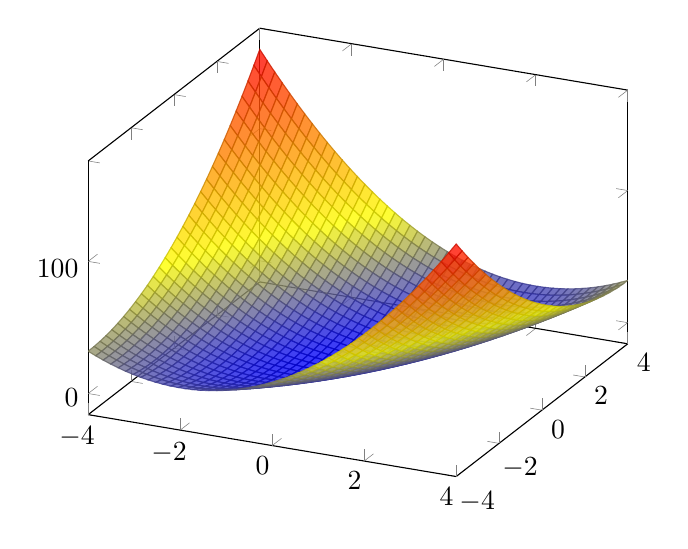
\begin{tikzpicture}
				\begin{axis}
					\addplot3[
					surf,
					opacity=0.8,
					samples=50, samples y=30,
					%samples=80, samples y=50,
					%colormap/whitered,
					%domain=-1:1,domain y=-2:6
					%domain=4:12,domain y=-20:-5
					domain=-4:4,domain y=-4:4
					%z buffer=sort,
					]
					%{x^2 - 4*x*y + y^2};
					%{2*x^2 - 1*x*y + 2*y^2 - x - 2*y};
					%{sin(0.5*x^2 - 0.25*y^2 + 3) * cos(2*x - exp(y) + 1)};
					%{4*x^2 + 5*x*y + 2*y^2 - 4*x + 12*y};
					{4*x^2 - 4*x*y + 2*y^2};
				\end{axis}
			\end{tikzpicture}
			\caption{Beispiel einer Hyperfläche.}
		\end{figure}
	}


	\newpage
	\methode{
		\n 
		In jeder Iteration dieses Verfahrens berechnet man folgende 3 Schritte:
		\begin{enumerate}
			\item Aktuelles Residuum: ("Schrittrichtung") 
			\begin{align} 
 				r\st{k} = b - Ax\st{k} 
 			\end{align}
			\item Optimale Schrittweite:
			\begin{align} 
 				\alpha\st{k} = \frac{r^{(k)\trans} \cdot r\st{k}}{r^{(k)\trans} \cdot A r\st{k}} 
 			\end{align}
			\item Aktuelles Zwischenergebnis:
			\begin{align} 
 				x\st{k+1} = x\st{k} + \alpha\st{k} \cdot r\st{k} 
 			\end{align}
		\end{enumerate}
	}

	\sbreak
	\bsp{
		\n 
		Sei folgendes LGS (aus obigem Beispiel) gegeben und der Startvektor $x\st{0} = (0, 0)\trans$
		\begin{align*}
			\begin{bmatrix}
				1 & 3 \\
				2 & 2
			\end{bmatrix} \cdot 
			\nvector{
				x_0 \\ x_1
			} = 
			\nvector{
				2 \\ 2
			}
		\end{align*}
		Wir berechnen die erste Iteration nach obiger Methode:
		\begin{align*}
			&r^{(0)} = b - Ax^{(0)} = 
			\nvector{
				2 \\ 2
			} \\
 			\alpha^{(0)} &= \frac{r^{(0)\trans} \cdot r^{(0)}}{r^{(0)\trans} \cdot A r^{(0)}} = \frac{8}{32} = \frac{1}{4} \\ 		
			x\st{1} = x\st{0} &+ \alpha\st{0} \cdot r\st{0} = (0, 0)\trans + \frac{1}{4} \cdot 
			\nvector{
				2 \\ 2
			} = \frac{1}{2} 
			\nvector{
				1 \\ 1
			}
		\end{align*}
		Hier käme die nächste Iteration und erfolgt völlig analog\dots
	}

	\newpage
	\defi{
		\n 
		Grafisch wird dieses Verfahren häufig so dargestellt, indem man die Höhenlinien der Hyperfläche als Kreise einzeichnet. Höhenlinien, weil ein Kreis bedeutet, dass alle Punkte auf dieser Kreislinie dieselbe Höhe (y-Wert) besitzen.
		\n 
		Das Verfahren konvergiert schneller, je gleichmäßiger es nach außen geht. Um genau zu sein braucht das Verfahren genau ein Schritt, falls die grafische Darstellung der Funktion (also die Höhenlinien) konzentrische Kreise bilden, also die Hyperfläche einem umgedrehten Kegel entspricht.
		\n 
		In der Praxis gleicht die grafische Darstellung meist eher weiten Ellipsen, weswegen dieses Verfahren genau so in der Praxis häufig recht langsam ist. Es gibt aber eine bessere Variante, das sogenannte "Conjugated gradient descent" (online nachschauen, wenn das Interesse geweckt hat).
	%}
	%
		\begin{figure}[H]
			\centering
				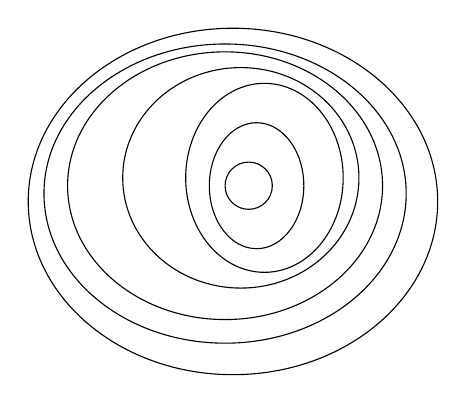
\begin{tikzpicture}
					\draw (0,0) ellipse (0.3cm and 0.3cm);
					\draw (0.1,0) ellipse (0.6cm and 0.8cm);
					\draw (0.2,0.1) ellipse (1.0cm and 1.2cm);
					\draw (-0.1,0.1) ellipse (1.5cm and 1.4cm);
					\draw (-0.3,0.0) ellipse (2.0cm and 1.7cm);
					\draw (-0.3,-0.1) ellipse (2.3cm and 1.9cm);
					\draw (-0.2,-0.2) ellipse (2.6cm and 2.2cm);
				\end{tikzpicture}
			\caption{Beispielhafte grafische Darstellung eines "steepest descent" Problems.}
		\end{figure}
		\noindent Die Schrittrichtung in einem Schritt ist dann einfach immer senkrecht zur momentanen Höhenlinie, da es der jeweils steilste Abstieg in dem Punkt ist.
%		Ein Bild hierzu wäre: \\
	}
	
%		Die Schrittrichtung ist immer senkrecht zur momentanen Höhenlinie.
%		%An diesem Bild sieht man auch schön grafisch, was bei den einzelnen Schritten passiert. Die Schrittrichtung entspricht immer senkrecht zur aktuellen "Höhenlinie", auch wenn diese natürlich nicht eingezeichnet ist. Gerade beim ersten Schritt, wo der Startpunkt genau auf einer Linie ist, kann man sehr gut erkennen, dass die Schrittrichtung orthogonal zu der Linie ist.
%		%\n 
%		%Und beim vierten Schritt (also von $x_3$ aus) erkennt man auch super, dass die Linie orthogonal zur Schrittrichtung ist.
%	}
          % Fixpunktiteration für LGS
		

	\newpage
% =========================================================	
	\section{Eigenwertproblem}
% =========================================================
	
	\sbreak
	\defi{
		\n 
		Eigenwerte kennt man vermutlich noch aus DS und Lineare Algebra. Wir wiederholen diese kurz und beschäftigen uns mit iterativen Verfahren, welche diese Art von Problem lösen.
		\n
		Wir haben eine Matrix $A$, einen Vektor $v$ und einen Skalar $\lambda$ und
		\begin{align} 
 			Av = \lambda v 
 		\end{align}
		$v$ bezeichnet man hierbei als einen Eigenvektor und $\lambda$ einen Eigenwert von $A$.
		\n 
		Formell bezeichnet ein Eigenvektor einer Abbildung ein vom Nullvektor verschiedener Vektor, dessen Richtung durch die Abbildung nicht verändert wird. Ein solcher Eigenvektor wird durch die Abbildung lediglich skaliert. Dieser Faktor ist der Eigenwert.
		\n 
		Ein typisches Beispiel wäre die Scherabbildung.%: \url{https://de.wikipedia.org/wiki/Scherung_(Geometrie)}
	}

	\sbreak
	\methode{ \n 
		Wie rechnet man pauschal einen Eigenvektor und -wert aus? \\
		Gegeben sei eine Matrix $A$:
		\begin{align} 
 			\det(A - \lambda_i \unitM) = 0 
 		\end{align}
		Mit $\unitM$ als Einheitsmatrix, löse obige Gleichung, um auf alle Eigenwerte zu schließen. Mithilfe obiger Ausgangsbedingung
		\begin{align*} 
 			Av = \lambda v 
 		\end{align*}
		leiten wir folgende Beziehung ab, um die Eigenvektoren auszurechnen:
		\begin{align} 
 			(A - \lambda_i \unitM)\cdot v_i = 0 
 		\end{align}
		%Diese Gleichung können wir mithilfe von Gauß-Elimination lösen, da sie einem LGS entspricht. Beim Ausrechnen eines Eigenvektors haben wir immer \fat{einen Freiheitsgrad}, sprich es entsteht immer eine Nullzeile beim Gauß-Verfahren. Das liegt daran, dass wir nur an der Richtung des Eigenvektors interessiert sind, nicht dessen Länge. %was wiederum bedeutet, dass wir einmalig pro Ausrechnen eines Eigenvektors einen Eintrag beliebig wählen können und dann alle anderen Komponenten im Abhängigkeit dazu.
	}

	\newpage
	\defi{
		\n 
		Die Gleichung zum Ausrechnen des Eigenvektors können wir mithilfe von Gauß-Elimination lösen, da sie einem LGS entspricht. Beim Ausrechnen eines Eigenvektors haben wir immer \fat{einen Freiheitsgrad}, es entsteht immer eine Nullzeile beim Gauß-Verfahren. Das liegt daran, dass wir nur an der Richtung des Eigenvektors interessiert sind, nicht dessen Länge.
		\n 
		Wir können also (wie immer bei Freiheitsgraden), sobald wir bei der Nullzeile sind, einen Wert des Vektors festlegen und alle anderen anhand des festgelegten berechnen. Es gibt also im Prinzip unendlich viele Lösungen, aber jeder Lösungsvektor ist nur ein Vielfaches eines anderen Lösungsvektors.
		\n 
		In der Praxis würde man den Vektor so bestimmen, dass die Norm Eins beträgt.
	}

	\sbreak
	\bsp{ Eigenwerte: 
		\begin{align*}
			A &= 
			\begin{bmatrix}
				1 & 0  \\
				2 & 2 
			\end{bmatrix} \\
			\text{charakteristisches Polynom} := (A &- \lambda \unitM) = 
			\begin{bmatrix}
				1 - \lambda & 0 \\
				2 & 2 - \lambda
			\end{bmatrix} \\
 			\det(A - \lambda \unitM) &= (1 - \lambda) \cdot (2 - \lambda) \\
			0 &= 2 - \lambda - 2\lambda + \lambda^2 \\
			0 &= 2 - 3\lambda + \lambda^2
 		\end{align*}
		P-Q Formel bzw. Mitternachtsformel\dots
		\begin{align*} 
 			\lambda_1 &= 1 \\
			\lambda_2 &= 2 
 		\end{align*}
	}

	\newpage
	\bsp{ Eigenvektoren:
		\n 
		Obiges Beispiel weitergeführt, wir möchten die Eigenvektoren zu obigem $A$ erhalten.
		\begin{align*} 
 			(A-\lambda_i \unitM)\; v_i = 0 
 		\end{align*}
		Für beliebigen Eigenwert umgesetzt:
		\begin{align*}
			\begin{bmatrix}
				1 - \lambda_i & 0 & | & 0  \\
				2 & 2 - \lambda_i & | & 0
			\end{bmatrix}
		\end{align*}
		Für $\lambda_1 = 1$ eingesetzt:
		\begin{align*}
			\begin{bmatrix}
				0 & 0 & | & 0  \\
				2 & 1 & | & 0
			\end{bmatrix}
		\end{align*}
		Hier sehen wir den einen Freiheitsgrad. Wir setzen (beispielsweise) die zweite Komponente auf $1$. Es ergibt sich der Lösungsvektor und damit Eigenvektor des ersten Eigenwertes von $A$:
		\begin{align*} 
 			v_1 = 
 			\nvector{
	 			\nicefrac{-1}{2} \\
	 			1
 			}
 		\end{align*}
	}


	\sbreak
	\subsection{Kondition}
	
	\methode{
		\n 
		Um die Kondition eines Eigenwert- und Eigenvektorproblems zu bestimmen gehen wir davon aus, dass die Einträge der Matrix $A$ einen fehlerhaften Offset von $\epsilon$ besitzen. Wie sonst auch immer rechnen wir den Algorithmus einfach mit beliebigem, nicht festem Fehler $\epsilon$ aus und schauen uns an, wie stark sich der Fehler auf die Ausgabe auswirkt.
	}

	%	TBD
	%}


	\newpage
	\subsection{Rayleigh Quotient}
	
	\defi{
		\n 
		Der Rayleigh Quotient ist eine Möglichkeit, einen Eigenwert einer Matrix $A$ mit gegebenem Eigenvektor $v$ "einfach" auszurechnen.
		\\
		Herleitung:
		\begin{align*} 
 			A \cdot v &= \lambda v \\
			v\trans \cdot A \cdot v &= \lambda \cdot v\trans \cdot v \\
			\lambda &= \frac{v\trans\cdot A \cdot v}{v\trans \cdot v} 
 		\end{align*}
	}

	\sbreak
	\methode{
		\n 
		Sei $v \in \Re^n$ ein Eigenvektor einer Matrix $A \in \reals^{n \times n}$. Der Eigenwert $\lambda$ zu diesem Eigenvektor $v$ der Matrix $A$ kann wie folgt berechnet werden:
		\begin{align} 
 			\lambda = \frac{v\trans\cdot A \cdot v}{v\trans \cdot v} 
		\end{align}
	}

	\sbreak
	\bsp{
		\n 
		Obiges Beispiel:
		\begin{align*}
			A = 
			\begin{bmatrix}
				1 & 0  \\
				2 & 2 
			\end{bmatrix} 
			\quad \quad
			v_1 = 
			\nvector{
				\nicefrac{-1}{2} \\
				1
			}
		\end{align*}
		Rayleigh Quotient nutzen, um auf den Eigenwert zu schließen:
		\begin{align*}
			\lambda &= 
				\frac{
					\nvector{
						-\frac{1}{2} & 1
					} 
					\cdot 
					\begin{bmatrix}
						1 & 0  \\
						2 & 2 
					\end{bmatrix}
					\cdot 
					\nvector{
						\nicefrac{-1}{2} \\
						1
					}
				}{ % frac
					\nvector{
						-\frac{1}{2} & 1
					} 
					\cdot
					\nvector{
						\nicefrac{-1}{2} \\
						1
					}
				} \\
			&= \frac{
					\nvector{
						1.5 & 2
					}
					\cdot 
					\nvector{
						\nicefrac{-1}{2} \\
						1
					}
				}{ % frac
					\nicefrac{5}{4}
				} \\
			&= \frac{\l(\nicefrac{-3}{4} + 2 \r) \cdot 4}{5} \\
			&= \frac{1}{4} \cdot 4 = 1
			%&= 1
		\end{align*}
		Stimmt, wie die vorherigen Beispielboxen zeigen \Laughey.
	}


	\newpage
	\subsection{Vektor-/Poweriteration}
	
	\sbreak
	\defi{ \n 
		Die sogenannte Poweriteration ist ein Verfahren, welches Eigenwerte annähern kann. Um genau zu sein, wirft man in diesen Algorithmus die Matrix $A$ und einen Startvektor $x_0$. Dieser $x$-Vektor wird sich mit jeder Iteration dem Eigenvektor für den betragsmäßig größten Eigenwert von $A$ annähern.
	}

	\lbreak
	\subsubsection{Direct Power Iteration}
	
	\methode{\n 
		Die Iterationsvorschrift der Power-Iteration:
		\begin{align} 
 			x_{k+1} = \frac{A \cdot x_k}{\norm{A \cdot x_k}} 
 		\end{align}
		Der untere Teil des Bruchstrichs bedeutet einfach nur, dass nach jedem Schritt der Vektor wieder normalisiert wird.
	}

	\sbreak
	\defi{ \n 
		Das Verfahren hat aus dem Grund seinen Namen, weil man das ganze auch rekursiv formulieren kann. Dann wäre es:
		\begin{align}
		x_{k+1} = A^k \cdot x_0
		\end{align}
		Dann würde man erst danach normalisieren. Die Normalisierung in jedem Schritt (siehe iterative Formel) macht man eh nur aus Stabilitätsgründen, da ansonsten die Zahlen immer größer werden was bei unserer Arithmetik tendenziell zu größeren Fehlern führt.
		\n 
		Da man auch am Eigenwert interessiert ist, nutzt man den Rayleigh Quotient um aus einer Power Iteration Approximation eines Eigenvektors den zugehörigen Eigenwert zu erhalten.
		\begin{align} 
			\lambda_{k+1} = \frac{x_{k}\trans\cdot A \cdot x_{k}}{x_{k}\trans \cdot x_{k}} 
		\end{align}
	}

	\newpage
	\subsubsection{Shifted Power Iteration}
	
	\defi{ \n 
		Man kann aber auch noch einen sogenannten \fat{Shift} $\mu$ einbauen. Mittels Shift kann die Matrix so manipuliert werden, dass die Eigenwerte um den Shift verschoben werden. Dadurch kann man erreichen, dass nun andere Eigenwerte der maximale Eigenwert sind und das Verfahren konvergiert gegen den entsprechend anderen Eigenwert. \n
		Dieser Shift verschiebt im Grunde alle Eigenwerte um denselben Betrag nach unten. Also die Eigenwerte $\lambda_1 = 3$ und $\lambda_2 = 4$ mit einem Shift von $\mu = 4$ würden zu $-1$ und $0$ werden. Mit diesem Shift würde die Power Iteration zu ersterem Eigenwert konvergieren, da dieser mit dem Shift der \fat{betragsmäßig} größte ist.
	}

	\sbreak
	\methode{ \fat{Shifted Power Iteration}
		\begin{align} 
 			x_{k+1} = \frac{(A - \mu \cdot \unitM) \cdot x_k}{\norm{(A - \mu \cdot \unitM) \cdot x_k}} 
 		\end{align}
		Im Grunde genommen ist dieser Shift also ein konstanter Offset aller Diagonaleinträge von $A$ jeder Iteration.
	}

	\sbreak
	\defi{ \n 
		Wenn wir einen Shift haben müssen wir das beim Ausrechnen des Eigenwertes berücksichtigen und dessen Auswirkung rückwirkend mitberechnen. Wir müssen dann die Formel für den Rayleigh Quotient wie folgt anpassen:
		\begin{align} 
		\lambda_{k+1} = \frac{x_{k}\trans\cdot (A - \mu \cdot \unitM) \cdot x_{k}}{x_{k}\trans \cdot x_{k}} + \mu
		\end{align}
	}

	\sbreak
	\wichtig{\n 
		Wenn zwei Eigenwerte durch den Shift \fat{betragsmäßig} am größten sind, konvergiert die Power Iteration gar nicht mehr!
	}


	\newpage
	\bsp{\n
		Wir führen eine Power-Iteration über die folgende Matrix $A$ durch.
		\begin{align*}
			A = \nmatrix{2 & 2 \\ 4 & 0}
		\end{align*}
		Als Startvektor sei $x_0 = \nvector{1 \\ 0}$ gegeben.
		\n
		Zwei Schritte mit einem Shift $\mu = 0$:
		\begin{align*}
			x_1 &= A \cdot x_0 \\
				&= \nmatrix{2 & 2 \\ 4 & 0} \cdot \nvector{1 \\ 0} \\
				&= \nvector{2 \\ 4} \\
				&\\
			x_2 &= A \cdot x_1 \\
				&= \nmatrix{2 & 2 \\ 4 & 0} \cdot \nvector{2 \\ 4} \\
				&= \nvector{12 \\ 8}
		\end{align*}
		Dies würde sich (normiert) dem Vektor $(1, 1)\trans$ annähern, welche der Eigenvektor zu dem Eigenwert $\lambda_2 = 4$ ist, welcher der betragsmäßig größte von $A$ ist.
		\n
		Zwei Schritte mit einem Shift $\mu = 2$:
		\begin{align*}
		(A - \mu \unitM) &= \nmatrix{2-2 & 2 \\ 4 & 0-2} \\
		x_1 &= \nmatrix{0 & 2 \\ 4 & -2} \cdot \nvector{1 \\ 0} \\
			&= \nvector{0 \\ 4} \\
			&\\
		x_2 &= \nmatrix{0 & 2 \\ 4 & -2} \cdot \nvector{0 \\ 4} \\
			&= \nvector{8 \\ -8}
		\end{align*}
	}
	
	\newpage
	\subsubsection{Konvergenzrate}
	
	\defi{\n 
		Die \fat{Konvergenzrate} der direkten Power Iteration sagt aus, wie schnell sich der Algorithmus der exakten Lösung annähert. Sie ist definiert als:
		\begin{align} 
 			q = \abs{\frac{\lambda_2 - \mu}{\lambda_1 - \mu}} \qquad \in [0, 1]
 		\end{align}
		Dabei ist $\lambda_2$ der betragsmäßig zweitgrößte und $\lambda_1$ der größte Eigenwert von $A$, den Shift jeweils schon einberechnet (verwirrend? Guck dir unten das Beispiel an!). 
		\n
		Die Eigenvektoren konvergieren linear (also quasi $\epsilon_{k+1} = \epsilon_{k} \cdot q$; mit $\epsilon$ als den Fehler) und die Eigenwerte quadratisch mit diesem Faktor. 
		Aus diesem Grund ist das direkte Verfahren schlecht geeignet, wenn man viele Eigenwerte nahe dem maximalen Eigenwert hat. $q$ geht hierbei gegen 1. Die Konvergenzrate liegt immer zwischen $1$ und $0$, wobei $0$ Perfektion wäre, aka es konvergiert mit einem Schritt auf die analytisch korrekte Lösung.
	}

	\sbreak
	\bsp{\n
		Man hätte zwei Eigenwerte $3$ und $12$ und einen Shift von $\mu = 2$. Dadurch wäre der betragsmäßig größte Eigenwert $12-2$ und der zweitgrößte $3-2$ (mit dem Shift angegeben). Wir erhalten:
		\begin{align*}
			q = \abs{\frac{3 - 2}{12 - 2}} = \frac{1}{10}
		\end{align*}
		Das würde im Grunde also bedeuten, dass jede Power Iteration eine Dezimalstelle genauer wird.
		\n
		Nehmen wir nun $\mu = 6$. Wir erhalten:
		\begin{align*}
			q = \abs{\frac{3 - 6}{12 - 6}} = \frac{3}{6} = \frac{1}{3}
		\end{align*}
		Obwohl mit beiden Shifts die Power Iteration zu demselben Eigenwert konvergiert, hat der Shift einen Einfluss auf die Konvergenzgeschwindigkeit!
		\n
		Wählen wir dagegen $\mu > 7.5$, also beispielsweise $\mu = 10$, wird $3$ zum betragsmäßig größtem Eigenwert. Wir erhalten:
		\begin{align*}
			q = \abs{\frac{12 - 10}{3 - 10}} = \frac{2}{7}
		\end{align*}
	}

	\newpage
	\subsubsection{Inverse Power Iteration}
	
	\defi{ \n 
		Natürlich gibt es dieses Verfahren noch invertiert. Hierbei konvergiert das Verfahren gegen den Eigenvektor des betragsmäßig \fat{kleinsten} Eigenwertes von $A$.
	}

	\sbreak
	\methode{\n 
		Mit
		\begin{align} 
 			B = (A - \mu \cdot \unitM)\inv
 		\end{align}
		ergibt sich die Iterationsvorschrift:
		\begin{align} 
 			x_{k+1} = \frac{B \cdot x_k}{\norm{B \cdot x_k}} 
 		\end{align}
	}

	\sbreak
	\defi{ \n 
		Im obigen Methodenblock ist die Inverse Power-Iteration direkt mit Shift $\mu$ eingebaut worden, welcher analog zur nicht inversen Variante funktioniert. \\
		Damit lassen sich dann ein paar nette Tricks machen. Möchte man den betragsmäßig kleinsten Eigenwert haben, lässt man die Inverse mit einem Shift von $\mu = 0$ laufen. Weiß man z.B., dass man drei Eigenwerte hat und den mittleren haben will, kann man die Inverse Power Iteration mit einem Shift von $0.5 \cdot (\lambda_1 + \lambda_2)$ laufen lassen. 
		Durch das Benötigen der Inverse einer Matrix ist diese Methode aber laufzeit-technisch aufwändiger.
	}
	
           % Eigenwertproblem + Power Iteration

% ---------------------------------------------------------------------------
% Differentialgleichungen
% ---------------------------------------------------------------------------
	
	\newpage
% =========================================================	
	\section{Differentialgleichungen}
% =========================================================
	
	\sbreak
	\defi{
		\n 
		Differentialgleichungen, ernsthaft? Man weiß häufig nur, dass diese kompliziert, schwer zu lösen und nervig sind. Da dies (meiner Meinung nach) nicht stimmt, zeige ich dies folgendermaßen:
		\n 
		Eine "gewöhnliche Differentialgleichung" ist eine Gleichung, die eine Funktion durch ihre Ableitung beschreibt:
		\begin{align} 
 			y'(t) = \varphi(y,t) 
 		\end{align}
		Ein Beispiel wäre eine Sonnenblume, die proportional zu ihrer momentanen Größe wächst:
		\begin{align*} 
 			y'(t) = 2y(t) 
		\end{align*}
		Die Lösung eines solchen Systems ist eine Funktion $y(t)$. In diesem Falle würde es die Größe der Blume in Abhängigkeit zu einem Zeitpunkt $t$ angeben.
		\n 
		Doch wie löst man ein solches ODE? ("ordinary differential equation")
	}
	
	\lbreak
	\subsection{Separation der Variablen}
	
	\methode{
		\n 
		Gegeben ist eine Differentialgleichung der Form
		\begin{align*} 
 			y'(t) = \varphi(y,t) 
 		\end{align*}
		Methodik:
		\begin{enumerate}
			\item In Leibniz-Notation schreiben
			\item Separieren
			\item Integrieren
			\item Integrale lösen
			\item Nach y auflösen
		\end{enumerate}
	}

	\newpage
	\bsp{
		\n 
		Mit obiger Methode ergibt sich für unser Beispiel folgende Rechnung:
		\begin{align*} 
 			y'(t) = 2y(t) 
 		\end{align*}
		In Leibniz Notation schreiben:
		\begin{align*}
 			\frac{\d y}{\d t} = 2y 
 		\end{align*}
		Separieren der Variablen:
		\begin{align*} 
 			\frac{\d y}{2y} = \d t 
 		\end{align*}
		Integrieren:
		\begin{align*} 
 			\int_{y_0}^{y}\frac{1}{2\eta}\d\eta = \int_{t_0}^{t}\d\tau 
 		\end{align*}
		Lösen und nach y(t) auflösen:
		\begin{align*} 
 			\frac{1}{2}\l(\ln\abs{y} - \ln\abs{y_0}\r) &= t - t_0 \\
 			\abs{\frac{y(t)}{y_0}} &= e^{2(t - t_0)} \\
			y(t) &= \pm y_0 \cdot e^{2(t - t_0)} 
 		\end{align*}
		Dies nennt man die allgemeine Lösung des ODEs, da die Funktion für alle $y_0$ und alle $t_0$ die Differentialgleichung erfüllt.
	}

	\sbreak
	\subsection{Verkürzte Version}
	
	\methode{ \n 
		Folgende umgeschriebene Variante ist ein Versuch, die Separation der Variablen schöner darzustellen:\\
		Gegeben ist eine Differentialgleichung der Form
		\begin{align} 
 			y'(t) = f(t) \cdot g(y(t)) 
 		\end{align}
		Man stellt folgende Gleichung auf:
		\begin{align} 
 			\int_{y_0}^{y}\frac{1}{g(y(\eta))}\d\eta = \int_{t_0}^{t} f(\tau)\d\tau 
 		\end{align}
		Nun löst man die entstandene Gleichung nach $y(t)$ auf und ist fertig.
	}

	\newpage
	\bsp{\n 
		Obiges Beispiel: 
		\begin{align*} 
 			y'(t) = 2y(t) 
 		\end{align*}
		Nach der Methodik ist $f(t) = 2$ und $g(y(t)) = y(t)$ \\
		Gleichung aufstellen:
		\begin{align*} 
 			\int_{y_0}^{y}\frac{1}{\eta}\d\eta &= \int_{t_0}^{t}2 \d\tau \\
			(\ln\abs{y} - \ln\abs{y_0}) &= 2 \cdot (t - t_0) \\
			y(t) &= \pm y_0 \cdot e^{2(t - t_0)} 
 		\end{align*}
	}

	\sbreak
	\defi{\n 
		$y_0$ und $t_0$ sind sogenannte Anfangsbedingungen. 
		\n
		Wenn man sie gegeben hat, löst man ein sogenanntes \fat{AWP (=Anfangswertproblem)}. Hierzu muss man die allgemeine Lösung des ODEs in die spezifische übertragen, bei der man schlichtweg $y_0$ und $t_0$ einsetzt. \\
		Solche Anfangsbedingungen könnten z.B. $t \ge 0$ und $y(0) = 1$ sein.
		\n 
		$t_0$ beschreibt den niedrigsten, noch gültigen Wert für $t$. Da $t$ meist die Zeit beschreibt, ist es logisch, dass diese z.B. bei dem Wachstum einer Blume nicht im negativen anfängt.
		\n 
		Außerdem beschreibt $y_0$ den Wert am Startzeitpunkt $t_0$:
		\begin{align} 
 			y(t_0)=y_0 
 		\end{align}
	}

	\newpage
	\bsp{\n 
		Obiges Beispiel, obige Anfangsbedigungen, also: \\
		ODE:
		\begin{align*} 
 			y'(t) = 2y(t) 
 		\end{align*}
		Allgemeine, also Lösung des ODE:
		\begin{align*} 
 			y(t) = \pm y_0 \cdot e^{2(t - t_0)} 
 		\end{align*}
		Anfangsbedingungen:
		\begin{align*} 
 			t \ge 0 &\longrightarrow t_0 = 0 \\
			y(0) = 1 &\longrightarrow y_0 = 1 
 		\end{align*}
		Spezifische, also Lösung des AWP:
		\begin{align*} 
 			y(t) &= 1 \cdot e^{2t} \\
 				&= e^{2t}
 		\end{align*}
	}

	\sbreak
	\subsection{Kleiner Trick}
	\label{chap:ode_trick}
	
	\methode{\n 
		Wenn ihr ein ODE habt, welches nicht von $t$ abhängig ist, sprich in folgender Form ist:
		\begin{align} 
 			y'(t) = a \cdot y(t) \aae a\in \Re 
 		\end{align}
		Dann ist die Lösung des ODEs \fat{immer}:
		\begin{align} 
 			y(t) = y_0 \cdot e^{a \cdot (t-t_0)} 
 		\end{align}
	}

	\newpage
	\vertief{ \n 
		Für die Interessierten hier der Beweis für \ref{chap:ode_trick}:
		\begin{align*} 
 			y'(t) = a \cdot y(t) 
 		\end{align*}
		Mit obiger verkürzter Variante der Separation der Variablen:
		\begin{align*} 
 			\int_{y_0}^{y}\frac{1}{y(\eta)} \d\eta &= \int_{t_0}^{t}a \cdot \d\tau \\
			\ln\abs{y} - \ln \abs{y_0} &= a \cdot \int_{t_0}^{t} \d\tau = a \cdot (t - t_0) \\
			\ln \l(\abs{\frac{y}{y_0}} \r) &= a \cdot (t - t_0) \\ \\
			y(t) &= y_0 \cdot e^{a \cdot (t-t_0)} 
 		\end{align*}
	}

	\newpage
	\subsection{Kondition eines AWPs}
	
	\defi{\n
		Um die Kondition eines Anfangswertproblems zu untersuchen, betrachten wir die Relation von einem Eingabe- und Ausgabefehlers. Bei einem AWP wäre der Eingabewert der Startwert $y_0$, während die Ausgabe die Funktion $y(t)$ entspricht.
	}

	\sbreak
	\bsp{\n
		Gegeben sei das exakte Ergebnis eines AWPs:
		\begin{align*}
			y(t) = y_0 \cdot e^{4t}
		\end{align*}
		mit $y_0 = 3$.
		Dann definieren wir uns eine verfälschte Eingabe $y_\epsilon = y_0 + \epsilon$. Dadurch wird die nun verfälschte Ausgabe zu:
		\begin{align*}
			y_\epsilon(t) &= y_\epsilon \cdot e^{4t} \\
				&= (y_0 + \epsilon) \cdot e^{4t} \\
				&= y_0 \cdot e^{4t} + \epsilon \cdot e^{4t}\\
				&= y(t) + \epsilon  \cdot e^{4t}\\
		\end{align*}
		Der Ausgabefehler an sich ist der Teil, der die korrekte Lösung verfälscht. Diese untersuchen wir dann für $t$ geht gegen unendlich.
		\begin{align*}
			\lim\limits_{t\rightarrow\infty}\l( \epsilon  \cdot e^{4t} \r) = \infty
		\end{align*}
		Das untersuchte AWP ist also schlecht konditioniert.
	}

	\newpage
	\subsection{(Explizite) Einschrittverfahren}
	
	\defi{
		\n 
		Einschrittverfahren bieten die Möglichkeit, ODEs schrittweise anzunähern.
		Im Folgenden sei $\delta t$ immer unsere Schrittweite, also in wie große (oder grobe) Stücke wir (die Zeit) $t$ unterteilen.
		\n 
		Bevor wir uns drei explizite Verfahren anschauen, wäre es wichtig, die grafische Darstellung eines ODE zu verstehen:
	}

	\lbreak
	\subsubsection{Richtungsfelder}
	
	\defi{
		\n 
		Richtungsfelder bieten die Möglichkeit, das ODE graphisch anschaulich darzustellen. Hierfür stellen wir lediglich ein Graph mit $x$ und $y(t)$ als Achsen auf. Punkte dieses Graphen stellen jeweils Werte der Ableitung da. Dafür ziehen wir bei jedem Punkt eine kleine Linie, welche die Steigung widerspiegelt. \\
		Also wenn unser ODE $y'(t) = x^2 + y$ wäre, würden folgende Punkte folgende Steigungen haben: \\
		$P(0, 1) \imp 0^2 + 1 = 1$ hätte die Steigung 1. \\
		$Q(1, 2) \imp 1^2 + 2 = 3$ hätte die Steigung 3. \\
		$R(2, 0) \imp 2^2 + 0 = 4$ hätte die Steigung 4 und so weiter und so fort.
		\n 
		Zeichnet man genug dieser kleinen Linien in den Graphen kann man einen "Strom" erkennen, der auf die Lösung des ODEs vermuten lässt.
%		Hier ist ein gutes Video, dass dies schön mit Bildern erklärt:\\
%	}
%%
%					axis lines=middle,
%					xlabel=$t$,
%					ylabel=$y(t)$,
%					enlargelimits,
%					legend pos=outer north east,
%					%ymin=-0.3,
%					%xmax=5.8,
%					%xticklabels={,,},
%					%yticklabels={,,},
%					]
%					%\tikzPointUp{$f(1)$}{1,0}
%					%\tikzPointDown{$f(2)$}{2,2}
%%					
%					%\tikzDeriveLine{2}{0}{4}%{0.5}
%					%\tikzDeriveLine{3}{0}{6}%{0.5}
%					%\tikzDeriveLine{4}{0}{8}%{0.5}
%%
		\n 
		Wenn man jetzt (informell) einem Strom mit einem Stift folgt, zeichnet man eine mögliche Stammfunktion ein, welche das ODE erfüllt. Bedenke ja, dass man bei Stammfunktionen immer den konstanten Offset $c$ hat, der beliebig sein kann. Und deswegen gibt es unendlich viele Pfeile im Richtungsfeld, denen man folgen kann und die trotzdem eine Lösung bilden.
		\n 
		Wenn man beispielsweise von der Funktion 
		\begin{align*} 
 			y'(t) = 2t 
 		\end{align*} 
 		das Richtungsfeld einzeichnen würde, könnte man ganz viele, vertikal verschobene Parabeln erkennen. Logisch, das Integral von $y'(t)$ ist:
		\begin{align*} 
 			y(t) = t^2 + c 
 		\end{align*}
		Und genau dieses Prinzip nutzen wir jetzt für Schrittverfahren, die nichts anderes tun als Ableitungen (die Linien im Richtungsfeld) in Punkten zu nutzen, um einen Schritt auszurechnen (grafisch könnte man sagen, sie laufen den Pfeilen hinterher).
	}

	\sbreak
	\defi{
		\n 
		Für den Rest des Kapitels beschreibt $f(t_k, y_k)$ die Funktion, welche zu diskreten Zeitpunkten $t_k$ und Werte $y_k$ die Ableitung berechnet. Im Grunde ist es also nichts anderes als die rechte Seite des ODEs.
		\n 
		1. Beispiel:
		\begin{align*}
			y_0'(t) &= 2 y(t) \\
			f_0(t_k, y_k) &= 2 y_k \\
		\end{align*}
		2. Beispiel:
		\begin{align*}
			y_1'(t) &= 4t \cdot 2y(t) \\
			f_1(t_k, y_k) &= 4 t_k \cdot 2 y_k
		\end{align*}
	}


	\newpage
	\subsubsection[Explizites Euler-Verfahren]{Explizites Euler-Verfahren (1. Ordnung)} \label{chap:explizitSchrittverfahren}
	
	\methode{
		\n 
		Bei diesem Verfahren wird die Steigung im aktuellen Punkt $t_k$ der Iteration zur Berechnung der nächsten Annäherung genutzt.
		\begin{align} 
 			t_k = t_0 + k \cdot \delta t 
 		\end{align}
		\begin{align} 
 			y_{k+1} = y_k + \delta t \cdot f(t_k, y_k) 
 		\end{align}
	}

	\sbreak
	\subsubsection[Heun-Verfahren]{Heun-Verfahren (2. Ordnung)}
	
	\methode{
		\n 
		Bei diesem Verfahren wird die Steigung in zwei Punkten (analog zur Trapezregel aus der Quadratur) der Iteration zur Berechnung der nächsten Annäherung genutzt.
		\begin{align} 
 			t_k = t_0 + k \cdot \delta t 
 		\end{align}
		\begin{align} 
 			y_{k+1} = y_k + \frac{\delta t}{2} \cdot \l(f(t_k, y_k) + f(t_{k+1}, y_k + \delta t \cdot f(t_k, y_k))\r) 
 		\end{align}
	}

	\sbreak
	\subsubsection[Runge-Kutta Verfahren]{Runge-Kutta Verfahren (4. Ordnung)}
	
	\methode{
		\n 
		Hier wird analog zur Simpsonregel aus der Quadratur noch mehr Punkte für die Iteration genutzt.
		\begin{align} 
 			t_k = t_0 + k \cdot \delta t 
 		\end{align}
		\begin{align} 
 			T_1 &= f(t_k, y_k) \\
			T_2 &= f \l(t_k + \frac{\delta t}{2}, y_k + \frac{\delta t}{2} T_1 \r) \\
 			T_3 &= f \l(t_k + \frac{\delta t}{2}, y_k + \frac{\delta t}{2} T_2 \r) \\
 			T_4 &= f \l(t_{k+1}, y_k + \delta t \cdot T_3 \r) 
 		\end{align}
		\begin{align} 
 			y_{k+1} = y_k + \frac{\delta t}{6} \cdot (T_1 + 2T_2 + 2T_3 + T_4) 
 		\end{align}
	}
	
	\newpage
	\bsp{
		\n 
		Euler-Verfahren: \\
		Wir haben die Startwerte $y_0 = 1 \aae t_0 = 0$, außerdem ist $\delta t = 1$ und unser ODE:
		\begin{align*} 
 			y'(t) = 2y(t) 
 		\end{align*}
		Unsere Funktion ist also 
		\begin{align*} 
 			f(t_k, y_k) = 2y_k 
 		\end{align*}
		1. Schritt:
		\begin{align*} 
 			t_1 &= t_0 + k \cdot \delta t = 0 + 1 \cdot 1 = 1 \\
 			y_1 &= y_0 + \delta t \cdot 2y_0 = 1 + 1 \cdot 2 \cdot 1 = 3 
 		\end{align*}
		2. Schritt:
		\begin{align*} 
 			t_2 &= t_0 + k \cdot \delta t = 0 + 2 \cdot 1 = 2 \\
			y_2 &= y_1 + \delta t \cdot 2y_1 = 3 + 1 \cdot 2 \cdot 3 = 9 
 		\end{align*}
		Und so weiter, und so fort \dots
	}

%				axis lines=middle,
%				xlabel=$x$,
%				ylabel=$y$,
%				enlargelimits,
%				grid=major,
%				%xticklabels={,,},
%				%yticklabels={,,},
%				%ymax=2,
%				%ymin=-0.5,
%				legend pos=outer north east,
%				]
%					( 0.0, 1.0 )
%					( 1.0, 1.0 )
%					( 2.0, 2)
%					( 3.0, 6)
%				};
%					( 0.0, 1.0 )
%					( 0.5, 1.0 )
%					( 1.0, 1.25)
%					( 0.0, 1.0)
%				};


	\lbreak 
	\subsection{Diskretisierungsordnung}

	\defi{\n 
		Solche Schrittverfahren haben immer eine Diskretisierungsordnung $p$ (die ich bei den Verfahren oben schon dazugeschrieben habe). Diese gibt im Grunde die Genauigkeit des Verfahrens an. Mit einer Schrittweite von $\delta t$ liegt der globale Diskretisierungsfehler eines Verfahrens in 
		\begin{align} 
 			\bigO(\delta t^p) 
 		\end{align}
		Das bedeutet zum Beispiel auch, dass wenn man die Schrittweite bei einem Verfahren zweiter Ordnung halbieren würde, sich der Fehler vierteln würde.
	}

	\newpage
	\defi{ \fat{Problem:}
		\n 
		Damit explizite Verfahren für uns genau genug werden, müsste man eine möglichst kleine Schrittweite wählen. Damit wiederum explodiert aber unser Rechenaufwand für den gleichen Bereich. Außerdem würden wir dann eine kleine Zahl mit "normal" großen Zahlen verrechnen was wiederum an unserer Maschinengenauigkeit nagt.
		\n 
		Aus diesem Grunde schauen wir uns noch ein Beispiel eines \fat{impliziten} Einschrittverfahrens an.
	}

	\lbreak
	\subsection[Implizites Euler-Verfahren]{Implizites Euler-Verfahren (1. Ordnung)}
	
	\defi{
		\n 
		Die Idee vom impliziten Euler Verfahren ist es, die Steigung im nächsten Schritt zu antizipieren und damit in der aktuellen Iteration zu rechnen.
		\n 
		Implizite Verfahren haben in der Regel eine wesentlich bessere Stabilität, da man meist größere Zeitschritte wählen kann als bei expliziten Verfahren. Jedoch muss man auch ein Gleichungssystem in jedem Iterationsschritt lösen, da auch auf der rechten Seite der Gleichung ein $y_{k+1}$ steht.
	}

	\sbreak
	\methode{
		\n 
		Wir wenden folgende Formel iterativ an:
		\begin{align} 
 			y_{k+1} = y_k + \delta t \cdot f(t_{k+1}, y_{k+1}) 
 		\end{align}
		Tipp: Wenn man das umformt, kann es sein, dass man auf ein Nullstellen Problem kommt (p-q Formel bzw. Mitternachtsformel lässt grüßen).
		\begin{align} 
 			0 = y_k + \delta t \cdot f(t_{k+1}, y_{k+1}) - y_{k+1} 
 		\end{align}
	}


	\newpage
	\bsp{
		\n 
		Gegeben sei:
		\begin{align*}
			y_0 = -1 \quad\quad \delta t = 1 \quad\quad t_0 = 0 \quad\quad y(t) < 0
		\end{align*}
		mit der Funktion (schon aus dem ODE ausgelesen):
		\begin{align*}
			f(t_k, y_k) = 2 \cdot t_k \cdot y_k^2
		\end{align*}
		1. Iteration:
		\begin{align*}
			y_{k+1} &= y_k + \delta t \cdot f(t_{k+1}, y_{k+1})  \\
			y_1 &= y_0 + \delta t \cdot 2 \cdot t_1 \cdot y_1^2 \\
			y_1 &= -1 + 1 \cdot 2 \cdot y_1^2 \\
			0 &= 2 y_1^2 - y_1 - 1
		\end{align*}
		Mit P-Q Formel erhält man die Lösungen $y_{1,1} = 1$ und $y_{1,2} = -\frac{1}{2}$. Da wir aber oben gegeben haben, dass $y(t) < 0$ gilt, kann $1$ nicht die richtige Lösung sein. Also haben wir $y_1 = -\frac{1}{2}$.
		\n 
		2. Iteration:
		\begin{align*}
			y_{k+1} &= y_k + \delta t \cdot f(t_{k+1}, y_{k+1})  \\
			y_2 &= y_1 + \delta t \cdot 2 \cdot t_2 \cdot y_2^2 \\
			y_2 &= -\frac{1}{2} + 1 \cdot 2 \cdot 2 \cdot y_2^2 \\
			0 &= -\frac{1}{2} + 4 \cdot y_2^2 - y_2 \\
			0 &= y_2^2 - \frac{1}{4}y_2 -\frac{1}{8}
		\end{align*}		
		P-Q Formel nutzen:
		\begin{align*}
			y_{2_{1,2}} &= \frac{1}{8} \pm \sqrt{\frac{1}{64} + \frac{1}{8}}
		\end{align*}
		Die Lösungen davon sind $0.5$ und $-0.25$. Auch hier können wir mit gegebener Bedingung schließen, dass $y_2 = -0.25$ sein muss.
%		Gegeben sei:
%			y_0 = 0 \quad\quad \delta t = 1 \quad\quad t_0 = 0
%		mit der Funktion (schon aus dem ODE ausgelesen):
%			f(t_k, y_k) = t_k \cdot y_k^2
%		1. Iteration:
%			y_{k+1} &= y_k + \delta t \cdot f(t_{k+1}, y_{k+1})  \\
%			y_1 &= y_0 + \delta t \cdot t_1 \cdot y_1^2 \\
%			y_1 &= 0 + 1 \cdot 1 \cdot y_1^2 \\
%			0 &= y_1^2 - y_1
%		Man sieht schnell, dass es die einzige Lösung $y_1 = 1$ sein muss.
%		2. Iteration:
%			y_{k+1} &= y_k + \delta t \cdot f(t_{k+1}, y_{k+1})  \\
%			y_2 &= y_1 + \delta t \cdot t_2 \cdot y_2^2 \\
%			y_2 &= 1 + 1 \cdot 2 \cdot y_2^2 \\
%			0 &= 1 + 2 \cdot y_1^2 - y_1 \\
%			0 &= \frac{1}{2} + y_1^2 - \frac{1}{2}y_1
%		P-Q Formel nutzen:
%			x_{1,2} &= \frac{1}{4} \pm \sqrt{\frac{1}{8} - \frac{1}{2}}
%		Ups, wir landen bald im komplexen Bereich. Naja, gute Beispielzahlen finden ist gar nicht so einfach \Laughey.
	}

                        % ODE, Anfangswertprobleme
	
	\newpage
% =========================================================	
	\subsection{Wichtige Begriffe}
% =========================================================
	
	\defi{
		\fat{Lokaler Diskretisierungsfehler}
		\n 
		Ist der Fehler, den wir in einem Schritt haben, wenn man annimmt, dass der ursprüngliche Wert $y_k$ korrekt wäre (Quasi der Fehler von $y_{k+1}$ zu der exakten Lösung mit Anfangswert $y_k$). Also quasi wieviel Fehler durch das Schrittverfahren in einem beliebigen Schritt hinzukommen kann.
		\n 
		Als Beispiel gilt bei der Eulermethode für den lokalen Diskretisierungsfehler:
		\begin{align}
			\ell(\delta t) := \max_{a\le t \le b- \delta t} \left( \abs{\frac{y(t + \delta t) - y(t)}{\delta t} - f(t, y(t))} \right)
		\end{align}
		Eine nicht äquivalente, aber leichter (und damit häufiger genutzt) in der Praxis handhabbare Definition beschreibt den Fehler mit $y_k = y(t_k)$ als:
		\begin{align}
			\abs{y_{k+1} - y(t_{k+1})}
		\end{align}
	}
	
	\sbreak
	\defi{ 
		\fat{Globaler Diskretisierungsfehler} 
		\n 
		Ist der tatsächliche Fehler von einem $y_k$ zu der eigentlichen Lösung mit Anfangswert $y_0$. Also um wieviel unterscheidet sich die exakte Lösung an einer bestimmten Stelle zu der von einem Einschrittverfahren. Gibt also an, wie gut unser Verfahren am Ende ist und damit relevanter als der lokale Diskretisierungsfehler.
		\n 
		Mathematisch, mit Approximationen $y_k$ und analytischen Werten $y(t_k)$ gilt:
		\begin{align}
			e(\delta t) := \max_{k=0, \dots, N} \left( \abs{y_k - y(t_k)} \right)
		\end{align}
		Eine nicht äquivalente aber gebräuchliche Form des globalen Diskretisierungsfehlers schaut sich lediglich die Differenz am Ende des betrachteten Zeitintervalls an:
		\begin{align}
			\abs{y_n - y(t_n = b)}
		\end{align}
	}
	
	\sbreak
	\defi{
		\fat{Konsistenz} 
		\n 
		Ein Schrittverfahren ist konsistent, wenn der lokale Diskretisierungsfehler für kleine Zeitschrittweiten gegen 0 geht.
		\begin{align}
			\lim_{\delta t \rightarrow 0} \ell(\delta t) \rightarrow 0
		\end{align}
	}
	
	\sbreak
	\defi{
		\fat{Konvergenz}
		\n 
		besagt, dass der globale Diskretisierungsfehler bei kleinen Zeitschritten auch gegen 0 geht. Konvergenz (der stärkere Ausdruck) impliziert Konsistenz aber nicht umgekehrt. (Nur weil wir lokal immer kleinere Fehler machen heißt es nicht, dass das auch global stimmt).
		\n 
		Es gilt: \\
		Konvergenz $\Longrightarrow$ Konsistenz
	}
	
	\sbreak
	\defi{
		\fat{Stabilität} 
		\n 
		Stabil nennt man eine Lösung, welche gegenüber kleinen Störungen der Eingabe unempfindlich ist. Wenn sich kleine lokale Fehler nur zu kleinen globalen Fehlern aufsummieren, ist ein Verfahren stabil.
		\n 
		Es gilt: \\
		Konsistenz $+$ Stabilität $\Longleftrightarrow$ Konvergenz
	}
	
	\sbreak
	\defi{ 
		\fat{Steifheit}
		\n 
		Eine Differentialgleichung nennt man \fat{steif}, die zwar die Eigenschaft der Konsistenz und/oder Konvergenz aufweisen, diese jedoch nur für sehr kleine $\delta t$. 
		\n 
		Ein zu kleines $\delta t$ kann jedoch unpraktikabel sein, somit ist \fat{Steifheit} eine Problemeigenschaft.
	}

	\sbreak
	\defi{
		\n 
		Wenn wir dieses Wissen auf unsere Verfahren anwenden, sehen wir folgendes: \\
		Expliziter Euler ist Verfahren erster Ordnung, also gilt:
		\begin{align*}
			\ell(\delta t) = \bigO(\delta t), \quad e(\delta t) = \bigO(\delta t)
		\end{align*}
		Bei Heun wäre es halt $\bigO(\delta t^2)$ und Runge Kutta $\bigO(\delta t^4)$ jeweils. 
		\n 
		Alle drei Verfahren sind konsistent und konvergent!
	}


	\newpage
	\subsection{Quadratur und AWP-Lösung}
	
	\sbreak
	\defi{ 
		\n 
		Wie schon in \refChapter{chap:explizitSchrittverfahren} kurz erwähnt lässt sich eine Analogie zwischen Quadratur und Lösen von AWPs feststellen.
		\n 
		Um das zu veranschaulichen werden einmal die "dumme Rechtecksregel" in das explizite Euler Verfahren umgewandelt sowie die Trapezregel zum Heun-Verfahren.
		\n 
		Dafür muss man nur die Integralgrenzen mit den jeweiligen Zeitwerten $t_k$ ersetzen und das ganze schrittweise betrachten.
	}

	\sbreak
	\bsp{
		\n 
		Die "dumme Rechtecksregel" ist einfach die normale Rechtecksregel, nur dass es den Punkt am linken Rand des Intervalls verwendet und nicht jenen in der Mitte.
		\begin{align*}
			\int_{a}^{b} f(t) \d{t} &\approx (b-a) \cdot f(a) \\
			y_{k+1} - y_k &= (t_{k+1} - t_k) \cdot f(t_k, y_k) \\
			y_{k+1} &= y_k + \delta t \cdot f(t_k, y_k)
		\end{align*}
	}

	\sbreak
	\bsp{
		\n 
		Die Trapezregel:
		\begin{align*}
		\int_{a}^{b} f(t) \d{t} &\approx (b-a) \cdot \frac{1}{2} \cdot (f(a) + f(b)) \\
		y_{k+1} - y_k &= (t_{k+1} - t_k) \cdot \frac{1}{2} \cdot (f(t_k, y_k) + f(t_{k+1}, y_{k+1})) \\
		y_{k+1} &= y_k + \delta t \cdot \frac{1}{2} \cdot (f(t_k, y_k) + f(t_{k+1}, y_{k+1}))
		\end{align*}
		Da wir $f(t_{k+1}, y_{k+1})$ nicht besitzen, müssen wir es mit explizitem Euler Verfahren annähern. Ergo erhalten wir:
		\begin{align*}
			y_{k+1} &= y_k + \delta t \cdot \frac{1}{2} \cdot (f(t_k, y_k) + f(t_{k+1}, y_k + \delta t \cdot f(t_k, y_k)))
		\end{align*}
		Das entspricht genau unserer Heun-Verfahren Definition \Winkey.
	}
% =========================================================
	
	\newpage
	\subsection{Mehrschrittverfahren}
	
	\defi{ \n 
		Es gibt nicht nur explizite und implizite Einschrittverfahren, sondern auch noch die Klasse der Mehrschrittverfahren.
		\n 
		Deren Grundidee ist es, die in früheren Schritten approximierten Werte für den nächsten Schritt mitzubenutzen. Also quasi nicht die Werte des letzten Schrittes nutzen, sondern nur oder auch von Schritten davor.
	}
	
	\lbreak
	\subsubsection{Mittelpunktsregel}
	
	\methode{ \n 
		Formel zur Berechnung eines Schrittes mit der MPR (=Mittelpunktsregel)
		\begin{align} 
 			y_{k+1} = y_{k-1} + 2\delta t \cdot f(t_k, y_k) 
		\end{align}
		Um damit starten zu können brauchen wir allerdings nicht nur einen Startwert $y_0$, sondern auch schon $y_1$. Das macht man in aller Regel mit einem explizitem Einschrittverfahren (z.B. Euler-Verfahren).
	}
	
	\sbreak
	\bsp{ \n
		Gegeben sei:
		\begin{align*}
			f(t_k, y_k) = 2t_k \cdot y_k \quad;\quad y_0 = 1 \quad;\quad t_0 = 0 \quad;\quad \delta t = 1
		\end{align*}
		Wir berechen $y_1$ mithilfe von explizitem Euler-Schritt:
		\begin{align*}
			y_1 &= y_0 + \delta t \cdot f(t_0, y_0) \\
				&= 1 + 1 \cdot (2 \cdot 0 \cdot 1) \\
				&= 1
		\end{align*}
		Erster Schritt mit der Mittelpunktsregel:
		\begin{align*}
			y_2 &= y_0 + 2 \delta t \cdot f(t_1, y_1) \\
				&= 1 + 2 \cdot (2 \cdot 1 \cdot 1) \\
				&= 1 + 4 \\
				&= 5
		\end{align*}
		\n
		Zweiter Schritt mit der Mittelpunktsregel:
		\begin{align*}
			y_3 &= y_1 + 2 \delta t \cdot f(t_2, y_2) \\
				&= 1 + 2 \cdot (2 \cdot 2 \cdot 5) \\
				&= 1 + 40 \\
				&= 41
		\end{align*}
	}
	
	\sbreak
	\defi{ \n 
		Wir klären in der Tutorstunde, warum dieses Verfahren instabil ist.
	}

	                      % ODE Teil 2

% ---------------------------------------------------------------------------
% Back matter
% ---------------------------------------------------------------------------
	
\newpage
\section{Tipps für die Klausur}

Hier sind ein paar Erfahrungen, die ich beim Korrigieren von Klausuren gemacht habe. Aber keine Garantie, solche Dingen ändern sich gerne mal!

\begin{itemize}
	\item \fat{Aufgaben beliebig lösen:} \\		
	Wenn \fat{nicht klar gesagt} wird, wie man eine Aufgabe zu lösen hat, löse sie so, wie du es willst (und vorallem am schnellsten bist). Pass aber auf! Es könnte sein, dass indirekt ein Verfahren deutlich schneller ist und das nicht in der Aufgabe steht!
	
	\item \fat{Logiklücken und Fehler in Aufgaben} \\		
	Wenn du einen Fehler in einer Aufgabe findest oder denkst, dass du einen Weg genommen hast, der nicht bedacht war und der die Aufgabe z.B. deutlich vereinfacht hat, schreibe einen Satz, wie du darauf kommst. Das wird mit einbezogen. Logischerweise gibt es aber keine Punkte, wenn dieser Weg dann falsch ist.
	
	\item \fat{Überprüft eure Lösungen mit Bauchgefühl:} \\
	Es gibt Aufgaben, da kann man aus einer Grafik ablesen, was die Lösung einer Rechenaufgabe (vielleicht auch nur grob) sein müsste. In einer Klausur gab es z.B. eine einfach Quadratur Aufgabe und man konnte aus der Grafik sehen, dass die Fläche unter der Funktion negativ und betragsmäßig recht klein sein musste. Wenn man dann halt auf Zahlen wie $12$ kommt, sollte man sich seine Rechnung vielleicht noch einmal durchgehen. Das gleiche gilt auch für Verständnisaufgaben! Wenn man nämlich (als Beispiel) erkennt, dass seine Lösung falsch ist, aber nicht die Zeit hat, diese zu korrigieren, schreibt als Text hin, dass ihr erkannt habt, dass die Lösung falsch sein muss. Dafür gibt es Punkte, weil wir sehen, dass ihr es verstanden habt.
	
	%In der Klausur wird man bis zu 42 Punkte erhalten können, um die 17 benötigt man zum Bestehen (normale 40 \% Grenze)
	
	\item \fat{Aufbau}:
	\begin{itemize}
		\item In der Klausur gibt es normal 5-6 Abschnitte mit jeweils mehreren Teilaufgaben. Jeder Abschnitt repräsentiert meist ein Oberkapitel. Dementsprechend gibt es mehrere Themen, die nicht abgefragt werden.
		
		\item Es werden \fat{mindestens} 1-2 Aufgaben drankommen, die in der Kategorie der grafischen Aufgaben eingeordnet werden kann. Also Informationen aus einer Grafik auslesen, selber etwas in eine Grafik einzeichnen, anhand einer argumentieren oder oder oder \dots
		
		\item Die letzte Aufgabe der Klausur ist (immer) eine \fat{Programmieraufgabe}. Hierbei gilt, dass man in Java oder Java-ähnlichem Pseudocode geschrieben werden muss. Solange ihr nicht von irgendwelchen Packages ausgeht, die euch alle Funktionalitäten abnehmen und euer Code verständlich ist, alles super!% \\
		%Noch etwas dazu: Die Programmieraufgabe sieht meist doof aus, ist aber billig und gibt für den Zeitaufwand überdurschnittlich viele Punkte. Es lohnt sich also, diese zu bearbeiten.
		
		\item Es gibt immer 2-3 Teilaufgaben, die sehr schwierig sind bzw. \fat{nicht in den Tutorien} behandelt worden sind (und die ich vermutlich ohne Üben auch nicht schaffen würde). Macht euch darüber keine Sorge, ohne diese kann man immer noch eine 1,3 schreiben. \Cooley
	\end{itemize}
	
	\item \fat{Verständnis wichtiger als Rechenkünste:}
	\begin{itemize}
		\item Es gibt mehr Punktabzug, wenn ihr was falsch macht und wir sehen, dass es nicht verstanden wurde. Außerdem gibt es häufiger Verständnisfragen (meist nach einer kleinen Rechenaufgabe).
		\item Wir korrigieren vollständig mit \fat{Folgefehler}. Aus diesem Grund ist Verständnis noch einmal wichtiger als Rechenkünste. Wobei ihr euch natürlich nicht nur auf dem Grundschulniveau der Rechenkünste befinden solltet. Im Allgemeinen gibt jeder mathematische Fehler, der nicht durch Folgefehler entstanden ist, \fat{einen halben Punkt Abzug}.
	\end{itemize}
	
	\item \fat{Textantworten sind ok!}\\
	Wenn ihr Schwierigkeiten habt, probiert eure Antwort wenigstens in Worten zu beschreiben, anstatt es leer zu lassen. Wenn wir anhand von den wenigen Worten erkennen können, dass ihr es eigentlich verstanden habt, \fat{gibt es noch Punkte!}
	
	\item \fat{Die Punktevergabe ist anders je Aufgabenteil.}\\
	Es lohnt sich also, am Anfang der Klausur über alle Aufgaben drüberzuschauen und sich die Aufgaben auszusuchen, die man selber nicht nur schnell lösen kann, sondern die auch mehr Punkte geben.
	
	\item \fat{Zu billige Aufgaben?} \\
	Es kann durchaus seeehr billige Aufgaben in der Klausur geben. Also wenn ihr denkt, dass eine Aufgabe zu einfach um wahr zu sein ist, überprüft nochmal alles. Aber wenn ihr dann weiterhin sie für einfach haltet, ist sie das wahrscheinlich auch.
	
	\item \fat{Hinweise auf dem Klausurblatt} \\
	Bei einigen Aufgaben stehen Hinweise. Die stehen da meist nicht ohne Grund also nutzt sie! Falls ihr aber eine Aufgabe ohne den Hinweis lösen könnt, dann ist das auch super, nur eher unwahrscheinlich. \Smiley
	
	\item \fat{Ruhe} \\
	Das Wichtigste: immer Ruhe bewahren. Numprog ist cool, und so ist auch die Klausur. Macht euch keine Panik und liest euch alles gemütlich durch. Und hey, wenn ihr es nicht besteht, findet Numprog ja immerhin jedes Semester statt. \Winkey
	
	%				Fast garantiert & Hoch & Mittel & Niedrig \\ \midrule
	%				% Inhalt
	%				Gleitkommazahlen 	& LR/QR Zerlegung 				& Power-Iteration 	& Fourier-Transformation \\
	%				Interpolation 		& Fixpunkte/Banach'scher Fixpunktsatz & Jacobi/Gauss-Seidel	& \\
	%				Quadratur 			& Differentialgleichungen 		& Spline Interpolation & \\
	%									& Kondition/Stabilität 			& 					 & \\
	%Und da das auch manche immer (meiner Meinung nach unverständlich) wissen wollen, im Durschnitt beträgt die \fat{Durchfallquote ca. 15-25 \%}, ein Semester war sie mit \fat{41 \%} erstaunlich hoch. 
\end{itemize}

%----------------------------
\newpage
\section{Typische Fehler}

Hier liste ich mal ein paar Fehler auf, die mir persönlich beim Korrigieren von Numprog Klausuren aufgefallen sind. Alles etwas querbeet und chaotisch, aber vielleicht trotzdem hilfreich. \Smiley

\begin{itemize}
	\item Aufgabenstellung nicht sorgfältig genug durchgelesen und Teilaufgaben deswegen nicht beantwortet. 
	\begin{itemize}
		\item Gerade so Teile wie "allgemeine Formeln" angeben werden häufiger vernachlässigt. Darauf gibt es Punkte, sonst würde es nicht in der Aufgabe stehen!
		\item Wenn nach einer "kleinsten Zahl größer Null" gefragt ist, darf die Antwort keine negative Zahl sein.
	\end{itemize}
	\item Hinweise einer Aufgabe nicht durchgelesen. Zum Teil stehen da alle Formeln, die man für die Aufgabe benötigt.
	\item Wenn eine Zahlendarstellung $x$ Bytes zur Verfügung hat, ist das nicht äquivalent zu $x$ Bits, sondern $8 \cdot x$ Bits.
	\item Umwandlung zu IEEE: 
	\begin{itemize}
		\item Null steht beim Vorzeichenbit für eine positive Zahl!
		\item Bei der Bestimmung des Exponenten vergessen, den konstanten Offset (die $-127$) einzuberechnen.
		\item Die Anzahl an Mantissenbits vertan (es sind 23 Bits, ohne die erste Eins, da die nicht abgespeichert werden muss!) \& vergessen, dass man runden muss (falls die Mantisse eigentlich länger als 23 Bits ist)
		\item Klar spezifizieren, welche Teile Vorzeichen, Exponent und Mantisse ist.
	\end{itemize}
	\item Die Ableitung von $x^2$ ist $2x$ \dots
	\item Stabilität \& Kondition verwechselt. Das ist nicht dasselbe!
	\item Für eine Limes Untersuchung kann häufig der "L'Hopital" weiterhelfen.
	\item Bei der LR-Zerlegung nach der eigentlichen Zerlegung und Vorwärtssubstitution aufgehört, obwohl noch die Rückwärtssubstitution durchgeführt werden muss.
	\item Beim Lösen eines überbestimmten Gleichungssystem einfach am Anfang die Matrix so ausschneiden, dass sie quadratisch wird, ist nicht erlaubt!
	\item Bei einem überbestimmten Gleichungsystem zum Lösen Gauß-Eliminationsverfahren anwenden ist Quatsch.
	\item Polynome sind stets beliebig häufig stetig differenzierbar.
	\item Wenn bei einer Quadratur Rechenaufgabe etwas negatives herauskommt und man bei der Zeichnung eine Fläche einzeichnet, die insgesamt positiv ist sollte man vielleicht noch einmal über seine Rechnung drüberschauen.
	\item Bei Lagrange-Basen den Aufwand machen, das LGS aufzustellen, obwohl die Matrix mit Lagrange eh immer einer Einheitsmatrix entspricht.
	\item Implizites Euler-Verfahren \fat{ist NICHT} genauer als Explizites Euler-Verfahren. Beide haben Ordnung 1. Das implizite ist stabiler, aber nicht (allgemein) genauer!
	\item Runge Kutta ist mit 4. Ordnung genauer als Heun mit 2. Ordnung, beide sind genauer als Explizites- sowie Implizites Euler Verfahren, da diese nur Ordnung 1 haben.
	\item Bei einer Gauß-Quadratur Aufgabe die Gewichtungen ausrechnen, obwohl diese in der Aufgabe gegeben sind.
	\item Zahlen aus der Aufgabe falsch abgeschrieben\dots
	\item Wenn eine Iterationsformel ala $x_{k+1} = x_k + a(x_k)$ gegeben ist, ist die Iterationsvorschrift einfach nur $\Phi(x) = x + a(x)$.
	\item Einzeichnen einer Trapezregel: es heißt nicht umsonst Trapezregel, also eine Gerade oder Fünfeck einzeichen ist irgendwo falsch. Es kann aber durchaus sein, dass ein Dreieck oder Rechteck entsteht.
	\item Bei grafischen Aufgaben sich die Koordinatenachsen nicht richtig angeschaut. Manchmal ist links unten nicht der Ursprung. Also schaut erst einmal an, wo $(0,0)$ überhaupt ist.
	\item Wenn eine Frage etwas ist wie "Was beobachten Sie? Warum?", dann ist das eigentlich nie zum Spaß da. Falls es also nichts zu beobachten gibt hast du vielleicht etwas falsch ausgerechnet.
	\item Nicht in der Lage sein, die Winkelhalbierende einzuzeichnen (das ist eine Gerade mit Steigung 1, die durch den Ursprung geht)
\end{itemize}

            % Häufige Fehler
	\newpage

\section{Abschlussworte}
	\large

	Dieses Projekt ist zwar zunächst als Witz und Experiment entstanden, doch hat es sich stetig weiterentwickelt. Das hätte ich aber niemals ohne Hilfe geschafft.
	\n 
	Herzlich bedanken möchte ich mich bei\dots
	\vfill
	\begin{itemize}
		\item \fat{Lucas Wolf}: \n
			Nicht nur war er mein Tutor in \textit{Numerisches Programmieren} und verdanke ihm den Großteil meines Wissens, er hat mich auch erst dazu gebracht, Tutor in diesem Fach zu werden und hat mir für dieses Projekt auch seine ganzen Unterlagen bereitgestellt.
			\vfill
		\item \fat{Michael Obersteiner und Michael Rippl}: \n
			Zwei fantastische Übungsleiter, die uns Tutoren immer unterstützt haben und die mir schon häufig, schnell und präzise, Fragen beantwortet haben.
			\vfill
		%	Sie war so freundlich und hat das gesamte Skript korrekturgelesen.
		\item \fat{Meine Studenten}: \n
			Für die stetig lustige (wenn auch nicht lehrreiche höhö) Zeit. Ihr seid meine Hauptmotivation, an diesem Dokument weiterzuarbeiten. Es ist immer schön, von seinen Studenten ausgelacht oder gedisst zu werden \Laughey.
			\vfill
		\item \fat{Allen Lesern}: \n
			Vielen lieben Dank! Danke an euch, die mir Mails geschickt haben, um Fehler zu melden. Vorschläge gemacht, was man besser machen könnte. Ihr, die mich immer auf Trab gehalten und wertvolle Tipps gegeben habt. 
	\end{itemize}
	\large
	\vfill
	
	\noindent Ich wünsche euch viel Erfolg bei euren Klausuren, haut rein. Ihr besteht das alle! 
	\\ (außer vielleicht die Studenten, die in meine Tutorien gegangen sind \Innocey)
	\vfill
	
	\noindent Liebe Grüße \\
	Hendrik
	\vfill
	
	\small \noindent Ich gehe jetzt damit angeben, dank euch Lesern eine riesige Anzahl an Klicks auf meiner Webseite zu haben! \Cooley             % Abschlussworte
